\documentclass[twoside]{book}

% Packages required by doxygen
\usepackage{calc}
\usepackage{doxygen}
\usepackage{graphicx}
\usepackage[utf8]{inputenc}
\usepackage{makeidx}
\usepackage{multicol}
\usepackage{multirow}
\usepackage{textcomp}
\usepackage[table]{xcolor}

% Font selection
\usepackage[T1]{fontenc}
\usepackage{mathptmx}
\usepackage[scaled=.90]{helvet}
\usepackage{courier}
\usepackage{amssymb}
\usepackage{sectsty}
\renewcommand{\familydefault}{\sfdefault}
\allsectionsfont{%
  \fontseries{bc}\selectfont%
  \color{darkgray}%
}
\renewcommand{\DoxyLabelFont}{%
  \fontseries{bc}\selectfont%
  \color{darkgray}%
}

% Page & text layout
\usepackage{geometry}
\geometry{%
  a4paper,%
  top=2.5cm,%
  bottom=2.5cm,%
  left=2.5cm,%
  right=2.5cm%
}
\tolerance=750
\hfuzz=15pt
\hbadness=750
\setlength{\emergencystretch}{15pt}
\setlength{\parindent}{0cm}
\setlength{\parskip}{0.2cm}
\makeatletter
\renewcommand{\paragraph}{%
  \@startsection{paragraph}{4}{0ex}{-1.0ex}{1.0ex}{%
    \normalfont\normalsize\bfseries\SS@parafont%
  }%
}
\renewcommand{\subparagraph}{%
  \@startsection{subparagraph}{5}{0ex}{-1.0ex}{1.0ex}{%
    \normalfont\normalsize\bfseries\SS@subparafont%
  }%
}
\makeatother

% Headers & footers
\usepackage{fancyhdr}
\pagestyle{fancyplain}
\fancyhead[LE]{\fancyplain{}{\bfseries\thepage}}
\fancyhead[CE]{\fancyplain{}{}}
\fancyhead[RE]{\fancyplain{}{\bfseries\leftmark}}
\fancyhead[LO]{\fancyplain{}{\bfseries\rightmark}}
\fancyhead[CO]{\fancyplain{}{}}
\fancyhead[RO]{\fancyplain{}{\bfseries\thepage}}
\fancyfoot[LE]{\fancyplain{}{}}
\fancyfoot[CE]{\fancyplain{}{}}
\fancyfoot[RE]{\fancyplain{}{\bfseries\scriptsize Generated on Fri Mar 21 2014 20\-:13\-:58 for D\-X by Doxygen }}
\fancyfoot[LO]{\fancyplain{}{\bfseries\scriptsize Generated on Fri Mar 21 2014 20\-:13\-:58 for D\-X by Doxygen }}
\fancyfoot[CO]{\fancyplain{}{}}
\fancyfoot[RO]{\fancyplain{}{}}
\renewcommand{\footrulewidth}{0.4pt}
\renewcommand{\chaptermark}[1]{%
  \markboth{#1}{}%
}
\renewcommand{\sectionmark}[1]{%
  \markright{\thesection\ #1}%
}

% Indices & bibliography
\usepackage{natbib}
\usepackage[titles]{tocloft}
\setcounter{tocdepth}{3}
\setcounter{secnumdepth}{5}
\makeindex

% Hyperlinks (required, but should be loaded last)
\usepackage{ifpdf}
\ifpdf
  \usepackage[pdftex,pagebackref=true]{hyperref}
\else
  \usepackage[ps2pdf,pagebackref=true]{hyperref}
\fi
\hypersetup{%
  colorlinks=true,%
  linkcolor=blue,%
  citecolor=blue,%
  unicode%
}

% Custom commands
\newcommand{\clearemptydoublepage}{%
  \newpage{\pagestyle{empty}\cleardoublepage}%
}


%===== C O N T E N T S =====

\begin{document}

% Titlepage & ToC
\hypersetup{pageanchor=false}
\pagenumbering{roman}
\begin{titlepage}
\vspace*{7cm}
\begin{center}%
{\Large D\-X }\\
\vspace*{1cm}
{\large Generated by Doxygen 1.8.6}\\
\vspace*{0.5cm}
{\small Fri Mar 21 2014 20:13:58}\\
\end{center}
\end{titlepage}
\clearemptydoublepage
\tableofcontents
\clearemptydoublepage
\pagenumbering{arabic}
\hypersetup{pageanchor=true}

%--- Begin generated contents ---
\chapter{D\-X}
\label{md__r_e_a_d_m_e}
\hypertarget{md__r_e_a_d_m_e}{}
Audio, Concurrency, and Network library suite 
\chapter{Hierarchical Index}
\section{Class Hierarchy}
This inheritance list is sorted roughly, but not completely, alphabetically\-:\begin{DoxyCompactList}
\item \contentsline{section}{D\-X\-:\-:Audio\-:\-:Abstract\-Audio\-Device}{\pageref{class_d_x_1_1_audio_1_1_abstract_audio_device}}{}
\begin{DoxyCompactList}
\item \contentsline{section}{D\-X\-:\-:Audio\-:\-:Audio\-Capture\-Device}{\pageref{class_d_x_1_1_audio_1_1_audio_capture_device}}{}
\item \contentsline{section}{D\-X\-:\-:Audio\-:\-:Audio\-Playback\-Device}{\pageref{class_d_x_1_1_audio_1_1_audio_playback_device}}{}
\end{DoxyCompactList}
\item \contentsline{section}{D\-X\-:\-:Audio\-:\-:Abstract\-Audio\-Task}{\pageref{class_d_x_1_1_audio_1_1_abstract_audio_task}}{}
\item \contentsline{section}{D\-X\-:\-:Lock\-Free\-:\-:Abstract\-Barrier}{\pageref{class_d_x_1_1_lock_free_1_1_abstract_barrier}}{}
\begin{DoxyCompactList}
\item \contentsline{section}{D\-X\-:\-:Lock\-Free\-:\-:Cyclic\-Spin\-Barrier}{\pageref{class_d_x_1_1_lock_free_1_1_cyclic_spin_barrier}}{}
\item \contentsline{section}{D\-X\-:\-:Lock\-Free\-:\-:Spin\-Barrier}{\pageref{class_d_x_1_1_lock_free_1_1_spin_barrier}}{}
\end{DoxyCompactList}
\item \contentsline{section}{D\-X\-:\-:Audio\-:\-:Abstract\-Filter}{\pageref{struct_d_x_1_1_audio_1_1_abstract_filter}}{}
\begin{DoxyCompactList}
\item \contentsline{section}{D\-X\-:\-:Audio\-:\-:W\-F\-A\-B\-F}{\pageref{struct_d_x_1_1_audio_1_1_w_f_a_b_f}}{}
\end{DoxyCompactList}
\item \contentsline{section}{D\-X\-:\-:Audio\-:\-:Audio\-Device\-Manager}{\pageref{class_d_x_1_1_audio_1_1_audio_device_manager}}{}
\item \contentsline{section}{D\-X\-:\-:Audio\-:\-:Audio\-Format}{\pageref{struct_d_x_1_1_audio_1_1_audio_format}}{}
\item \contentsline{section}{D\-X\-:\-:Audio\-:\-:Audio\-Packet}{\pageref{class_d_x_1_1_audio_1_1_audio_packet}}{}
\item \contentsline{section}{D\-X\-:\-:Audio\-:\-:Audio\-Sample}{\pageref{class_d_x_1_1_audio_1_1_audio_sample}}{}
\item \contentsline{section}{D\-X\-:\-:Lock\-Free\-:\-:Mutex}{\pageref{class_d_x_1_1_lock_free_1_1_mutex}}{}
\begin{DoxyCompactList}
\item \contentsline{section}{D\-X\-:\-:Lock\-Free\-:\-:Spin\-Mutex}{\pageref{class_d_x_1_1_lock_free_1_1_spin_mutex}}{}
\begin{DoxyCompactList}
\item \contentsline{section}{D\-X\-:\-:Lock\-Free\-:\-:Spin\-Yield\-Mutex}{\pageref{class_d_x_1_1_lock_free_1_1_spin_yield_mutex}}{}
\end{DoxyCompactList}
\end{DoxyCompactList}
\item \contentsline{section}{D\-X\-:\-:Lock\-Free\-:\-:Node$<$ T $>$}{\pageref{struct_d_x_1_1_lock_free_1_1_node}}{}
\item \contentsline{section}{D\-X\-:\-:Lock\-Free\-:\-:Queue$<$ T $>$}{\pageref{class_d_x_1_1_lock_free_1_1_queue}}{}
\begin{DoxyCompactList}
\item \contentsline{section}{D\-X\-:\-:Lock\-Free\-:\-:Concurrent\-Queue$<$ T $>$}{\pageref{class_d_x_1_1_lock_free_1_1_concurrent_queue}}{}
\item \contentsline{section}{D\-X\-:\-:Lock\-Free\-:\-:Concurrent\-Stream$<$ T $>$}{\pageref{class_d_x_1_1_lock_free_1_1_concurrent_stream}}{}
\end{DoxyCompactList}
\item \contentsline{section}{D\-X\-:\-:Lock\-Free\-:\-:R\-W\-Mutex}{\pageref{class_d_x_1_1_lock_free_1_1_r_w_mutex}}{}
\begin{DoxyCompactList}
\item \contentsline{section}{D\-X\-:\-:Lock\-Free\-:\-:Spin\-R\-W\-Mutex}{\pageref{class_d_x_1_1_lock_free_1_1_spin_r_w_mutex}}{}
\end{DoxyCompactList}
\item \contentsline{section}{std\-:\-:shared\-\_\-ptr$<$ T $>$}{\pageref{classstd_1_1shared__ptr}}{}
\item \contentsline{section}{std\-:\-:shared\-\_\-ptr$<$ Abstract\-Audio\-Device\-Impl $>$}{\pageref{classstd_1_1shared__ptr}}{}
\item \contentsline{section}{std\-:\-:shared\-\_\-ptr$<$ Audio\-Device\-Manager\-Impl $>$}{\pageref{classstd_1_1shared__ptr}}{}
\item \contentsline{section}{std\-:\-:shared\-\_\-ptr$<$ D\-X\-:\-:Audio\-:\-:Abstract\-Audio\-Device $>$}{\pageref{classstd_1_1shared__ptr}}{}
\item \contentsline{section}{D\-X\-:\-:Lock\-Free\-:\-:Spin\-Lock}{\pageref{class_d_x_1_1_lock_free_1_1_spin_lock}}{}
\item \contentsline{section}{D\-X\-:\-:Lock\-Free\-:\-:Spin\-R\-W\-Lock}{\pageref{class_d_x_1_1_lock_free_1_1_spin_r_w_lock}}{}
\item \contentsline{section}{D\-X\-:\-:Lock\-Free\-:\-:Std\-Lock}{\pageref{class_d_x_1_1_lock_free_1_1_std_lock}}{}
\item \contentsline{section}{D\-X\-:\-:Audio\-:\-:Task\-Callback}{\pageref{class_d_x_1_1_audio_1_1_task_callback}}{}
\end{DoxyCompactList}

\chapter{Class Index}
\section{Class List}
Here are the classes, structs, unions and interfaces with brief descriptions\-:\begin{DoxyCompactList}
\item\contentsline{section}{\hyperlink{class_d_x_1_1_audio_1_1_abstract_audio_device}{D\-X\-::\-Audio\-::\-Abstract\-Audio\-Device} \\*\hyperlink{class_d_x_1_1_audio_1_1_abstract_audio_device}{Abstract\-Audio\-Device} is the base class for any system-\/recognized hardware }{\pageref{class_d_x_1_1_audio_1_1_abstract_audio_device}}{}
\item\contentsline{section}{\hyperlink{class_d_x_1_1_audio_1_1_abstract_audio_task}{D\-X\-::\-Audio\-::\-Abstract\-Audio\-Task} }{\pageref{class_d_x_1_1_audio_1_1_abstract_audio_task}}{}
\item\contentsline{section}{\hyperlink{class_d_x_1_1_lock_free_1_1_abstract_barrier}{D\-X\-::\-Lock\-Free\-::\-Abstract\-Barrier} \\*An \hyperlink{class_d_x_1_1_lock_free_1_1_abstract_barrier}{Abstract\-Barrier} is designed for use between multiple threads, typically blocking unparallelelizable sections of code. Any class derived off of an Abstract Barrier will block threads of execution at calls to \hyperlink{class_d_x_1_1_lock_free_1_1_abstract_barrier_a9040adf7507467e5a653bdaf2fbd17a6}{wait()} until \hyperlink{class_d_x_1_1_lock_free_1_1_abstract_barrier_a9040adf7507467e5a653bdaf2fbd17a6}{wait()} has been called some number of times, where that amount is defined by the number supplied to the constructor }{\pageref{class_d_x_1_1_lock_free_1_1_abstract_barrier}}{}
\item\contentsline{section}{\hyperlink{struct_d_x_1_1_audio_1_1_abstract_filter}{D\-X\-::\-Audio\-::\-Abstract\-Filter} }{\pageref{struct_d_x_1_1_audio_1_1_abstract_filter}}{}
\item\contentsline{section}{\hyperlink{class_d_x_1_1_audio_1_1_audio_capture_device}{D\-X\-::\-Audio\-::\-Audio\-Capture\-Device} }{\pageref{class_d_x_1_1_audio_1_1_audio_capture_device}}{}
\item\contentsline{section}{\hyperlink{class_d_x_1_1_audio_1_1_audio_device_manager}{D\-X\-::\-Audio\-::\-Audio\-Device\-Manager} }{\pageref{class_d_x_1_1_audio_1_1_audio_device_manager}}{}
\item\contentsline{section}{\hyperlink{struct_d_x_1_1_audio_1_1_audio_format}{D\-X\-::\-Audio\-::\-Audio\-Format} \\*\hyperlink{struct_d_x_1_1_audio_1_1_audio_format}{Audio\-Format} is a lightweight tag structure designed to attach to things that need some kind of audio format information. This typically includes hardware audio devices, where the information is pulled from, Streams to and from devices, and Audio\-Packets themselves. Streams and Audio\-Packets especially can be passed around freely. Any given class accessing them may want to know the format or any additional information about the data contained, as otherwise, the data would be contextless and largely useless }{\pageref{struct_d_x_1_1_audio_1_1_audio_format}}{}
\item\contentsline{section}{\hyperlink{class_d_x_1_1_audio_1_1_audio_packet}{D\-X\-::\-Audio\-::\-Audio\-Packet} \\*\hyperlink{class_d_x_1_1_audio_1_1_audio_packet}{Audio\-Packet} is designed to hold a chunk of Audio\-Samples for hardware waveform I\-O. The simplest way of thinking about the class is as an array of \hyperlink{class_d_x_1_1_audio_1_1_audio_sample}{Audio\-Sample}. Audio\-Packets manage their own memory and have many useful functions, such as raw data access as well as array-\/like access }{\pageref{class_d_x_1_1_audio_1_1_audio_packet}}{}
\item\contentsline{section}{\hyperlink{class_d_x_1_1_audio_1_1_audio_playback_device}{D\-X\-::\-Audio\-::\-Audio\-Playback\-Device} }{\pageref{class_d_x_1_1_audio_1_1_audio_playback_device}}{}
\item\contentsline{section}{\hyperlink{class_d_x_1_1_audio_1_1_audio_sample}{D\-X\-::\-Audio\-::\-Audio\-Sample} \\*Audio\-Samples are byte packages of an individual sample of some audio waveform. The actual bitwise-\/makeup of any given sample is defined by an \hyperlink{struct_d_x_1_1_audio_1_1_audio_format}{Audio\-Format}. Audio\-Samples should {\itshape N\-E\-V\-E\-R} be orphaned from an \hyperlink{class_d_x_1_1_audio_1_1_audio_packet}{Audio\-Packet} -\/ they hold simple references to memory held by an \hyperlink{class_d_x_1_1_audio_1_1_audio_packet}{Audio\-Packet}, and have undefined (bad!) behavior if kept around past the lifetime of their parent \hyperlink{class_d_x_1_1_audio_1_1_audio_packet}{Audio\-Packet} }{\pageref{class_d_x_1_1_audio_1_1_audio_sample}}{}
\item\contentsline{section}{\hyperlink{class_d_x_1_1_lock_free_1_1_concurrent_queue}{D\-X\-::\-Lock\-Free\-::\-Concurrent\-Queue$<$ T $>$} }{\pageref{class_d_x_1_1_lock_free_1_1_concurrent_queue}}{}
\item\contentsline{section}{\hyperlink{class_d_x_1_1_lock_free_1_1_concurrent_stream}{D\-X\-::\-Lock\-Free\-::\-Concurrent\-Stream$<$ T $>$} }{\pageref{class_d_x_1_1_lock_free_1_1_concurrent_stream}}{}
\item\contentsline{section}{\hyperlink{class_d_x_1_1_lock_free_1_1_cyclic_spin_barrier}{D\-X\-::\-Lock\-Free\-::\-Cyclic\-Spin\-Barrier} \\*\hyperlink{class_d_x_1_1_lock_free_1_1_cyclic_spin_barrier}{Cyclic\-Spin\-Barrier} is an \hyperlink{class_d_x_1_1_lock_free_1_1_abstract_barrier}{Abstract\-Barrier} implementation that will reset itself after all calls to \hyperlink{class_d_x_1_1_lock_free_1_1_cyclic_spin_barrier_af9b42b0455c7251bda38694a2df17d11}{wait()} have unblocked. This allows for barrier use within loops that require blocking at the end, or other similar scenarios }{\pageref{class_d_x_1_1_lock_free_1_1_cyclic_spin_barrier}}{}
\item\contentsline{section}{\hyperlink{class_d_x_1_1_lock_free_1_1_mutex}{D\-X\-::\-Lock\-Free\-::\-Mutex} \\*\hyperlink{class_d_x_1_1_lock_free_1_1_mutex}{Mutex} is a general descriptor for a class of objects that perform analagous to actual Mutexes. However, their exact implementations and yielding behavior may vary }{\pageref{class_d_x_1_1_lock_free_1_1_mutex}}{}
\item\contentsline{section}{\hyperlink{struct_d_x_1_1_lock_free_1_1_node}{D\-X\-::\-Lock\-Free\-::\-Node$<$ T $>$} }{\pageref{struct_d_x_1_1_lock_free_1_1_node}}{}
\item\contentsline{section}{\hyperlink{class_d_x_1_1_lock_free_1_1_queue}{D\-X\-::\-Lock\-Free\-::\-Queue$<$ T $>$} }{\pageref{class_d_x_1_1_lock_free_1_1_queue}}{}
\item\contentsline{section}{\hyperlink{class_d_x_1_1_lock_free_1_1_r_w_mutex}{D\-X\-::\-Lock\-Free\-::\-R\-W\-Mutex} \\*\hyperlink{class_d_x_1_1_lock_free_1_1_r_w_mutex}{R\-W\-Mutex} is a general descriptor for a class of mutex-\/like objects that support multiple readers or a single writer. Unlike their \hyperlink{class_d_x_1_1_lock_free_1_1_mutex}{Mutex} counterparts, R\-W\-Mutexes have two different lock() and unlock() methods -\/ one set for writers and one set for readers }{\pageref{class_d_x_1_1_lock_free_1_1_r_w_mutex}}{}
\item\contentsline{section}{\hyperlink{classstd_1_1shared__ptr}{std\-::shared\-\_\-ptr$<$ T $>$} }{\pageref{classstd_1_1shared__ptr}}{}
\item\contentsline{section}{\hyperlink{class_d_x_1_1_lock_free_1_1_spin_barrier}{D\-X\-::\-Lock\-Free\-::\-Spin\-Barrier} \\*\hyperlink{class_d_x_1_1_lock_free_1_1_spin_barrier}{Spin\-Barrier} is designed for use to synchronize workflow between multiple threads. Calls to \hyperlink{class_d_x_1_1_lock_free_1_1_spin_barrier_a869688c05d8edae270a0e549c36c163d}{wait()} will block until some specified number of threads have called \hyperlink{class_d_x_1_1_lock_free_1_1_spin_barrier_a869688c05d8edae270a0e549c36c163d}{wait()}, after which all threads will unblock and continue execution }{\pageref{class_d_x_1_1_lock_free_1_1_spin_barrier}}{}
\item\contentsline{section}{\hyperlink{class_d_x_1_1_lock_free_1_1_spin_lock}{D\-X\-::\-Lock\-Free\-::\-Spin\-Lock} \\*\hyperlink{class_d_x_1_1_lock_free_1_1_spin_lock}{Spin\-Lock} is a lock-\/guard style class that latches onto a mutex, locking it upon creation and unlocking it upon destruction }{\pageref{class_d_x_1_1_lock_free_1_1_spin_lock}}{}
\item\contentsline{section}{\hyperlink{class_d_x_1_1_lock_free_1_1_spin_mutex}{D\-X\-::\-Lock\-Free\-::\-Spin\-Mutex} \\*\hyperlink{class_d_x_1_1_lock_free_1_1_spin_mutex}{Spin\-Mutex} is a leightweight mutex class that makes use of C++11 atomics to spin out in active-\/\-C\-P\-U-\/land as opposed to the traditional method of yielding context. It's target use-\/case is for code regions that aren't too highly contended, or for contended regions that execute fairly fast }{\pageref{class_d_x_1_1_lock_free_1_1_spin_mutex}}{}
\item\contentsline{section}{\hyperlink{class_d_x_1_1_lock_free_1_1_spin_r_w_lock}{D\-X\-::\-Lock\-Free\-::\-Spin\-R\-W\-Lock} \\*\hyperlink{class_d_x_1_1_lock_free_1_1_spin_r_w_lock}{Spin\-R\-W\-Lock} is the preferred way of interacting with a \hyperlink{class_d_x_1_1_lock_free_1_1_spin_r_w_mutex}{Spin\-R\-W\-Mutex}. \hyperlink{class_d_x_1_1_lock_free_1_1_spin_r_w_lock}{Spin\-R\-W\-Lock} is a lock-\/guard style class, locking the \hyperlink{class_d_x_1_1_lock_free_1_1_spin_r_w_mutex}{Spin\-R\-W\-Mutex} upon construction and releasing the lock upon destruction. \hyperlink{class_d_x_1_1_lock_free_1_1_spin_r_w_mutex}{Spin\-R\-W\-Mutex} remembers whether it is a reader or writer lock, and releases the same kind of lock that it was constructed with }{\pageref{class_d_x_1_1_lock_free_1_1_spin_r_w_lock}}{}
\item\contentsline{section}{\hyperlink{class_d_x_1_1_lock_free_1_1_spin_r_w_mutex}{D\-X\-::\-Lock\-Free\-::\-Spin\-R\-W\-Mutex} \\*\hyperlink{class_d_x_1_1_lock_free_1_1_spin_r_w_mutex}{Spin\-R\-W\-Mutex} is a leightweight mutex that supports multiple readers (const-\/only access) and a single writer. Supports readers up to the maximum value of size\-\_\-t for your system }{\pageref{class_d_x_1_1_lock_free_1_1_spin_r_w_mutex}}{}
\item\contentsline{section}{\hyperlink{class_d_x_1_1_lock_free_1_1_spin_yield_mutex}{D\-X\-::\-Lock\-Free\-::\-Spin\-Yield\-Mutex} }{\pageref{class_d_x_1_1_lock_free_1_1_spin_yield_mutex}}{}
\item\contentsline{section}{\hyperlink{class_d_x_1_1_lock_free_1_1_std_lock}{D\-X\-::\-Lock\-Free\-::\-Std\-Lock} \\*\hyperlink{class_d_x_1_1_lock_free_1_1_std_lock}{Std\-Lock} is a R\-A\-I\-I lockguard for some std\-::mutex which acquires a lock on it upon creation, and releases the lock upon destruction }{\pageref{class_d_x_1_1_lock_free_1_1_std_lock}}{}
\item\contentsline{section}{\hyperlink{class_d_x_1_1_audio_1_1_task_callback}{D\-X\-::\-Audio\-::\-Task\-Callback} }{\pageref{class_d_x_1_1_audio_1_1_task_callback}}{}
\item\contentsline{section}{\hyperlink{struct_d_x_1_1_audio_1_1_w_f_a_b_f}{D\-X\-::\-Audio\-::\-W\-F\-A\-B\-F} }{\pageref{struct_d_x_1_1_audio_1_1_w_f_a_b_f}}{}
\end{DoxyCompactList}

\chapter{Class Documentation}
\hypertarget{class_d_x_1_1_audio_1_1_abstract_audio_device}{\section{D\-X\-:\-:Audio\-:\-:Abstract\-Audio\-Device Class Reference}
\label{class_d_x_1_1_audio_1_1_abstract_audio_device}\index{D\-X\-::\-Audio\-::\-Abstract\-Audio\-Device@{D\-X\-::\-Audio\-::\-Abstract\-Audio\-Device}}
}


\hyperlink{class_d_x_1_1_audio_1_1_abstract_audio_device}{Abstract\-Audio\-Device} is the base class for any system-\/recognized hardware.  




{\ttfamily \#include $<$Abstract\-Audio\-Device.\-h$>$}

Inheritance diagram for D\-X\-:\-:Audio\-:\-:Abstract\-Audio\-Device\-:\begin{figure}[H]
\begin{center}
\leavevmode
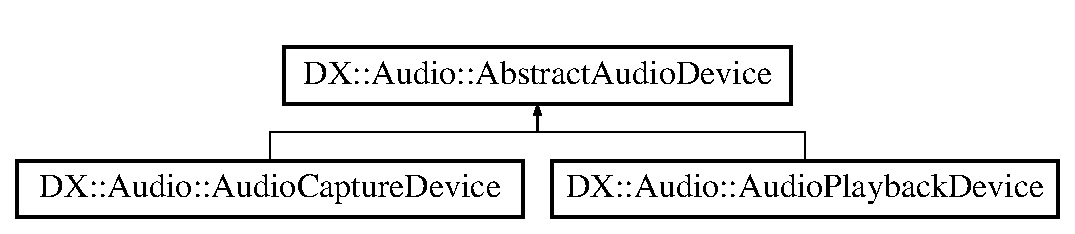
\includegraphics[height=2.000000cm]{class_d_x_1_1_audio_1_1_abstract_audio_device}
\end{center}
\end{figure}
\subsection*{Public Member Functions}
\begin{DoxyCompactItemize}
\item 
\hypertarget{class_d_x_1_1_audio_1_1_abstract_audio_device_a7992aa69af2eb4fbee273e84e08e244b}{virtual bool {\bfseries initialize} ()=0}\label{class_d_x_1_1_audio_1_1_abstract_audio_device_a7992aa69af2eb4fbee273e84e08e244b}

\item 
\hypertarget{class_d_x_1_1_audio_1_1_abstract_audio_device_acac63db656c17373196be255750bfb4d}{virtual bool {\bfseries start} ()}\label{class_d_x_1_1_audio_1_1_abstract_audio_device_acac63db656c17373196be255750bfb4d}

\item 
\hypertarget{class_d_x_1_1_audio_1_1_abstract_audio_device_a1eb78fe6b16b4421f49e18e061d2d2ec}{virtual bool {\bfseries stop} ()}\label{class_d_x_1_1_audio_1_1_abstract_audio_device_a1eb78fe6b16b4421f49e18e061d2d2ec}

\item 
\hypertarget{class_d_x_1_1_audio_1_1_abstract_audio_device_aeee4fee106b42544b847e0a2c33af432}{virtual bool {\bfseries is\-Capture\-Device} () const }\label{class_d_x_1_1_audio_1_1_abstract_audio_device_aeee4fee106b42544b847e0a2c33af432}

\item 
\hypertarget{class_d_x_1_1_audio_1_1_abstract_audio_device_a630ff4626c9fa3dbea779425450a9f04}{virtual bool {\bfseries is\-Playback\-Device} () const }\label{class_d_x_1_1_audio_1_1_abstract_audio_device_a630ff4626c9fa3dbea779425450a9f04}

\item 
\hypertarget{class_d_x_1_1_audio_1_1_abstract_audio_device_ab5743c6b0c5412663f3ada8f87df8f9b}{virtual bool {\bfseries is\-Valid} () const }\label{class_d_x_1_1_audio_1_1_abstract_audio_device_ab5743c6b0c5412663f3ada8f87df8f9b}

\item 
\hypertarget{class_d_x_1_1_audio_1_1_abstract_audio_device_aeae655ba2f6613ca9a40248133c54ab3}{virtual \hyperlink{struct_d_x_1_1_audio_1_1_audio_format}{Audio\-Format} {\bfseries get\-Audio\-Format} () const }\label{class_d_x_1_1_audio_1_1_abstract_audio_device_aeae655ba2f6613ca9a40248133c54ab3}

\item 
\hypertarget{class_d_x_1_1_audio_1_1_abstract_audio_device_a9eb19e3e87d1ab53979784ce2744cc18}{virtual \hyperlink{class_d_x_1_1_audio_1_1_audio_packet}{Audio\-Packet} {\bfseries read\-From\-Buffer} ()=0}\label{class_d_x_1_1_audio_1_1_abstract_audio_device_a9eb19e3e87d1ab53979784ce2744cc18}

\item 
\hypertarget{class_d_x_1_1_audio_1_1_abstract_audio_device_adde4b9a7286575f90258da492e0d8f9b}{virtual bool {\bfseries read\-From\-Buffer} (\hyperlink{class_d_x_1_1_lock_free_1_1_concurrent_stream}{Audio\-Stream} \&out, \hyperlink{class_d_x_1_1_audio_1_1_task_callback}{Task\-Callback} $\ast$callback)=0}\label{class_d_x_1_1_audio_1_1_abstract_audio_device_adde4b9a7286575f90258da492e0d8f9b}

\item 
\hypertarget{class_d_x_1_1_audio_1_1_abstract_audio_device_a08c33a0e97d3919024976b8e1ef19800}{virtual bool {\bfseries write\-To\-Buffer} (const \hyperlink{class_d_x_1_1_audio_1_1_audio_packet}{Audio\-Packet} \&in, const \hyperlink{struct_d_x_1_1_audio_1_1_abstract_filter}{Abstract\-Filter} \&filter)=0}\label{class_d_x_1_1_audio_1_1_abstract_audio_device_a08c33a0e97d3919024976b8e1ef19800}

\item 
\hypertarget{class_d_x_1_1_audio_1_1_abstract_audio_device_a0c79b32fdd2720a5bc759a6baa6edca3}{virtual bool {\bfseries write\-To\-Buffer} (\hyperlink{class_d_x_1_1_lock_free_1_1_concurrent_stream}{Audio\-Stream} \&in, const \hyperlink{struct_d_x_1_1_audio_1_1_abstract_filter}{Abstract\-Filter} \&filter, \hyperlink{class_d_x_1_1_audio_1_1_task_callback}{Task\-Callback} $\ast$callback=nullptr)=0}\label{class_d_x_1_1_audio_1_1_abstract_audio_device_a0c79b32fdd2720a5bc759a6baa6edca3}

\item 
\hypertarget{class_d_x_1_1_audio_1_1_abstract_audio_device_a300d1e3c5fcdf11dc99c82c41fdb03b9}{virtual std\-::string {\bfseries id} () const }\label{class_d_x_1_1_audio_1_1_abstract_audio_device_a300d1e3c5fcdf11dc99c82c41fdb03b9}

\end{DoxyCompactItemize}
\subsection*{Protected Member Functions}
\begin{DoxyCompactItemize}
\item 
\hypertarget{class_d_x_1_1_audio_1_1_abstract_audio_device_afe188c72c304c3ad1f7f77f779439c81}{{\bfseries Abstract\-Audio\-Device} (const \hyperlink{class_d_x_1_1_audio_1_1_abstract_audio_device}{Abstract\-Audio\-Device} \&)}\label{class_d_x_1_1_audio_1_1_abstract_audio_device_afe188c72c304c3ad1f7f77f779439c81}

\item 
\hypertarget{class_d_x_1_1_audio_1_1_abstract_audio_device_ab30ae887030ab1cf0facb2fa436d6e90}{{\bfseries Abstract\-Audio\-Device} (\hyperlink{class_d_x_1_1_audio_1_1_abstract_audio_device}{Abstract\-Audio\-Device} \&\&)}\label{class_d_x_1_1_audio_1_1_abstract_audio_device_ab30ae887030ab1cf0facb2fa436d6e90}

\end{DoxyCompactItemize}
\subsection*{Protected Attributes}
\begin{DoxyCompactItemize}
\item 
\hypertarget{class_d_x_1_1_audio_1_1_abstract_audio_device_a5cf5daa514cf4bb7baa2d7ddbd63af5a}{\hyperlink{classstd_1_1shared__ptr}{std\-::shared\-\_\-ptr}\\*
$<$ Abstract\-Audio\-Device\-Impl $>$ {\bfseries m\-\_\-impl}}\label{class_d_x_1_1_audio_1_1_abstract_audio_device_a5cf5daa514cf4bb7baa2d7ddbd63af5a}

\end{DoxyCompactItemize}
\subsection*{Friends}
\begin{DoxyCompactItemize}
\item 
\hypertarget{class_d_x_1_1_audio_1_1_abstract_audio_device_a04f96566766f09f439a3a13c5fcbe408}{class {\bfseries Audio\-Device\-Manager\-Impl}}\label{class_d_x_1_1_audio_1_1_abstract_audio_device_a04f96566766f09f439a3a13c5fcbe408}

\end{DoxyCompactItemize}


\subsection{Detailed Description}
\hyperlink{class_d_x_1_1_audio_1_1_abstract_audio_device}{Abstract\-Audio\-Device} is the base class for any system-\/recognized hardware. 

The documentation for this class was generated from the following files\-:\begin{DoxyCompactItemize}
\item 
Audio/Abstract\-Audio\-Device.\-h\item 
Audio/Abstract\-Audio\-Device.\-cpp\end{DoxyCompactItemize}

\hypertarget{class_d_x_1_1_audio_1_1_abstract_audio_task}{\section{D\-X\-:\-:Audio\-:\-:Abstract\-Audio\-Task Class Reference}
\label{class_d_x_1_1_audio_1_1_abstract_audio_task}\index{D\-X\-::\-Audio\-::\-Abstract\-Audio\-Task@{D\-X\-::\-Audio\-::\-Abstract\-Audio\-Task}}
}
\subsection*{Public Member Functions}
\begin{DoxyCompactItemize}
\item 
\hypertarget{class_d_x_1_1_audio_1_1_abstract_audio_task_abcfc1d6d6e9ce76cdb756f6b59e9980b}{{\bfseries Abstract\-Audio\-Task} (\hyperlink{class_d_x_1_1_audio_1_1_abstract_audio_device}{Abstract\-Audio\-Device} $\ast$device)}\label{class_d_x_1_1_audio_1_1_abstract_audio_task_abcfc1d6d6e9ce76cdb756f6b59e9980b}

\item 
\hypertarget{class_d_x_1_1_audio_1_1_abstract_audio_task_ac9e16dcb6c9b23e0703c1e3556b90a87}{virtual void {\bfseries run} (\hyperlink{class_d_x_1_1_audio_1_1_task_callback}{Task\-Callback} $\ast$callback=nullptr)=0}\label{class_d_x_1_1_audio_1_1_abstract_audio_task_ac9e16dcb6c9b23e0703c1e3556b90a87}

\end{DoxyCompactItemize}
\subsection*{Protected Attributes}
\begin{DoxyCompactItemize}
\item 
\hypertarget{class_d_x_1_1_audio_1_1_abstract_audio_task_a23ae17b2ecc403da3cfbd8d2c6ff527a}{\-::\hyperlink{classstd_1_1shared__ptr}{std\-::shared\-\_\-ptr}\\*
$<$ \hyperlink{class_d_x_1_1_audio_1_1_abstract_audio_device}{Abstract\-Audio\-Device} $>$ {\bfseries m\-\_\-device}}\label{class_d_x_1_1_audio_1_1_abstract_audio_task_a23ae17b2ecc403da3cfbd8d2c6ff527a}

\end{DoxyCompactItemize}


The documentation for this class was generated from the following file\-:\begin{DoxyCompactItemize}
\item 
Audio/\-Tasks/Abstract\-Audio\-Task.\-h\end{DoxyCompactItemize}

\hypertarget{class_d_x_1_1_lock_free_1_1_abstract_barrier}{\section{D\-X\-:\-:Lock\-Free\-:\-:Abstract\-Barrier Class Reference}
\label{class_d_x_1_1_lock_free_1_1_abstract_barrier}\index{D\-X\-::\-Lock\-Free\-::\-Abstract\-Barrier@{D\-X\-::\-Lock\-Free\-::\-Abstract\-Barrier}}
}


An \hyperlink{class_d_x_1_1_lock_free_1_1_abstract_barrier}{Abstract\-Barrier} is designed for use between multiple threads, typically blocking unparallelelizable sections of code. Any class derived off of an Abstract Barrier will block threads of execution at calls to \hyperlink{class_d_x_1_1_lock_free_1_1_abstract_barrier_a9040adf7507467e5a653bdaf2fbd17a6}{wait()} until \hyperlink{class_d_x_1_1_lock_free_1_1_abstract_barrier_a9040adf7507467e5a653bdaf2fbd17a6}{wait()} has been called some number of times, where that amount is defined by the number supplied to the constructor.  




{\ttfamily \#include $<$Abstract\-Barrier.\-h$>$}

Inheritance diagram for D\-X\-:\-:Lock\-Free\-:\-:Abstract\-Barrier\-:\begin{figure}[H]
\begin{center}
\leavevmode
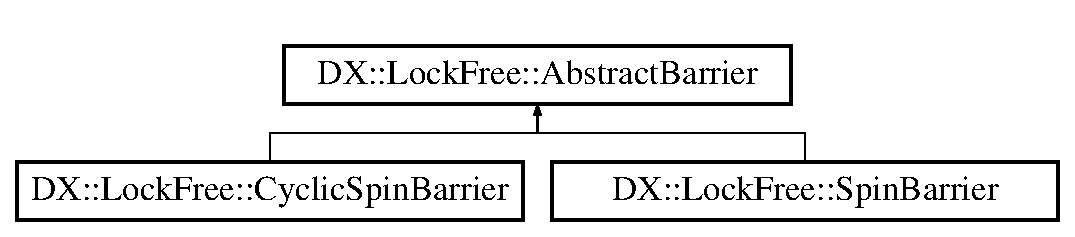
\includegraphics[height=2.000000cm]{class_d_x_1_1_lock_free_1_1_abstract_barrier}
\end{center}
\end{figure}
\subsection*{Public Member Functions}
\begin{DoxyCompactItemize}
\item 
\hyperlink{class_d_x_1_1_lock_free_1_1_abstract_barrier_a57ea820cef85c23cd631f56956ad667f}{Abstract\-Barrier} (size\-\_\-t num\-Threads)
\item 
virtual void \hyperlink{class_d_x_1_1_lock_free_1_1_abstract_barrier_a9040adf7507467e5a653bdaf2fbd17a6}{wait} () const =0
\end{DoxyCompactItemize}
\subsection*{Protected Attributes}
\begin{DoxyCompactItemize}
\item 
\hypertarget{class_d_x_1_1_lock_free_1_1_abstract_barrier_a17dd0c6e950114baf17495d62a00af5a}{volatile char {\bfseries pad\-\_\-0} \mbox{[}C\-A\-C\-H\-E\-\_\-\-L\-I\-N\-E\-\_\-\-S\-I\-Z\-E\mbox{]}}\label{class_d_x_1_1_lock_free_1_1_abstract_barrier_a17dd0c6e950114baf17495d62a00af5a}

\item 
\hypertarget{class_d_x_1_1_lock_free_1_1_abstract_barrier_a348b132862ba722bc278d07cd2d714c3}{std\-::atomic$<$ size\-\_\-t $>$ {\bfseries m\-\_\-count}}\label{class_d_x_1_1_lock_free_1_1_abstract_barrier_a348b132862ba722bc278d07cd2d714c3}

\item 
\hypertarget{class_d_x_1_1_lock_free_1_1_abstract_barrier_a3127ea3626fcce39c5534ec5e485fe13}{volatile char {\bfseries pad\-\_\-1} \mbox{[}C\-A\-C\-H\-E\-\_\-\-L\-I\-N\-E\-\_\-\-S\-I\-Z\-E-\/(sizeof(std\-::atomic$<$ size\-\_\-t $>$)\%C\-A\-C\-H\-E\-\_\-\-L\-I\-N\-E\-\_\-\-S\-I\-Z\-E)\mbox{]}}\label{class_d_x_1_1_lock_free_1_1_abstract_barrier_a3127ea3626fcce39c5534ec5e485fe13}

\end{DoxyCompactItemize}


\subsection{Detailed Description}
An \hyperlink{class_d_x_1_1_lock_free_1_1_abstract_barrier}{Abstract\-Barrier} is designed for use between multiple threads, typically blocking unparallelelizable sections of code. Any class derived off of an Abstract Barrier will block threads of execution at calls to \hyperlink{class_d_x_1_1_lock_free_1_1_abstract_barrier_a9040adf7507467e5a653bdaf2fbd17a6}{wait()} until \hyperlink{class_d_x_1_1_lock_free_1_1_abstract_barrier_a9040adf7507467e5a653bdaf2fbd17a6}{wait()} has been called some number of times, where that amount is defined by the number supplied to the constructor. 

Behavior is undefined if the number of threads to wait on is 0 or 1.

A contrived use case is for scatter and gather\-:


\begin{DoxyCode}
\textcolor{keywordtype}{void} processWork(\hyperlink{class_d_x_1_1_lock_free_1_1_abstract_barrier_a57ea820cef85c23cd631f56956ad667f}{AbstractBarrier}& barrier)
\{
    \textcolor{comment}{// Do some work}
    barrier.wait();
\}

\textcolor{keywordtype}{void} scatter()
\{
    \textcolor{comment}{// + 1 here, because we want to block the main thread of execution as well}
    \hyperlink{class_d_x_1_1_lock_free_1_1_abstract_barrier_a57ea820cef85c23cd631f56956ad667f}{AbstractBarrier} barrier(someNumberOfThreads );
    \textcolor{keywordflow}{for}(\textcolor{keywordtype}{int} i = 0; i < someNumberOfThreads; ++i)
        std::thread(&processWork, barrier);

    barrier.wait();
    gather();
\}

\textcolor{keywordtype}{void} gather()
\{
    \textcolor{comment}{// Do some other stuff }

    \textcolor{comment}{//Here, scatter() has ensured that gather will ONLY be called once all threads have}
    \textcolor{comment}{//completed their work.}
\}
\end{DoxyCode}
 

\subsection{Constructor \& Destructor Documentation}
\hypertarget{class_d_x_1_1_lock_free_1_1_abstract_barrier_a57ea820cef85c23cd631f56956ad667f}{\index{D\-X\-::\-Lock\-Free\-::\-Abstract\-Barrier@{D\-X\-::\-Lock\-Free\-::\-Abstract\-Barrier}!Abstract\-Barrier@{Abstract\-Barrier}}
\index{Abstract\-Barrier@{Abstract\-Barrier}!DX::LockFree::AbstractBarrier@{D\-X\-::\-Lock\-Free\-::\-Abstract\-Barrier}}
\subsubsection[{Abstract\-Barrier}]{\setlength{\rightskip}{0pt plus 5cm}D\-X\-::\-Lock\-Free\-::\-Abstract\-Barrier\-::\-Abstract\-Barrier (
\begin{DoxyParamCaption}
\item[{size\-\_\-t}]{num\-Threads}
\end{DoxyParamCaption}
)\hspace{0.3cm}{\ttfamily [explicit]}}}\label{class_d_x_1_1_lock_free_1_1_abstract_barrier_a57ea820cef85c23cd631f56956ad667f}
Constructs an \hyperlink{class_d_x_1_1_lock_free_1_1_abstract_barrier}{Abstract\-Barrier} that is set up to wait on some number of threads 
\begin{DoxyParams}[1]{Parameters}
\mbox{\tt in}  & {\em num\-Threads} & The number of threads that are expected to use this barrier \\
\hline
\end{DoxyParams}


\subsection{Member Function Documentation}
\hypertarget{class_d_x_1_1_lock_free_1_1_abstract_barrier_a9040adf7507467e5a653bdaf2fbd17a6}{\index{D\-X\-::\-Lock\-Free\-::\-Abstract\-Barrier@{D\-X\-::\-Lock\-Free\-::\-Abstract\-Barrier}!wait@{wait}}
\index{wait@{wait}!DX::LockFree::AbstractBarrier@{D\-X\-::\-Lock\-Free\-::\-Abstract\-Barrier}}
\subsubsection[{wait}]{\setlength{\rightskip}{0pt plus 5cm}virtual void D\-X\-::\-Lock\-Free\-::\-Abstract\-Barrier\-::wait (
\begin{DoxyParamCaption}
{}
\end{DoxyParamCaption}
) const\hspace{0.3cm}{\ttfamily [pure virtual]}}}\label{class_d_x_1_1_lock_free_1_1_abstract_barrier_a9040adf7507467e5a653bdaf2fbd17a6}
Blocks the current thread of execution until all other \hyperlink{class_d_x_1_1_lock_free_1_1_abstract_barrier_a9040adf7507467e5a653bdaf2fbd17a6}{wait()} calls have beem made 

Implemented in \hyperlink{class_d_x_1_1_lock_free_1_1_cyclic_spin_barrier_af9b42b0455c7251bda38694a2df17d11}{D\-X\-::\-Lock\-Free\-::\-Cyclic\-Spin\-Barrier}, and \hyperlink{class_d_x_1_1_lock_free_1_1_spin_barrier_a869688c05d8edae270a0e549c36c163d}{D\-X\-::\-Lock\-Free\-::\-Spin\-Barrier}.



The documentation for this class was generated from the following files\-:\begin{DoxyCompactItemize}
\item 
Lock\-Free/\-Mutex/Abstract\-Barrier.\-h\item 
Lock\-Free/\-Mutex/Abstract\-Barrier.\-cpp\end{DoxyCompactItemize}

\hypertarget{struct_d_x_1_1_audio_1_1_abstract_filter}{\section{D\-X\-:\-:Audio\-:\-:Abstract\-Filter Struct Reference}
\label{struct_d_x_1_1_audio_1_1_abstract_filter}\index{D\-X\-::\-Audio\-::\-Abstract\-Filter@{D\-X\-::\-Audio\-::\-Abstract\-Filter}}
}
Inheritance diagram for D\-X\-:\-:Audio\-:\-:Abstract\-Filter\-:\begin{figure}[H]
\begin{center}
\leavevmode
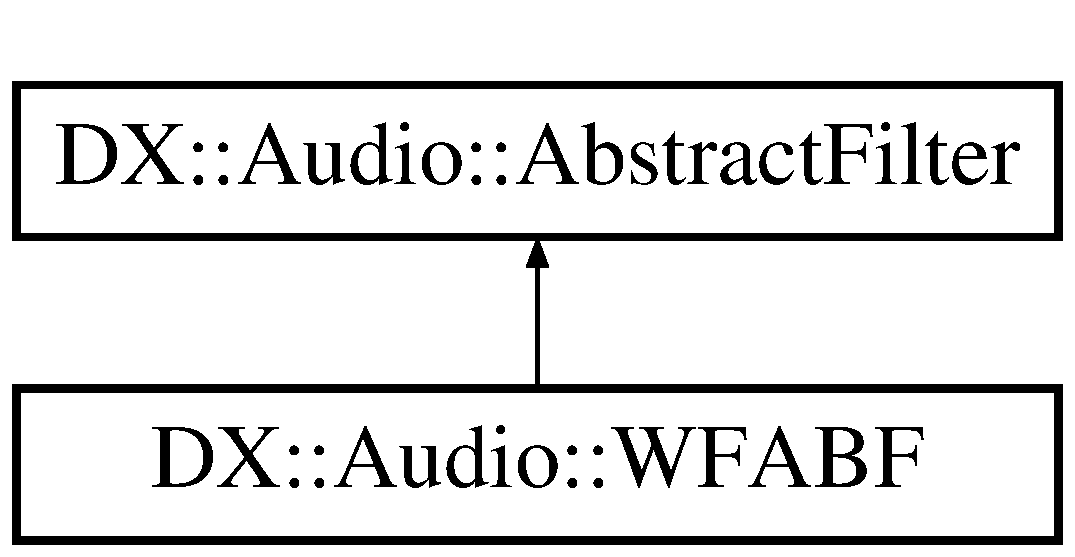
\includegraphics[height=2.000000cm]{struct_d_x_1_1_audio_1_1_abstract_filter}
\end{center}
\end{figure}
\subsection*{Public Member Functions}
\begin{DoxyCompactItemize}
\item 
\hypertarget{struct_d_x_1_1_audio_1_1_abstract_filter_aa8bb18f87a623d1c03bf309ec3797d89}{{\bfseries Abstract\-Filter} (\hyperlink{classstd_1_1shared__ptr}{std\-::shared\-\_\-ptr}$<$ \hyperlink{struct_d_x_1_1_audio_1_1_abstract_filter}{Abstract\-Filter} $>$ filter, Filter\-Type type)}\label{struct_d_x_1_1_audio_1_1_abstract_filter_aa8bb18f87a623d1c03bf309ec3797d89}

\item 
\hypertarget{struct_d_x_1_1_audio_1_1_abstract_filter_a699796aa423c93b29a8d7f862dfba5e8}{virtual bool {\bfseries transform\-Packet} (const \hyperlink{class_d_x_1_1_audio_1_1_audio_packet}{Audio\-Packet} \&in, \hyperlink{class_d_x_1_1_audio_1_1_audio_packet}{Audio\-Packet} \&out) const =0}\label{struct_d_x_1_1_audio_1_1_abstract_filter_a699796aa423c93b29a8d7f862dfba5e8}

\item 
\hypertarget{struct_d_x_1_1_audio_1_1_abstract_filter_a590c1f45b9d7b5334489b13e68c61495}{virtual std\-::string {\bfseries name} () const =0}\label{struct_d_x_1_1_audio_1_1_abstract_filter_a590c1f45b9d7b5334489b13e68c61495}

\end{DoxyCompactItemize}


The documentation for this struct was generated from the following files\-:\begin{DoxyCompactItemize}
\item 
Audio/\-Filters/Abstract\-Filter.\-h\item 
Audio/\-Filters/Abstract\-Filter.\-cpp\end{DoxyCompactItemize}

\hypertarget{class_d_x_1_1_audio_1_1_audio_capture_device}{\section{D\-X\-:\-:Audio\-:\-:Audio\-Capture\-Device Class Reference}
\label{class_d_x_1_1_audio_1_1_audio_capture_device}\index{D\-X\-::\-Audio\-::\-Audio\-Capture\-Device@{D\-X\-::\-Audio\-::\-Audio\-Capture\-Device}}
}
Inheritance diagram for D\-X\-:\-:Audio\-:\-:Audio\-Capture\-Device\-:\begin{figure}[H]
\begin{center}
\leavevmode
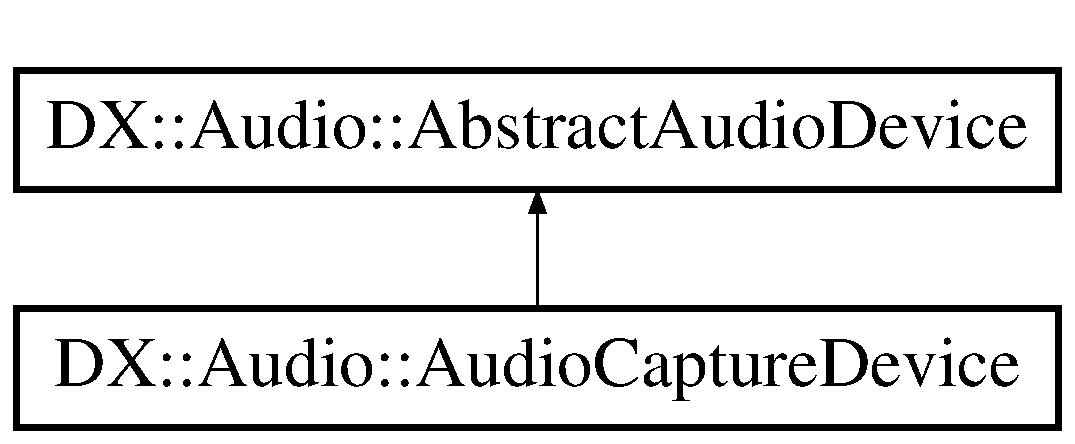
\includegraphics[height=2.000000cm]{class_d_x_1_1_audio_1_1_audio_capture_device}
\end{center}
\end{figure}
\subsection*{Public Member Functions}
\begin{DoxyCompactItemize}
\item 
\hypertarget{class_d_x_1_1_audio_1_1_audio_capture_device_a5ddf885c345d4ccf08b43dbc1c19784f}{virtual bool {\bfseries initialize} ()}\label{class_d_x_1_1_audio_1_1_audio_capture_device_a5ddf885c345d4ccf08b43dbc1c19784f}

\item 
\hypertarget{class_d_x_1_1_audio_1_1_audio_capture_device_acb57e48a6ca54178ee16ac27cfd7c483}{virtual bool {\bfseries is\-Capture\-Device} () const }\label{class_d_x_1_1_audio_1_1_audio_capture_device_acb57e48a6ca54178ee16ac27cfd7c483}

\item 
\hypertarget{class_d_x_1_1_audio_1_1_audio_capture_device_adf79121ec0570247120739a3d2df0af3}{virtual \hyperlink{class_d_x_1_1_audio_1_1_audio_packet}{Audio\-Packet} {\bfseries read\-From\-Buffer} ()}\label{class_d_x_1_1_audio_1_1_audio_capture_device_adf79121ec0570247120739a3d2df0af3}

\item 
\hypertarget{class_d_x_1_1_audio_1_1_audio_capture_device_a188bf18aae62acbdc9d205753529317c}{virtual bool {\bfseries read\-From\-Buffer} (\hyperlink{class_d_x_1_1_lock_free_1_1_concurrent_stream}{Audio\-Stream} \&out, \hyperlink{class_d_x_1_1_audio_1_1_task_callback}{Task\-Callback} $\ast$callback)}\label{class_d_x_1_1_audio_1_1_audio_capture_device_a188bf18aae62acbdc9d205753529317c}

\item 
\hypertarget{class_d_x_1_1_audio_1_1_audio_capture_device_ae3ef3d8ab13553e0a7e081960591273c}{virtual bool {\bfseries write\-To\-Buffer} (const \hyperlink{class_d_x_1_1_audio_1_1_audio_packet}{Audio\-Packet} \&in, const \hyperlink{struct_d_x_1_1_audio_1_1_abstract_filter}{Abstract\-Filter} \&filter)}\label{class_d_x_1_1_audio_1_1_audio_capture_device_ae3ef3d8ab13553e0a7e081960591273c}

\item 
\hypertarget{class_d_x_1_1_audio_1_1_audio_capture_device_af0a0c34af91c30d60dedf754c5ecd916}{virtual bool {\bfseries write\-To\-Buffer} (\hyperlink{class_d_x_1_1_lock_free_1_1_concurrent_stream}{Audio\-Stream} \&in, const \hyperlink{struct_d_x_1_1_audio_1_1_abstract_filter}{Abstract\-Filter} \&filter, \hyperlink{class_d_x_1_1_audio_1_1_task_callback}{Task\-Callback} $\ast$callback)}\label{class_d_x_1_1_audio_1_1_audio_capture_device_af0a0c34af91c30d60dedf754c5ecd916}

\end{DoxyCompactItemize}
\subsection*{Additional Inherited Members}


The documentation for this class was generated from the following files\-:\begin{DoxyCompactItemize}
\item 
Audio/Audio\-Capture\-Device.\-h\item 
Audio/Audio\-Capture\-Device.\-cpp\end{DoxyCompactItemize}

\hypertarget{class_d_x_1_1_audio_1_1_audio_device_manager}{\section{D\-X\-:\-:Audio\-:\-:Audio\-Device\-Manager Class Reference}
\label{class_d_x_1_1_audio_1_1_audio_device_manager}\index{D\-X\-::\-Audio\-::\-Audio\-Device\-Manager@{D\-X\-::\-Audio\-::\-Audio\-Device\-Manager}}
}
\subsection*{Public Member Functions}
\begin{DoxyCompactItemize}
\item 
\hypertarget{class_d_x_1_1_audio_1_1_audio_device_manager_aa9dba80633884865cc49c70483a32b21}{bool {\bfseries initialize} ()}\label{class_d_x_1_1_audio_1_1_audio_device_manager_aa9dba80633884865cc49c70483a32b21}

\item 
\hypertarget{class_d_x_1_1_audio_1_1_audio_device_manager_a1a08f67dd007894212e5e1aaff0c18bf}{bool {\bfseries un\-Initialize} ()}\label{class_d_x_1_1_audio_1_1_audio_device_manager_a1a08f67dd007894212e5e1aaff0c18bf}

\item 
\hypertarget{class_d_x_1_1_audio_1_1_audio_device_manager_a4b977076115ff0408bd09c73d8852287}{std\-::vector$<$ \hyperlink{classstd_1_1shared__ptr}{std\-::shared\-\_\-ptr}\\*
$<$ \hyperlink{class_d_x_1_1_audio_1_1_audio_playback_device}{Audio\-Playback\-Device} $>$ $>$ {\bfseries get\-Playback\-Devices} () const }\label{class_d_x_1_1_audio_1_1_audio_device_manager_a4b977076115ff0408bd09c73d8852287}

\item 
\hypertarget{class_d_x_1_1_audio_1_1_audio_device_manager_a353d7ceb8444ea742313cf290aff5820}{std\-::vector$<$ \hyperlink{classstd_1_1shared__ptr}{std\-::shared\-\_\-ptr}\\*
$<$ \hyperlink{class_d_x_1_1_audio_1_1_audio_capture_device}{Audio\-Capture\-Device} $>$ $>$ {\bfseries get\-Capture\-Devices} () const }\label{class_d_x_1_1_audio_1_1_audio_device_manager_a353d7ceb8444ea742313cf290aff5820}

\item 
\hypertarget{class_d_x_1_1_audio_1_1_audio_device_manager_afe6a0b08ac3b2673eb3645a03a1de00d}{std\-::vector$<$ \hyperlink{classstd_1_1shared__ptr}{std\-::shared\-\_\-ptr}\\*
$<$ \hyperlink{class_d_x_1_1_audio_1_1_abstract_audio_device}{Abstract\-Audio\-Device} $>$ $>$ {\bfseries get\-All\-Devices} () const }\label{class_d_x_1_1_audio_1_1_audio_device_manager_afe6a0b08ac3b2673eb3645a03a1de00d}

\item 
\hypertarget{class_d_x_1_1_audio_1_1_audio_device_manager_a49c4f030d2ba717e276f280175106bea}{\hyperlink{classstd_1_1shared__ptr}{std\-::shared\-\_\-ptr}\\*
$<$ \hyperlink{class_d_x_1_1_audio_1_1_audio_capture_device}{Audio\-Capture\-Device} $>$ {\bfseries get\-Default\-Capture\-Device} () const }\label{class_d_x_1_1_audio_1_1_audio_device_manager_a49c4f030d2ba717e276f280175106bea}

\item 
\hypertarget{class_d_x_1_1_audio_1_1_audio_device_manager_af0c7d3753866aaabda01b1927ba5bff1}{\hyperlink{classstd_1_1shared__ptr}{std\-::shared\-\_\-ptr}\\*
$<$ \hyperlink{class_d_x_1_1_audio_1_1_audio_playback_device}{Audio\-Playback\-Device} $>$ {\bfseries get\-Default\-Playback\-Device} () const }\label{class_d_x_1_1_audio_1_1_audio_device_manager_af0c7d3753866aaabda01b1927ba5bff1}

\item 
\hypertarget{class_d_x_1_1_audio_1_1_audio_device_manager_a6c837df31f4e2c203fc835c358e19bd9}{\hyperlink{classstd_1_1shared__ptr}{std\-::shared\-\_\-ptr}\\*
$<$ \hyperlink{class_d_x_1_1_audio_1_1_audio_capture_device}{Audio\-Capture\-Device} $>$ {\bfseries get\-Default\-Playback\-Device\-As\-Capture\-Device} () const }\label{class_d_x_1_1_audio_1_1_audio_device_manager_a6c837df31f4e2c203fc835c358e19bd9}

\item 
\hypertarget{class_d_x_1_1_audio_1_1_audio_device_manager_a533f5df8679fd4dee7d890d27aaa0fd0}{bool {\bfseries is\-Initialized} () const }\label{class_d_x_1_1_audio_1_1_audio_device_manager_a533f5df8679fd4dee7d890d27aaa0fd0}

\end{DoxyCompactItemize}


The documentation for this class was generated from the following files\-:\begin{DoxyCompactItemize}
\item 
Audio/Audio\-Device\-Manager.\-h\item 
Audio/Audio\-Device\-Manager.\-cpp\end{DoxyCompactItemize}

\hypertarget{struct_d_x_1_1_audio_1_1_audio_format}{\section{D\-X\-:\-:Audio\-:\-:Audio\-Format Struct Reference}
\label{struct_d_x_1_1_audio_1_1_audio_format}\index{D\-X\-::\-Audio\-::\-Audio\-Format@{D\-X\-::\-Audio\-::\-Audio\-Format}}
}


\hyperlink{struct_d_x_1_1_audio_1_1_audio_format}{Audio\-Format} is a lightweight tag structure designed to attach to things that need some kind of audio format information. This typically includes hardware audio devices, where the information is pulled from, Streams to and from devices, and Audio\-Packets themselves. Streams and Audio\-Packets especially can be passed around freely. Any given class accessing them may want to know the format or any additional information about the data contained, as otherwise, the data would be contextless and largely useless.  




{\ttfamily \#include $<$Audio\-Format.\-h$>$}

\subsection*{Public Member Functions}
\begin{DoxyCompactItemize}
\item 
\hypertarget{struct_d_x_1_1_audio_1_1_audio_format_aba69717f1269cb30d2f81aea5d17dfc5}{bool {\bfseries operator==} (const \hyperlink{struct_d_x_1_1_audio_1_1_audio_format}{Audio\-Format} \&other) const }\label{struct_d_x_1_1_audio_1_1_audio_format_aba69717f1269cb30d2f81aea5d17dfc5}

\item 
\hypertarget{struct_d_x_1_1_audio_1_1_audio_format_a93e1ebaa455c04c246413c3217f12e91}{bool {\bfseries operator!=} (const \hyperlink{struct_d_x_1_1_audio_1_1_audio_format}{Audio\-Format} \&other) const }\label{struct_d_x_1_1_audio_1_1_audio_format_a93e1ebaa455c04c246413c3217f12e91}

\end{DoxyCompactItemize}
\subsection*{Public Attributes}
\begin{DoxyCompactItemize}
\item 
unsigned short \hyperlink{struct_d_x_1_1_audio_1_1_audio_format_a99e6f97c11da52c68bb1cedc98dfe341}{channels}
\item 
unsigned int \hyperlink{struct_d_x_1_1_audio_1_1_audio_format_ae38016a3233f056484d95808eb53f781}{samples\-Per\-Second}
\item 
unsigned short \hyperlink{struct_d_x_1_1_audio_1_1_audio_format_aa6e6a2856d9afcd3b450f25316557c7b}{bits\-Per\-Block}
\item 
unsigned int \hyperlink{struct_d_x_1_1_audio_1_1_audio_format_a2e624e38652b39d310149e7a2259a4ee}{bits\-Per\-Sample}
\end{DoxyCompactItemize}


\subsection{Detailed Description}
\hyperlink{struct_d_x_1_1_audio_1_1_audio_format}{Audio\-Format} is a lightweight tag structure designed to attach to things that need some kind of audio format information. This typically includes hardware audio devices, where the information is pulled from, Streams to and from devices, and Audio\-Packets themselves. Streams and Audio\-Packets especially can be passed around freely. Any given class accessing them may want to know the format or any additional information about the data contained, as otherwise, the data would be contextless and largely useless. 

\begin{DoxyNote}{Note}
This will be expanded upon to contain any further useful information as the need arises. (Specifically, regarding support for platforms other than W\-I\-N32)
\end{DoxyNote}
This class should be able to accurately describe all common audio formats as well as any potential custom formats that may or may not exist. Filters should have the capability to adapt to any possible sampling frequency, channel count, bit depth, and sample size. A \char`\"{}typical\char`\"{} \hyperlink{struct_d_x_1_1_audio_1_1_audio_format}{Audio\-Format} will feature something like\-: channels = 2 samples\-Per\-Second = 44100 bits\-Per\-Block = 8 bits\-Per\-Sample = 32

For a 44.\-1 K\-Hz, 16-\/bit depth audio format 

\subsection{Member Data Documentation}
\hypertarget{struct_d_x_1_1_audio_1_1_audio_format_aa6e6a2856d9afcd3b450f25316557c7b}{\index{D\-X\-::\-Audio\-::\-Audio\-Format@{D\-X\-::\-Audio\-::\-Audio\-Format}!bits\-Per\-Block@{bits\-Per\-Block}}
\index{bits\-Per\-Block@{bits\-Per\-Block}!DX::Audio::AudioFormat@{D\-X\-::\-Audio\-::\-Audio\-Format}}
\subsubsection[{bits\-Per\-Block}]{\setlength{\rightskip}{0pt plus 5cm}unsigned short D\-X\-::\-Audio\-::\-Audio\-Format\-::bits\-Per\-Block}}\label{struct_d_x_1_1_audio_1_1_audio_format_aa6e6a2856d9afcd3b450f25316557c7b}
Number of bits to align a single block to \hypertarget{struct_d_x_1_1_audio_1_1_audio_format_a2e624e38652b39d310149e7a2259a4ee}{\index{D\-X\-::\-Audio\-::\-Audio\-Format@{D\-X\-::\-Audio\-::\-Audio\-Format}!bits\-Per\-Sample@{bits\-Per\-Sample}}
\index{bits\-Per\-Sample@{bits\-Per\-Sample}!DX::Audio::AudioFormat@{D\-X\-::\-Audio\-::\-Audio\-Format}}
\subsubsection[{bits\-Per\-Sample}]{\setlength{\rightskip}{0pt plus 5cm}unsigned int D\-X\-::\-Audio\-::\-Audio\-Format\-::bits\-Per\-Sample}}\label{struct_d_x_1_1_audio_1_1_audio_format_a2e624e38652b39d310149e7a2259a4ee}
Number of bits per sample of mono data \hypertarget{struct_d_x_1_1_audio_1_1_audio_format_a99e6f97c11da52c68bb1cedc98dfe341}{\index{D\-X\-::\-Audio\-::\-Audio\-Format@{D\-X\-::\-Audio\-::\-Audio\-Format}!channels@{channels}}
\index{channels@{channels}!DX::Audio::AudioFormat@{D\-X\-::\-Audio\-::\-Audio\-Format}}
\subsubsection[{channels}]{\setlength{\rightskip}{0pt plus 5cm}unsigned short D\-X\-::\-Audio\-::\-Audio\-Format\-::channels}}\label{struct_d_x_1_1_audio_1_1_audio_format_a99e6f97c11da52c68bb1cedc98dfe341}
Number of channels that the \hyperlink{struct_d_x_1_1_audio_1_1_audio_format}{Audio\-Format} has data for \hypertarget{struct_d_x_1_1_audio_1_1_audio_format_ae38016a3233f056484d95808eb53f781}{\index{D\-X\-::\-Audio\-::\-Audio\-Format@{D\-X\-::\-Audio\-::\-Audio\-Format}!samples\-Per\-Second@{samples\-Per\-Second}}
\index{samples\-Per\-Second@{samples\-Per\-Second}!DX::Audio::AudioFormat@{D\-X\-::\-Audio\-::\-Audio\-Format}}
\subsubsection[{samples\-Per\-Second}]{\setlength{\rightskip}{0pt plus 5cm}unsigned int D\-X\-::\-Audio\-::\-Audio\-Format\-::samples\-Per\-Second}}\label{struct_d_x_1_1_audio_1_1_audio_format_ae38016a3233f056484d95808eb53f781}
Frequency of sound that the \hyperlink{struct_d_x_1_1_audio_1_1_audio_format}{Audio\-Format} represents 

The documentation for this struct was generated from the following files\-:\begin{DoxyCompactItemize}
\item 
Audio/Audio\-Format.\-h\item 
Audio/Audio\-Format.\-cpp\end{DoxyCompactItemize}

\hypertarget{class_d_x_1_1_audio_1_1_audio_packet}{\section{D\-X\-:\-:Audio\-:\-:Audio\-Packet Class Reference}
\label{class_d_x_1_1_audio_1_1_audio_packet}\index{D\-X\-::\-Audio\-::\-Audio\-Packet@{D\-X\-::\-Audio\-::\-Audio\-Packet}}
}


\hyperlink{class_d_x_1_1_audio_1_1_audio_packet}{Audio\-Packet} is designed to hold a chunk of Audio\-Samples for hardware waveform I\-O. The simplest way of thinking about the class is as an array of \hyperlink{class_d_x_1_1_audio_1_1_audio_sample}{Audio\-Sample}. Audio\-Packets manage their own memory and have many useful functions, such as raw data access as well as array-\/like access.  




{\ttfamily \#include $<$Audio\-Packet.\-h$>$}

\subsection*{Public Member Functions}
\begin{DoxyCompactItemize}
\item 
\hyperlink{class_d_x_1_1_audio_1_1_audio_packet_a1086b8c3a23adbddf3dfa5706f0f7b04}{Audio\-Packet} (size\-\_\-t size=D\-E\-F\-A\-U\-L\-T\-\_\-\-P\-A\-C\-K\-E\-T\-\_\-\-S\-I\-Z\-E)
\begin{DoxyCompactList}\small\item\em Constructs an \hyperlink{class_d_x_1_1_audio_1_1_audio_packet}{Audio\-Packet} with D\-E\-F\-A\-U\-L\-T\-\_\-\-P\-A\-C\-K\-E\-T\-\_\-\-S\-I\-Z\-E number of Audio\-Bytes. \end{DoxyCompactList}\item 
\hyperlink{class_d_x_1_1_audio_1_1_audio_packet_a14c8e9755e1ac8bb386c1a8a62dd6058}{Audio\-Packet} (const \hyperlink{struct_d_x_1_1_audio_1_1_audio_format}{Audio\-Format} \&format, size\-\_\-t size=D\-E\-F\-A\-U\-L\-T\-\_\-\-P\-A\-C\-K\-E\-T\-\_\-\-S\-I\-Z\-E)
\begin{DoxyCompactList}\small\item\em Constructs an \hyperlink{class_d_x_1_1_audio_1_1_audio_packet}{Audio\-Packet} based off of a given \hyperlink{struct_d_x_1_1_audio_1_1_audio_format}{Audio\-Format} and a size representing the number of bytes that the \hyperlink{class_d_x_1_1_audio_1_1_audio_packet}{Audio\-Packet} should hold. \end{DoxyCompactList}\item 
\hyperlink{class_d_x_1_1_audio_1_1_audio_packet_a31534a4d2d2e8e10f95bf256055418f6}{Audio\-Packet} (const \hyperlink{class_d_x_1_1_audio_1_1_audio_packet}{Audio\-Packet} \&copy)
\item 
\hyperlink{class_d_x_1_1_audio_1_1_audio_packet_ac0554258f103fc1f9a21fdf90d6405fb}{Audio\-Packet} (\hyperlink{class_d_x_1_1_audio_1_1_audio_packet}{Audio\-Packet} \&\&move)
\item 
\hyperlink{class_d_x_1_1_audio_1_1_audio_packet_a0ef397ec1f3cbc296a5e06ffe9051f60}{$\sim$\-Audio\-Packet} ()
\item 
\hyperlink{class_d_x_1_1_audio_1_1_audio_sample}{Audio\-Sample} \hyperlink{class_d_x_1_1_audio_1_1_audio_packet_aaedb59240e8d6b8f77266fcd23ed9ab1}{operator\mbox{[}$\,$\mbox{]}} (size\-\_\-t index)
\item 
const \hyperlink{class_d_x_1_1_audio_1_1_audio_sample}{Audio\-Sample} \hyperlink{class_d_x_1_1_audio_1_1_audio_packet_a279dcbea3ad12838ceb819ab9639362e}{at} (size\-\_\-t index) const 
\item 
\hyperlink{class_d_x_1_1_audio_1_1_audio_packet}{Audio\-Packet} \& \hyperlink{class_d_x_1_1_audio_1_1_audio_packet_a8fe0f4f40e27254a64999186199533b6}{operator=} (\hyperlink{class_d_x_1_1_audio_1_1_audio_packet}{Audio\-Packet} \&\&move)
\item 
\hyperlink{class_d_x_1_1_audio_1_1_audio_packet}{Audio\-Packet} \& \hyperlink{class_d_x_1_1_audio_1_1_audio_packet_a9a18c4601eff6961aeeccfa799a11575}{operator=} (const \hyperlink{class_d_x_1_1_audio_1_1_audio_packet}{Audio\-Packet} \&copy)
\item 
\hyperlink{struct_d_x_1_1_audio_1_1_audio_format}{Audio\-Format} \hyperlink{class_d_x_1_1_audio_1_1_audio_packet_a6f47aa2be747ce054c5c68d723fbf64b}{get\-Audio\-Format} () const 
\item 
void \hyperlink{class_d_x_1_1_audio_1_1_audio_packet_a6d3120521532e6cd050b517ebed8f263}{set\-Audio\-Format} (const \hyperlink{struct_d_x_1_1_audio_1_1_audio_format}{Audio\-Format} \&)
\item 
size\-\_\-t \hyperlink{class_d_x_1_1_audio_1_1_audio_packet_a21f03d6b228c4ef5f3a85109b5e537a5}{byte\-Size} () const 
\item 
size\-\_\-t \hyperlink{class_d_x_1_1_audio_1_1_audio_packet_aa3e1275d86a76f1d42d4d5a4b6213e5f}{max\-Size} () const 
\item 
size\-\_\-t \hyperlink{class_d_x_1_1_audio_1_1_audio_packet_a2f98b04776946df7c3ccb4a0e5b80ce4}{num\-Samples} () const 
\item 
bool \hyperlink{class_d_x_1_1_audio_1_1_audio_packet_a75854e87ae3c4ce04503a75d42219ca5}{is\-Valid} () const 
\item 
Audio\-Byte $\ast$ \hyperlink{class_d_x_1_1_audio_1_1_audio_packet_ab93eafc041e06976f99fad9d21cc19e3}{data} ()
\begin{DoxyCompactList}\small\item\em Returns a pointer to the raw data held by the \hyperlink{class_d_x_1_1_audio_1_1_audio_packet}{Audio\-Packet}. \end{DoxyCompactList}\item 
const Audio\-Byte $\ast$ \hyperlink{class_d_x_1_1_audio_1_1_audio_packet_a24b0feecae93675256e4edb05cebe3fe}{data} () const 
\begin{DoxyCompactList}\small\item\em Returns a read-\/only pointer to the raw data held by the \hyperlink{class_d_x_1_1_audio_1_1_audio_packet}{Audio\-Packet}. \end{DoxyCompactList}\item 
void \hyperlink{class_d_x_1_1_audio_1_1_audio_packet_ad9686c0ca56c4da211514a8eadea8e5f}{assign} (const void $\ast$\hyperlink{class_d_x_1_1_audio_1_1_audio_packet_ab93eafc041e06976f99fad9d21cc19e3}{data}, size\-\_\-t num\-Bytes, size\-\_\-t offset=0)
\begin{DoxyCompactList}\small\item\em Assigns a chunk of memory to some location specified by off\-Set in the \hyperlink{class_d_x_1_1_audio_1_1_audio_packet}{Audio\-Packet}. \end{DoxyCompactList}\item 
void \hyperlink{class_d_x_1_1_audio_1_1_audio_packet_a0eef764bb6bf13de390740b1e35f04da}{assign} (std\-::unique\-\_\-ptr$<$ Audio\-Byte\mbox{[}$\,$\mbox{]}$>$ \&\&\hyperlink{class_d_x_1_1_audio_1_1_audio_packet_ab93eafc041e06976f99fad9d21cc19e3}{data})
\begin{DoxyCompactList}\small\item\em Moves a unique\-\_\-pointer representing some valid memory containing Audio\-Bytes. \end{DoxyCompactList}\end{DoxyCompactItemize}


\subsection{Detailed Description}
\hyperlink{class_d_x_1_1_audio_1_1_audio_packet}{Audio\-Packet} is designed to hold a chunk of Audio\-Samples for hardware waveform I\-O. The simplest way of thinking about the class is as an array of \hyperlink{class_d_x_1_1_audio_1_1_audio_sample}{Audio\-Sample}. Audio\-Packets manage their own memory and have many useful functions, such as raw data access as well as array-\/like access. 

\begin{DoxyNote}{Note}
operator\mbox{[}\mbox{]} and \hyperlink{class_d_x_1_1_audio_1_1_audio_packet_a279dcbea3ad12838ceb819ab9639362e}{at()} both return Audio\-Samples as opposed to pure Audio\-Bytes. This is for ease of Audio\-Filter / D\-S\-P creation 
\end{DoxyNote}


\subsection{Constructor \& Destructor Documentation}
\hypertarget{class_d_x_1_1_audio_1_1_audio_packet_a1086b8c3a23adbddf3dfa5706f0f7b04}{\index{D\-X\-::\-Audio\-::\-Audio\-Packet@{D\-X\-::\-Audio\-::\-Audio\-Packet}!Audio\-Packet@{Audio\-Packet}}
\index{Audio\-Packet@{Audio\-Packet}!DX::Audio::AudioPacket@{D\-X\-::\-Audio\-::\-Audio\-Packet}}
\subsubsection[{Audio\-Packet}]{\setlength{\rightskip}{0pt plus 5cm}D\-X\-::\-Audio\-::\-Audio\-Packet\-::\-Audio\-Packet (
\begin{DoxyParamCaption}
\item[{size\-\_\-t}]{size = {\ttfamily DEFAULT\-\_\-PACKET\-\_\-SIZE}}
\end{DoxyParamCaption}
)}}\label{class_d_x_1_1_audio_1_1_audio_packet_a1086b8c3a23adbddf3dfa5706f0f7b04}


Constructs an \hyperlink{class_d_x_1_1_audio_1_1_audio_packet}{Audio\-Packet} with D\-E\-F\-A\-U\-L\-T\-\_\-\-P\-A\-C\-K\-E\-T\-\_\-\-S\-I\-Z\-E number of Audio\-Bytes. 

\begin{DoxyNote}{Note}
The initial \hyperlink{struct_d_x_1_1_audio_1_1_audio_format}{Audio\-Format} for an \hyperlink{class_d_x_1_1_audio_1_1_audio_packet}{Audio\-Packet} constructed this way will be invalid 

No memory will be allocated if a size of 0 is provided 
\end{DoxyNote}
\hypertarget{class_d_x_1_1_audio_1_1_audio_packet_a14c8e9755e1ac8bb386c1a8a62dd6058}{\index{D\-X\-::\-Audio\-::\-Audio\-Packet@{D\-X\-::\-Audio\-::\-Audio\-Packet}!Audio\-Packet@{Audio\-Packet}}
\index{Audio\-Packet@{Audio\-Packet}!DX::Audio::AudioPacket@{D\-X\-::\-Audio\-::\-Audio\-Packet}}
\subsubsection[{Audio\-Packet}]{\setlength{\rightskip}{0pt plus 5cm}D\-X\-::\-Audio\-::\-Audio\-Packet\-::\-Audio\-Packet (
\begin{DoxyParamCaption}
\item[{const {\bf Audio\-Format} \&}]{format, }
\item[{size\-\_\-t}]{size = {\ttfamily DEFAULT\-\_\-PACKET\-\_\-SIZE}}
\end{DoxyParamCaption}
)}}\label{class_d_x_1_1_audio_1_1_audio_packet_a14c8e9755e1ac8bb386c1a8a62dd6058}


Constructs an \hyperlink{class_d_x_1_1_audio_1_1_audio_packet}{Audio\-Packet} based off of a given \hyperlink{struct_d_x_1_1_audio_1_1_audio_format}{Audio\-Format} and a size representing the number of bytes that the \hyperlink{class_d_x_1_1_audio_1_1_audio_packet}{Audio\-Packet} should hold. 

This is the preferred method of creating an \hyperlink{class_d_x_1_1_audio_1_1_audio_packet}{Audio\-Packet}. When typically creating an \hyperlink{class_d_x_1_1_audio_1_1_audio_packet}{Audio\-Packet}, both the \hyperlink{struct_d_x_1_1_audio_1_1_audio_format}{Audio\-Format} and byte amount should be readily available.

\begin{DoxyNote}{Note}
The size represents the number of Audio\-Bytes, not Audio\-Samples 
\end{DoxyNote}
\hypertarget{class_d_x_1_1_audio_1_1_audio_packet_a31534a4d2d2e8e10f95bf256055418f6}{\index{D\-X\-::\-Audio\-::\-Audio\-Packet@{D\-X\-::\-Audio\-::\-Audio\-Packet}!Audio\-Packet@{Audio\-Packet}}
\index{Audio\-Packet@{Audio\-Packet}!DX::Audio::AudioPacket@{D\-X\-::\-Audio\-::\-Audio\-Packet}}
\subsubsection[{Audio\-Packet}]{\setlength{\rightskip}{0pt plus 5cm}D\-X\-::\-Audio\-::\-Audio\-Packet\-::\-Audio\-Packet (
\begin{DoxyParamCaption}
\item[{const {\bf Audio\-Packet} \&}]{copy}
\end{DoxyParamCaption}
)}}\label{class_d_x_1_1_audio_1_1_audio_packet_a31534a4d2d2e8e10f95bf256055418f6}
Performs a deep copy on another \hyperlink{class_d_x_1_1_audio_1_1_audio_packet}{Audio\-Packet} \hypertarget{class_d_x_1_1_audio_1_1_audio_packet_ac0554258f103fc1f9a21fdf90d6405fb}{\index{D\-X\-::\-Audio\-::\-Audio\-Packet@{D\-X\-::\-Audio\-::\-Audio\-Packet}!Audio\-Packet@{Audio\-Packet}}
\index{Audio\-Packet@{Audio\-Packet}!DX::Audio::AudioPacket@{D\-X\-::\-Audio\-::\-Audio\-Packet}}
\subsubsection[{Audio\-Packet}]{\setlength{\rightskip}{0pt plus 5cm}D\-X\-::\-Audio\-::\-Audio\-Packet\-::\-Audio\-Packet (
\begin{DoxyParamCaption}
\item[{{\bf Audio\-Packet} \&\&}]{move}
\end{DoxyParamCaption}
)}}\label{class_d_x_1_1_audio_1_1_audio_packet_ac0554258f103fc1f9a21fdf90d6405fb}
Transfers ownership of \hyperlink{class_d_x_1_1_audio_1_1_audio_packet}{Audio\-Packet} resources \hypertarget{class_d_x_1_1_audio_1_1_audio_packet_a0ef397ec1f3cbc296a5e06ffe9051f60}{\index{D\-X\-::\-Audio\-::\-Audio\-Packet@{D\-X\-::\-Audio\-::\-Audio\-Packet}!$\sim$\-Audio\-Packet@{$\sim$\-Audio\-Packet}}
\index{$\sim$\-Audio\-Packet@{$\sim$\-Audio\-Packet}!DX::Audio::AudioPacket@{D\-X\-::\-Audio\-::\-Audio\-Packet}}
\subsubsection[{$\sim$\-Audio\-Packet}]{\setlength{\rightskip}{0pt plus 5cm}D\-X\-::\-Audio\-::\-Audio\-Packet\-::$\sim$\-Audio\-Packet (
\begin{DoxyParamCaption}
{}
\end{DoxyParamCaption}
)}}\label{class_d_x_1_1_audio_1_1_audio_packet_a0ef397ec1f3cbc296a5e06ffe9051f60}
Fully destroys all resources held by the \hyperlink{class_d_x_1_1_audio_1_1_audio_packet}{Audio\-Packet} 

\subsection{Member Function Documentation}
\hypertarget{class_d_x_1_1_audio_1_1_audio_packet_ad9686c0ca56c4da211514a8eadea8e5f}{\index{D\-X\-::\-Audio\-::\-Audio\-Packet@{D\-X\-::\-Audio\-::\-Audio\-Packet}!assign@{assign}}
\index{assign@{assign}!DX::Audio::AudioPacket@{D\-X\-::\-Audio\-::\-Audio\-Packet}}
\subsubsection[{assign}]{\setlength{\rightskip}{0pt plus 5cm}void D\-X\-::\-Audio\-::\-Audio\-Packet\-::assign (
\begin{DoxyParamCaption}
\item[{const void $\ast$}]{data, }
\item[{size\-\_\-t}]{num\-Bytes, }
\item[{size\-\_\-t}]{offset = {\ttfamily 0}}
\end{DoxyParamCaption}
)}}\label{class_d_x_1_1_audio_1_1_audio_packet_ad9686c0ca56c4da211514a8eadea8e5f}


Assigns a chunk of memory to some location specified by off\-Set in the \hyperlink{class_d_x_1_1_audio_1_1_audio_packet}{Audio\-Packet}. 


\begin{DoxyParams}[1]{Parameters}
\mbox{\tt in}  & {\em data} & A pointer to the data to read from \\
\hline
\mbox{\tt in}  & {\em num\-Bytes} & The number of bytes to copy \\
\hline
\mbox{\tt in}  & {\em offset} & The byte offset in the \hyperlink{class_d_x_1_1_audio_1_1_audio_packet}{Audio\-Packet}'s internal memory to copy to\\
\hline
\end{DoxyParams}
\begin{DoxyNote}{Note}
This method should be used incredibly sparingly, if at all. This method is largely for internal use only. 
\end{DoxyNote}
\hypertarget{class_d_x_1_1_audio_1_1_audio_packet_a0eef764bb6bf13de390740b1e35f04da}{\index{D\-X\-::\-Audio\-::\-Audio\-Packet@{D\-X\-::\-Audio\-::\-Audio\-Packet}!assign@{assign}}
\index{assign@{assign}!DX::Audio::AudioPacket@{D\-X\-::\-Audio\-::\-Audio\-Packet}}
\subsubsection[{assign}]{\setlength{\rightskip}{0pt plus 5cm}void D\-X\-::\-Audio\-::\-Audio\-Packet\-::assign (
\begin{DoxyParamCaption}
\item[{std\-::unique\-\_\-ptr$<$ Audio\-Byte\mbox{[}$\,$\mbox{]}$>$ \&\&}]{data}
\end{DoxyParamCaption}
)}}\label{class_d_x_1_1_audio_1_1_audio_packet_a0eef764bb6bf13de390740b1e35f04da}


Moves a unique\-\_\-pointer representing some valid memory containing Audio\-Bytes. 

\begin{DoxyNote}{Note}
This method should be used incredibly sparingly, if at all. This method is largely for internal use only.

This method W\-I\-L\-L O\-N\-L\-Y U\-P\-D\-A\-T\-E T\-H\-E I\-N\-T\-E\-R\-N\-A\-L M\-E\-M\-O\-R\-Y P\-O\-I\-N\-T\-E\-R. If this method is provided a unique\-\_\-ptr that doesn't match up exactly to the size and max\-Size values of this \hyperlink{class_d_x_1_1_audio_1_1_audio_packet}{Audio\-Packet} the \hyperlink{class_d_x_1_1_audio_1_1_audio_packet}{Audio\-Packet}'s integrity will be incredbily compromised. 
\end{DoxyNote}
\hypertarget{class_d_x_1_1_audio_1_1_audio_packet_a279dcbea3ad12838ceb819ab9639362e}{\index{D\-X\-::\-Audio\-::\-Audio\-Packet@{D\-X\-::\-Audio\-::\-Audio\-Packet}!at@{at}}
\index{at@{at}!DX::Audio::AudioPacket@{D\-X\-::\-Audio\-::\-Audio\-Packet}}
\subsubsection[{at}]{\setlength{\rightskip}{0pt plus 5cm}const {\bf Audio\-Sample} D\-X\-::\-Audio\-::\-Audio\-Packet\-::at (
\begin{DoxyParamCaption}
\item[{size\-\_\-t}]{index}
\end{DoxyParamCaption}
) const}}\label{class_d_x_1_1_audio_1_1_audio_packet_a279dcbea3ad12838ceb819ab9639362e}
Same as operator\mbox{[}\mbox{]}, except allows for explicitly const access \hypertarget{class_d_x_1_1_audio_1_1_audio_packet_a21f03d6b228c4ef5f3a85109b5e537a5}{\index{D\-X\-::\-Audio\-::\-Audio\-Packet@{D\-X\-::\-Audio\-::\-Audio\-Packet}!byte\-Size@{byte\-Size}}
\index{byte\-Size@{byte\-Size}!DX::Audio::AudioPacket@{D\-X\-::\-Audio\-::\-Audio\-Packet}}
\subsubsection[{byte\-Size}]{\setlength{\rightskip}{0pt plus 5cm}size\-\_\-t D\-X\-::\-Audio\-::\-Audio\-Packet\-::byte\-Size (
\begin{DoxyParamCaption}
{}
\end{DoxyParamCaption}
) const}}\label{class_d_x_1_1_audio_1_1_audio_packet_a21f03d6b228c4ef5f3a85109b5e537a5}
\begin{DoxyReturn}{Returns}
The current number of Audio\-Bytes that an \hyperlink{class_d_x_1_1_audio_1_1_audio_packet}{Audio\-Packet} thinks are valid. 
\end{DoxyReturn}
\hypertarget{class_d_x_1_1_audio_1_1_audio_packet_ab93eafc041e06976f99fad9d21cc19e3}{\index{D\-X\-::\-Audio\-::\-Audio\-Packet@{D\-X\-::\-Audio\-::\-Audio\-Packet}!data@{data}}
\index{data@{data}!DX::Audio::AudioPacket@{D\-X\-::\-Audio\-::\-Audio\-Packet}}
\subsubsection[{data}]{\setlength{\rightskip}{0pt plus 5cm}Audio\-Byte $\ast$ D\-X\-::\-Audio\-::\-Audio\-Packet\-::data (
\begin{DoxyParamCaption}
{}
\end{DoxyParamCaption}
)}}\label{class_d_x_1_1_audio_1_1_audio_packet_ab93eafc041e06976f99fad9d21cc19e3}


Returns a pointer to the raw data held by the \hyperlink{class_d_x_1_1_audio_1_1_audio_packet}{Audio\-Packet}. 

\begin{DoxyNote}{Note}
This should be used incredibly sparingly. This method is largely for internal use only. 
\end{DoxyNote}
\hypertarget{class_d_x_1_1_audio_1_1_audio_packet_a24b0feecae93675256e4edb05cebe3fe}{\index{D\-X\-::\-Audio\-::\-Audio\-Packet@{D\-X\-::\-Audio\-::\-Audio\-Packet}!data@{data}}
\index{data@{data}!DX::Audio::AudioPacket@{D\-X\-::\-Audio\-::\-Audio\-Packet}}
\subsubsection[{data}]{\setlength{\rightskip}{0pt plus 5cm}const Audio\-Byte $\ast$ D\-X\-::\-Audio\-::\-Audio\-Packet\-::data (
\begin{DoxyParamCaption}
{}
\end{DoxyParamCaption}
) const}}\label{class_d_x_1_1_audio_1_1_audio_packet_a24b0feecae93675256e4edb05cebe3fe}


Returns a read-\/only pointer to the raw data held by the \hyperlink{class_d_x_1_1_audio_1_1_audio_packet}{Audio\-Packet}. 

\begin{DoxyNote}{Note}
This should be used incredibly sparingly. This method is largely for internal use only. 
\end{DoxyNote}
\hypertarget{class_d_x_1_1_audio_1_1_audio_packet_a6f47aa2be747ce054c5c68d723fbf64b}{\index{D\-X\-::\-Audio\-::\-Audio\-Packet@{D\-X\-::\-Audio\-::\-Audio\-Packet}!get\-Audio\-Format@{get\-Audio\-Format}}
\index{get\-Audio\-Format@{get\-Audio\-Format}!DX::Audio::AudioPacket@{D\-X\-::\-Audio\-::\-Audio\-Packet}}
\subsubsection[{get\-Audio\-Format}]{\setlength{\rightskip}{0pt plus 5cm}{\bf Audio\-Format} D\-X\-::\-Audio\-::\-Audio\-Packet\-::get\-Audio\-Format (
\begin{DoxyParamCaption}
{}
\end{DoxyParamCaption}
) const}}\label{class_d_x_1_1_audio_1_1_audio_packet_a6f47aa2be747ce054c5c68d723fbf64b}
Accessor for the \hyperlink{class_d_x_1_1_audio_1_1_audio_packet}{Audio\-Packet}'s \hyperlink{struct_d_x_1_1_audio_1_1_audio_format}{Audio\-Format} \hypertarget{class_d_x_1_1_audio_1_1_audio_packet_a75854e87ae3c4ce04503a75d42219ca5}{\index{D\-X\-::\-Audio\-::\-Audio\-Packet@{D\-X\-::\-Audio\-::\-Audio\-Packet}!is\-Valid@{is\-Valid}}
\index{is\-Valid@{is\-Valid}!DX::Audio::AudioPacket@{D\-X\-::\-Audio\-::\-Audio\-Packet}}
\subsubsection[{is\-Valid}]{\setlength{\rightskip}{0pt plus 5cm}bool D\-X\-::\-Audio\-::\-Audio\-Packet\-::is\-Valid (
\begin{DoxyParamCaption}
{}
\end{DoxyParamCaption}
) const}}\label{class_d_x_1_1_audio_1_1_audio_packet_a75854e87ae3c4ce04503a75d42219ca5}
\begin{DoxyReturn}{Returns}
True if the \hyperlink{class_d_x_1_1_audio_1_1_audio_packet}{Audio\-Packet} has a valid \hyperlink{struct_d_x_1_1_audio_1_1_audio_format}{Audio\-Format} attached to it A\-N\-D contains some number of Audio\-Bytes. False otherise 
\end{DoxyReturn}
\hypertarget{class_d_x_1_1_audio_1_1_audio_packet_aa3e1275d86a76f1d42d4d5a4b6213e5f}{\index{D\-X\-::\-Audio\-::\-Audio\-Packet@{D\-X\-::\-Audio\-::\-Audio\-Packet}!max\-Size@{max\-Size}}
\index{max\-Size@{max\-Size}!DX::Audio::AudioPacket@{D\-X\-::\-Audio\-::\-Audio\-Packet}}
\subsubsection[{max\-Size}]{\setlength{\rightskip}{0pt plus 5cm}size\-\_\-t D\-X\-::\-Audio\-::\-Audio\-Packet\-::max\-Size (
\begin{DoxyParamCaption}
{}
\end{DoxyParamCaption}
) const}}\label{class_d_x_1_1_audio_1_1_audio_packet_aa3e1275d86a76f1d42d4d5a4b6213e5f}
Audio\-Packets have the potential to be resized multiple times. While this should not be the case for performant applications, Audio\-Packets will not new memory if they do not have to. As such, there is the potential for the maximum number of Audio\-Bytes that an \hyperlink{class_d_x_1_1_audio_1_1_audio_packet}{Audio\-Packet} has allocated to not be the same as the number of Audio\-Bytes that are valid.

\begin{DoxyReturn}{Returns}
The current number of Audio\-Bytes that an \hyperlink{class_d_x_1_1_audio_1_1_audio_packet}{Audio\-Packet} can interact with before performing an allocation 
\end{DoxyReturn}
\hypertarget{class_d_x_1_1_audio_1_1_audio_packet_a2f98b04776946df7c3ccb4a0e5b80ce4}{\index{D\-X\-::\-Audio\-::\-Audio\-Packet@{D\-X\-::\-Audio\-::\-Audio\-Packet}!num\-Samples@{num\-Samples}}
\index{num\-Samples@{num\-Samples}!DX::Audio::AudioPacket@{D\-X\-::\-Audio\-::\-Audio\-Packet}}
\subsubsection[{num\-Samples}]{\setlength{\rightskip}{0pt plus 5cm}size\-\_\-t D\-X\-::\-Audio\-::\-Audio\-Packet\-::num\-Samples (
\begin{DoxyParamCaption}
{}
\end{DoxyParamCaption}
) const}}\label{class_d_x_1_1_audio_1_1_audio_packet_a2f98b04776946df7c3ccb4a0e5b80ce4}
\begin{DoxyReturn}{Returns}
A best-\/guess estimate of the number of Audio\-Samples that this \hyperlink{class_d_x_1_1_audio_1_1_audio_packet}{Audio\-Packet} currently contains.
\end{DoxyReturn}
\begin{DoxyNote}{Note}
Due to the nature of Audio\-Samples, this method should provide reliable data, assuming no hardware errors occured in the formation of the \hyperlink{class_d_x_1_1_audio_1_1_audio_packet}{Audio\-Packet}. 
\end{DoxyNote}
\hypertarget{class_d_x_1_1_audio_1_1_audio_packet_a8fe0f4f40e27254a64999186199533b6}{\index{D\-X\-::\-Audio\-::\-Audio\-Packet@{D\-X\-::\-Audio\-::\-Audio\-Packet}!operator=@{operator=}}
\index{operator=@{operator=}!DX::Audio::AudioPacket@{D\-X\-::\-Audio\-::\-Audio\-Packet}}
\subsubsection[{operator=}]{\setlength{\rightskip}{0pt plus 5cm}{\bf Audio\-Packet} \& D\-X\-::\-Audio\-::\-Audio\-Packet\-::operator= (
\begin{DoxyParamCaption}
\item[{{\bf Audio\-Packet} \&\&}]{move}
\end{DoxyParamCaption}
)}}\label{class_d_x_1_1_audio_1_1_audio_packet_a8fe0f4f40e27254a64999186199533b6}
Transfers ownership of resources from some \hyperlink{class_d_x_1_1_audio_1_1_audio_packet}{Audio\-Packet} to this one \hypertarget{class_d_x_1_1_audio_1_1_audio_packet_a9a18c4601eff6961aeeccfa799a11575}{\index{D\-X\-::\-Audio\-::\-Audio\-Packet@{D\-X\-::\-Audio\-::\-Audio\-Packet}!operator=@{operator=}}
\index{operator=@{operator=}!DX::Audio::AudioPacket@{D\-X\-::\-Audio\-::\-Audio\-Packet}}
\subsubsection[{operator=}]{\setlength{\rightskip}{0pt plus 5cm}{\bf Audio\-Packet} \& D\-X\-::\-Audio\-::\-Audio\-Packet\-::operator= (
\begin{DoxyParamCaption}
\item[{const {\bf Audio\-Packet} \&}]{copy}
\end{DoxyParamCaption}
)}}\label{class_d_x_1_1_audio_1_1_audio_packet_a9a18c4601eff6961aeeccfa799a11575}
Performs a deep copy of \hyperlink{class_d_x_1_1_audio_1_1_audio_packet}{Audio\-Packet} resources \hypertarget{class_d_x_1_1_audio_1_1_audio_packet_aaedb59240e8d6b8f77266fcd23ed9ab1}{\index{D\-X\-::\-Audio\-::\-Audio\-Packet@{D\-X\-::\-Audio\-::\-Audio\-Packet}!operator\mbox{[}$\,$\mbox{]}@{operator[]}}
\index{operator\mbox{[}$\,$\mbox{]}@{operator[]}!DX::Audio::AudioPacket@{D\-X\-::\-Audio\-::\-Audio\-Packet}}
\subsubsection[{operator[]}]{\setlength{\rightskip}{0pt plus 5cm}{\bf Audio\-Sample} D\-X\-::\-Audio\-::\-Audio\-Packet\-::operator\mbox{[}$\,$\mbox{]} (
\begin{DoxyParamCaption}
\item[{size\-\_\-t}]{index}
\end{DoxyParamCaption}
)}}\label{class_d_x_1_1_audio_1_1_audio_packet_aaedb59240e8d6b8f77266fcd23ed9ab1}
Returns an \hyperlink{class_d_x_1_1_audio_1_1_audio_sample}{Audio\-Sample} that holds references to memory held by this \hyperlink{class_d_x_1_1_audio_1_1_audio_packet}{Audio\-Packet}. Typically operator\mbox{[}\mbox{]} would return a T\&. However, no Audio\-Samples are held internally by an \hyperlink{class_d_x_1_1_audio_1_1_audio_packet}{Audio\-Packet}, only Audio\-Byte. So, the returned \hyperlink{class_d_x_1_1_audio_1_1_audio_sample}{Audio\-Sample} acts as a nice reference adapter for a group of Audio\-Bytes \hypertarget{class_d_x_1_1_audio_1_1_audio_packet_a6d3120521532e6cd050b517ebed8f263}{\index{D\-X\-::\-Audio\-::\-Audio\-Packet@{D\-X\-::\-Audio\-::\-Audio\-Packet}!set\-Audio\-Format@{set\-Audio\-Format}}
\index{set\-Audio\-Format@{set\-Audio\-Format}!DX::Audio::AudioPacket@{D\-X\-::\-Audio\-::\-Audio\-Packet}}
\subsubsection[{set\-Audio\-Format}]{\setlength{\rightskip}{0pt plus 5cm}void D\-X\-::\-Audio\-::\-Audio\-Packet\-::set\-Audio\-Format (
\begin{DoxyParamCaption}
\item[{const {\bf Audio\-Format} \&}]{format}
\end{DoxyParamCaption}
)}}\label{class_d_x_1_1_audio_1_1_audio_packet_a6d3120521532e6cd050b517ebed8f263}
Mutator for the \hyperlink{class_d_x_1_1_audio_1_1_audio_packet}{Audio\-Packet}'s \hyperlink{struct_d_x_1_1_audio_1_1_audio_format}{Audio\-Format} 

The documentation for this class was generated from the following files\-:\begin{DoxyCompactItemize}
\item 
Audio/Audio\-Packet.\-h\item 
Audio/Audio\-Packet.\-cpp\end{DoxyCompactItemize}

\hypertarget{class_d_x_1_1_audio_1_1_audio_playback_device}{\section{D\-X\-:\-:Audio\-:\-:Audio\-Playback\-Device Class Reference}
\label{class_d_x_1_1_audio_1_1_audio_playback_device}\index{D\-X\-::\-Audio\-::\-Audio\-Playback\-Device@{D\-X\-::\-Audio\-::\-Audio\-Playback\-Device}}
}
Inheritance diagram for D\-X\-:\-:Audio\-:\-:Audio\-Playback\-Device\-:\begin{figure}[H]
\begin{center}
\leavevmode
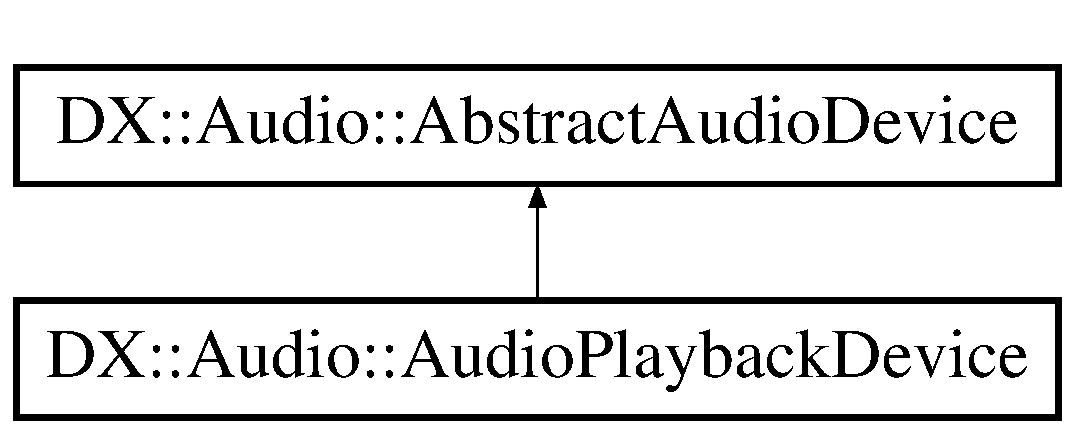
\includegraphics[height=2.000000cm]{class_d_x_1_1_audio_1_1_audio_playback_device}
\end{center}
\end{figure}
\subsection*{Public Member Functions}
\begin{DoxyCompactItemize}
\item 
\hypertarget{class_d_x_1_1_audio_1_1_audio_playback_device_aff876fcea4d589dd86c7189ddd270194}{virtual bool {\bfseries initialize} ()}\label{class_d_x_1_1_audio_1_1_audio_playback_device_aff876fcea4d589dd86c7189ddd270194}

\item 
\hypertarget{class_d_x_1_1_audio_1_1_audio_playback_device_af0fff74a1fa812045492a5971e21312d}{virtual bool {\bfseries is\-Playback\-Device} () const }\label{class_d_x_1_1_audio_1_1_audio_playback_device_af0fff74a1fa812045492a5971e21312d}

\item 
\hypertarget{class_d_x_1_1_audio_1_1_audio_playback_device_a70f4d9d97b78469ca0126635083acd1d}{virtual bool {\bfseries write\-To\-Buffer} (const \hyperlink{class_d_x_1_1_audio_1_1_audio_packet}{Audio\-Packet} \&in, const \hyperlink{struct_d_x_1_1_audio_1_1_abstract_filter}{Abstract\-Filter} \&filter)}\label{class_d_x_1_1_audio_1_1_audio_playback_device_a70f4d9d97b78469ca0126635083acd1d}

\item 
\hypertarget{class_d_x_1_1_audio_1_1_audio_playback_device_a53948a11de39e9e212038a9d9722e13a}{virtual bool {\bfseries write\-To\-Buffer} (\hyperlink{class_d_x_1_1_lock_free_1_1_concurrent_stream}{Audio\-Stream} \&in, const \hyperlink{struct_d_x_1_1_audio_1_1_abstract_filter}{Abstract\-Filter} \&filter, \hyperlink{class_d_x_1_1_audio_1_1_task_callback}{Task\-Callback} $\ast$callback=nullptr)}\label{class_d_x_1_1_audio_1_1_audio_playback_device_a53948a11de39e9e212038a9d9722e13a}

\item 
\hypertarget{class_d_x_1_1_audio_1_1_audio_playback_device_a58a266b68ccadceeb2e4a05ad2292973}{virtual \hyperlink{class_d_x_1_1_audio_1_1_audio_packet}{Audio\-Packet} {\bfseries read\-From\-Buffer} ()}\label{class_d_x_1_1_audio_1_1_audio_playback_device_a58a266b68ccadceeb2e4a05ad2292973}

\item 
\hypertarget{class_d_x_1_1_audio_1_1_audio_playback_device_a0279d91d609be8ae73d792712554dc16}{virtual bool {\bfseries read\-From\-Buffer} (\hyperlink{class_d_x_1_1_lock_free_1_1_concurrent_stream}{Audio\-Stream} \&out, \hyperlink{class_d_x_1_1_audio_1_1_task_callback}{Task\-Callback} $\ast$callback=nullptr)}\label{class_d_x_1_1_audio_1_1_audio_playback_device_a0279d91d609be8ae73d792712554dc16}

\end{DoxyCompactItemize}
\subsection*{Additional Inherited Members}


The documentation for this class was generated from the following files\-:\begin{DoxyCompactItemize}
\item 
Audio/Audio\-Playback\-Device.\-h\item 
Audio/Audio\-Playback\-Device.\-cpp\end{DoxyCompactItemize}

\hypertarget{class_d_x_1_1_audio_1_1_audio_sample}{\section{D\-X\-:\-:Audio\-:\-:Audio\-Sample Class Reference}
\label{class_d_x_1_1_audio_1_1_audio_sample}\index{D\-X\-::\-Audio\-::\-Audio\-Sample@{D\-X\-::\-Audio\-::\-Audio\-Sample}}
}


Audio\-Samples are byte packages of an individual sample of some audio waveform. The actual bitwise-\/makeup of any given sample is defined by an \hyperlink{struct_d_x_1_1_audio_1_1_audio_format}{Audio\-Format}. Audio\-Samples should {\itshape N\-E\-V\-E\-R} be orphaned from an \hyperlink{class_d_x_1_1_audio_1_1_audio_packet}{Audio\-Packet} -\/ they hold simple references to memory held by an \hyperlink{class_d_x_1_1_audio_1_1_audio_packet}{Audio\-Packet}, and have undefined (bad!) behavior if kept around past the lifetime of their parent \hyperlink{class_d_x_1_1_audio_1_1_audio_packet}{Audio\-Packet}.  




{\ttfamily \#include $<$Audio\-Packet.\-h$>$}

\subsection*{Public Member Functions}
\begin{DoxyCompactItemize}
\item 
\hyperlink{class_d_x_1_1_audio_1_1_audio_sample_ae8eb2486b80e7c7718a752ff738e8865}{Audio\-Sample} ()
\item 
\hyperlink{class_d_x_1_1_audio_1_1_audio_sample_afda761bd77a5dd23c198ada0c2ded88e}{Audio\-Sample} (const \hyperlink{struct_d_x_1_1_audio_1_1_audio_format}{Audio\-Format} \&format, Audio\-Byte $\ast$memory)
\item 
\hyperlink{class_d_x_1_1_audio_1_1_audio_sample_add0befe561a61667d7dc33bb9f41d311}{Audio\-Sample} (const \hyperlink{class_d_x_1_1_audio_1_1_audio_sample}{Audio\-Sample} \&copy)
\item 
\hyperlink{class_d_x_1_1_audio_1_1_audio_sample_adce1429f7e4e4aca198a7915a009efb2}{Audio\-Sample} (\hyperlink{class_d_x_1_1_audio_1_1_audio_sample}{Audio\-Sample} \&\&move)
\item 
\hyperlink{class_d_x_1_1_audio_1_1_audio_sample_a43cffccb172cda275cc68b1d9c6cfdb9}{$\sim$\-Audio\-Sample} ()
\item 
\hyperlink{class_d_x_1_1_audio_1_1_audio_sample}{Audio\-Sample} \& \hyperlink{class_d_x_1_1_audio_1_1_audio_sample_a7e54bfe2076f4f8c0f78616e015636e0}{operator=} (const \hyperlink{class_d_x_1_1_audio_1_1_audio_sample}{Audio\-Sample} \&copy)
\begin{DoxyCompactList}\small\item\em Copies the data that one sample points at to the \hyperlink{class_d_x_1_1_audio_1_1_audio_sample}{Audio\-Sample} defined by this. \end{DoxyCompactList}\end{DoxyCompactItemize}


\subsection{Detailed Description}
Audio\-Samples are byte packages of an individual sample of some audio waveform. The actual bitwise-\/makeup of any given sample is defined by an \hyperlink{struct_d_x_1_1_audio_1_1_audio_format}{Audio\-Format}. Audio\-Samples should {\itshape N\-E\-V\-E\-R} be orphaned from an \hyperlink{class_d_x_1_1_audio_1_1_audio_packet}{Audio\-Packet} -\/ they hold simple references to memory held by an \hyperlink{class_d_x_1_1_audio_1_1_audio_packet}{Audio\-Packet}, and have undefined (bad!) behavior if kept around past the lifetime of their parent \hyperlink{class_d_x_1_1_audio_1_1_audio_packet}{Audio\-Packet}. 

Audio\-Samples, for most cases, should never be directly accessed. Their primary purpose is to provide a nice abstraction for Filters (D\-S\-Ps) converting waveforms 

\subsection{Constructor \& Destructor Documentation}
\hypertarget{class_d_x_1_1_audio_1_1_audio_sample_ae8eb2486b80e7c7718a752ff738e8865}{\index{D\-X\-::\-Audio\-::\-Audio\-Sample@{D\-X\-::\-Audio\-::\-Audio\-Sample}!Audio\-Sample@{Audio\-Sample}}
\index{Audio\-Sample@{Audio\-Sample}!DX::Audio::AudioSample@{D\-X\-::\-Audio\-::\-Audio\-Sample}}
\subsubsection[{Audio\-Sample}]{\setlength{\rightskip}{0pt plus 5cm}D\-X\-::\-Audio\-::\-Audio\-Sample\-::\-Audio\-Sample (
\begin{DoxyParamCaption}
{}
\end{DoxyParamCaption}
)}}\label{class_d_x_1_1_audio_1_1_audio_sample_ae8eb2486b80e7c7718a752ff738e8865}
Default constructor, initializes empty \hyperlink{class_d_x_1_1_audio_1_1_audio_sample}{Audio\-Sample} \hypertarget{class_d_x_1_1_audio_1_1_audio_sample_afda761bd77a5dd23c198ada0c2ded88e}{\index{D\-X\-::\-Audio\-::\-Audio\-Sample@{D\-X\-::\-Audio\-::\-Audio\-Sample}!Audio\-Sample@{Audio\-Sample}}
\index{Audio\-Sample@{Audio\-Sample}!DX::Audio::AudioSample@{D\-X\-::\-Audio\-::\-Audio\-Sample}}
\subsubsection[{Audio\-Sample}]{\setlength{\rightskip}{0pt plus 5cm}D\-X\-::\-Audio\-::\-Audio\-Sample\-::\-Audio\-Sample (
\begin{DoxyParamCaption}
\item[{const {\bf Audio\-Format} \&}]{format, }
\item[{Audio\-Byte $\ast$}]{memory}
\end{DoxyParamCaption}
)}}\label{class_d_x_1_1_audio_1_1_audio_sample_afda761bd77a5dd23c198ada0c2ded88e}
Given an \hyperlink{struct_d_x_1_1_audio_1_1_audio_format}{Audio\-Format} and a pointer to some memory, outlines a single sample starting at at that point \hypertarget{class_d_x_1_1_audio_1_1_audio_sample_add0befe561a61667d7dc33bb9f41d311}{\index{D\-X\-::\-Audio\-::\-Audio\-Sample@{D\-X\-::\-Audio\-::\-Audio\-Sample}!Audio\-Sample@{Audio\-Sample}}
\index{Audio\-Sample@{Audio\-Sample}!DX::Audio::AudioSample@{D\-X\-::\-Audio\-::\-Audio\-Sample}}
\subsubsection[{Audio\-Sample}]{\setlength{\rightskip}{0pt plus 5cm}D\-X\-::\-Audio\-::\-Audio\-Sample\-::\-Audio\-Sample (
\begin{DoxyParamCaption}
\item[{const {\bf Audio\-Sample} \&}]{copy}
\end{DoxyParamCaption}
)}}\label{class_d_x_1_1_audio_1_1_audio_sample_add0befe561a61667d7dc33bb9f41d311}
Copy constructor, performs a shallow copy \hypertarget{class_d_x_1_1_audio_1_1_audio_sample_adce1429f7e4e4aca198a7915a009efb2}{\index{D\-X\-::\-Audio\-::\-Audio\-Sample@{D\-X\-::\-Audio\-::\-Audio\-Sample}!Audio\-Sample@{Audio\-Sample}}
\index{Audio\-Sample@{Audio\-Sample}!DX::Audio::AudioSample@{D\-X\-::\-Audio\-::\-Audio\-Sample}}
\subsubsection[{Audio\-Sample}]{\setlength{\rightskip}{0pt plus 5cm}D\-X\-::\-Audio\-::\-Audio\-Sample\-::\-Audio\-Sample (
\begin{DoxyParamCaption}
\item[{{\bf Audio\-Sample} \&\&}]{move}
\end{DoxyParamCaption}
)}}\label{class_d_x_1_1_audio_1_1_audio_sample_adce1429f7e4e4aca198a7915a009efb2}
Move constructor, should not invalidate move's data \hypertarget{class_d_x_1_1_audio_1_1_audio_sample_a43cffccb172cda275cc68b1d9c6cfdb9}{\index{D\-X\-::\-Audio\-::\-Audio\-Sample@{D\-X\-::\-Audio\-::\-Audio\-Sample}!$\sim$\-Audio\-Sample@{$\sim$\-Audio\-Sample}}
\index{$\sim$\-Audio\-Sample@{$\sim$\-Audio\-Sample}!DX::Audio::AudioSample@{D\-X\-::\-Audio\-::\-Audio\-Sample}}
\subsubsection[{$\sim$\-Audio\-Sample}]{\setlength{\rightskip}{0pt plus 5cm}D\-X\-::\-Audio\-::\-Audio\-Sample\-::$\sim$\-Audio\-Sample (
\begin{DoxyParamCaption}
{}
\end{DoxyParamCaption}
)}}\label{class_d_x_1_1_audio_1_1_audio_sample_a43cffccb172cda275cc68b1d9c6cfdb9}
Does N\-O\-T clean up memory 

\subsection{Member Function Documentation}
\hypertarget{class_d_x_1_1_audio_1_1_audio_sample_a7e54bfe2076f4f8c0f78616e015636e0}{\index{D\-X\-::\-Audio\-::\-Audio\-Sample@{D\-X\-::\-Audio\-::\-Audio\-Sample}!operator=@{operator=}}
\index{operator=@{operator=}!DX::Audio::AudioSample@{D\-X\-::\-Audio\-::\-Audio\-Sample}}
\subsubsection[{operator=}]{\setlength{\rightskip}{0pt plus 5cm}{\bf Audio\-Sample} \& D\-X\-::\-Audio\-::\-Audio\-Sample\-::operator= (
\begin{DoxyParamCaption}
\item[{const {\bf Audio\-Sample} \&}]{copy}
\end{DoxyParamCaption}
)}}\label{class_d_x_1_1_audio_1_1_audio_sample_a7e54bfe2076f4f8c0f78616e015636e0}


Copies the data that one sample points at to the \hyperlink{class_d_x_1_1_audio_1_1_audio_sample}{Audio\-Sample} defined by this. 

\begin{DoxyNote}{Note}
This is the only method that Audio\-Samples have that allows for memory modification. 

This method D\-O\-E\-S N\-O\-T P\-E\-R\-F\-O\-R\-M A\-N\-Y T\-R\-A\-N\-S\-F\-O\-R\-M\-S. If the channels \& bits\-Per\-Sample of the corresponding Audio\-Samples do not align, then this will result in B\-A\-D D\-A\-T\-A 
\end{DoxyNote}


The documentation for this class was generated from the following files\-:\begin{DoxyCompactItemize}
\item 
Audio/Audio\-Packet.\-h\item 
Audio/Audio\-Packet.\-cpp\end{DoxyCompactItemize}

\hypertarget{class_d_x_1_1_lock_free_1_1_concurrent_queue}{\section{D\-X\-:\-:Lock\-Free\-:\-:Concurrent\-Queue$<$ T $>$ Class Template Reference}
\label{class_d_x_1_1_lock_free_1_1_concurrent_queue}\index{D\-X\-::\-Lock\-Free\-::\-Concurrent\-Queue$<$ T $>$@{D\-X\-::\-Lock\-Free\-::\-Concurrent\-Queue$<$ T $>$}}
}
Inheritance diagram for D\-X\-:\-:Lock\-Free\-:\-:Concurrent\-Queue$<$ T $>$\-:\begin{figure}[H]
\begin{center}
\leavevmode
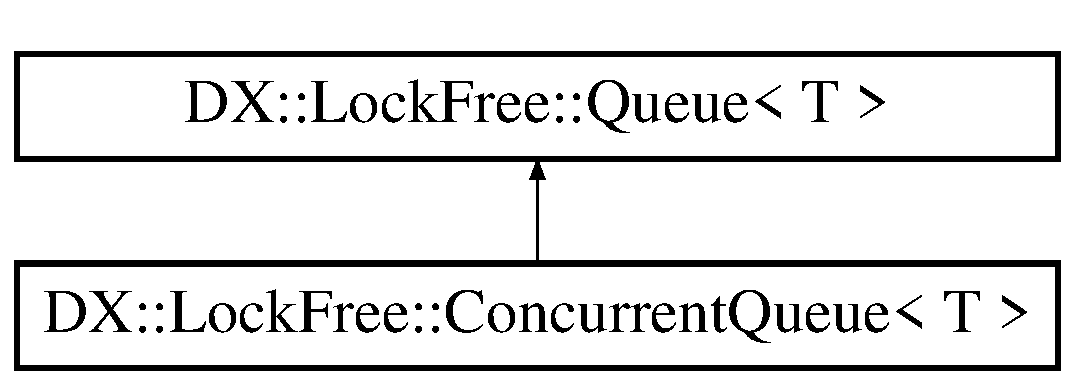
\includegraphics[height=2.000000cm]{class_d_x_1_1_lock_free_1_1_concurrent_queue}
\end{center}
\end{figure}
\subsection*{Public Member Functions}
\begin{DoxyCompactItemize}
\item 
\hypertarget{class_d_x_1_1_lock_free_1_1_concurrent_queue_a489a668b3ead8e118342cd496b90fdc3}{{\bfseries Concurrent\-Queue} (const \hyperlink{class_d_x_1_1_lock_free_1_1_concurrent_queue}{Concurrent\-Queue} \&copy)}\label{class_d_x_1_1_lock_free_1_1_concurrent_queue_a489a668b3ead8e118342cd496b90fdc3}

\item 
\hypertarget{class_d_x_1_1_lock_free_1_1_concurrent_queue_a581d154f54650724c479edbcfcbd86ec}{{\bfseries Concurrent\-Queue} (\hyperlink{class_d_x_1_1_lock_free_1_1_concurrent_queue}{Concurrent\-Queue} \&\&move)}\label{class_d_x_1_1_lock_free_1_1_concurrent_queue_a581d154f54650724c479edbcfcbd86ec}

\item 
\hypertarget{class_d_x_1_1_lock_free_1_1_concurrent_queue_ad2091be06f9ff988e720e8dcf6892d26}{bool {\bfseries is\-Empty} () const }\label{class_d_x_1_1_lock_free_1_1_concurrent_queue_ad2091be06f9ff988e720e8dcf6892d26}

\item 
\hypertarget{class_d_x_1_1_lock_free_1_1_concurrent_queue_af41b589534d1513556ea179b5d2b1e84}{size\-\_\-t {\bfseries size} () const }\label{class_d_x_1_1_lock_free_1_1_concurrent_queue_af41b589534d1513556ea179b5d2b1e84}

\item 
\hypertarget{class_d_x_1_1_lock_free_1_1_concurrent_queue_a918c26bab246dbbaef94866f5c20fa3a}{bool {\bfseries front} (T \&out) const }\label{class_d_x_1_1_lock_free_1_1_concurrent_queue_a918c26bab246dbbaef94866f5c20fa3a}

\item 
\hypertarget{class_d_x_1_1_lock_free_1_1_concurrent_queue_ac9e79362ce3b1b30655ce1104ef3e39b}{bool {\bfseries pop} (T \&out)}\label{class_d_x_1_1_lock_free_1_1_concurrent_queue_ac9e79362ce3b1b30655ce1104ef3e39b}

\item 
\hypertarget{class_d_x_1_1_lock_free_1_1_concurrent_queue_a8612ba2519138505ea0dd158816194b9}{void {\bfseries push} (const T \&in)}\label{class_d_x_1_1_lock_free_1_1_concurrent_queue_a8612ba2519138505ea0dd158816194b9}

\item 
\hypertarget{class_d_x_1_1_lock_free_1_1_concurrent_queue_aaead004ad8fe7db381bff7c09c9f221c}{void {\bfseries push} (T \&\&move\-In)}\label{class_d_x_1_1_lock_free_1_1_concurrent_queue_aaead004ad8fe7db381bff7c09c9f221c}

\item 
\hypertarget{class_d_x_1_1_lock_free_1_1_concurrent_queue_a03b5624a1621065696ca49482bc59dce}{void {\bfseries clear} ()}\label{class_d_x_1_1_lock_free_1_1_concurrent_queue_a03b5624a1621065696ca49482bc59dce}

\end{DoxyCompactItemize}
\subsection*{Additional Inherited Members}


The documentation for this class was generated from the following file\-:\begin{DoxyCompactItemize}
\item 
Lock\-Free/\-Containers/Concurrent\-Queue.\-h\end{DoxyCompactItemize}

\hypertarget{class_d_x_1_1_lock_free_1_1_concurrent_stream}{\section{D\-X\-:\-:Lock\-Free\-:\-:Concurrent\-Stream$<$ T $>$ Class Template Reference}
\label{class_d_x_1_1_lock_free_1_1_concurrent_stream}\index{D\-X\-::\-Lock\-Free\-::\-Concurrent\-Stream$<$ T $>$@{D\-X\-::\-Lock\-Free\-::\-Concurrent\-Stream$<$ T $>$}}
}
Inheritance diagram for D\-X\-:\-:Lock\-Free\-:\-:Concurrent\-Stream$<$ T $>$\-:\begin{figure}[H]
\begin{center}
\leavevmode
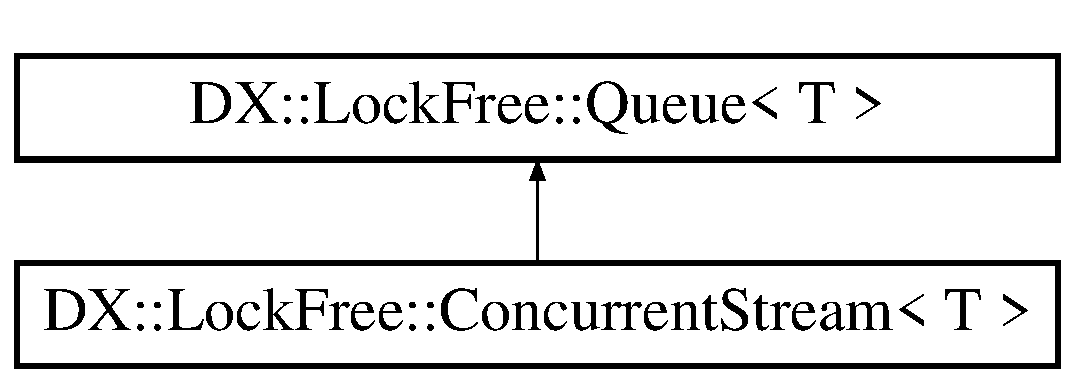
\includegraphics[height=2.000000cm]{class_d_x_1_1_lock_free_1_1_concurrent_stream}
\end{center}
\end{figure}
\subsection*{Public Member Functions}
\begin{DoxyCompactItemize}
\item 
\hypertarget{class_d_x_1_1_lock_free_1_1_concurrent_stream_a5e9ee519ec757e4fa5e87df6aa466bc1}{{\bfseries Concurrent\-Stream} (const \hyperlink{class_d_x_1_1_lock_free_1_1_concurrent_stream}{Concurrent\-Stream} \&)}\label{class_d_x_1_1_lock_free_1_1_concurrent_stream_a5e9ee519ec757e4fa5e87df6aa466bc1}

\item 
\hypertarget{class_d_x_1_1_lock_free_1_1_concurrent_stream_a3deff0f2eb5ea3e9c3388c4fa52f9b85}{{\bfseries Concurrent\-Stream} (\hyperlink{class_d_x_1_1_lock_free_1_1_concurrent_stream}{Concurrent\-Stream} \&\&)}\label{class_d_x_1_1_lock_free_1_1_concurrent_stream_a3deff0f2eb5ea3e9c3388c4fa52f9b85}

\item 
\hypertarget{class_d_x_1_1_lock_free_1_1_concurrent_stream_aed04a552a34567af1d8fb878ee45c560}{bool {\bfseries is\-Empty} () const }\label{class_d_x_1_1_lock_free_1_1_concurrent_stream_aed04a552a34567af1d8fb878ee45c560}

\item 
\hypertarget{class_d_x_1_1_lock_free_1_1_concurrent_stream_a320844912e423dfb318ba91335ac25f6}{size\-\_\-t {\bfseries size} () const }\label{class_d_x_1_1_lock_free_1_1_concurrent_stream_a320844912e423dfb318ba91335ac25f6}

\item 
\hypertarget{class_d_x_1_1_lock_free_1_1_concurrent_stream_aa0205ac58036a4f24338be5203e4401c}{bool {\bfseries front} (T \&out) const }\label{class_d_x_1_1_lock_free_1_1_concurrent_stream_aa0205ac58036a4f24338be5203e4401c}

\item 
\hypertarget{class_d_x_1_1_lock_free_1_1_concurrent_stream_afb5efcb0b628590c44fa837cdb5ab2ae}{bool {\bfseries pop} (T \&out)}\label{class_d_x_1_1_lock_free_1_1_concurrent_stream_afb5efcb0b628590c44fa837cdb5ab2ae}

\item 
\hypertarget{class_d_x_1_1_lock_free_1_1_concurrent_stream_ac4c611d386c3de1f6831208f61bb9c33}{void {\bfseries push} (const T \&in)}\label{class_d_x_1_1_lock_free_1_1_concurrent_stream_ac4c611d386c3de1f6831208f61bb9c33}

\item 
\hypertarget{class_d_x_1_1_lock_free_1_1_concurrent_stream_a3f554a07f630e9d3f39ca99bcd46a952}{void {\bfseries push} (T \&\&move\-In)}\label{class_d_x_1_1_lock_free_1_1_concurrent_stream_a3f554a07f630e9d3f39ca99bcd46a952}

\item 
\hypertarget{class_d_x_1_1_lock_free_1_1_concurrent_stream_aa137361af8ac8f1691d76ff2e3f227cc}{void {\bfseries clear} ()}\label{class_d_x_1_1_lock_free_1_1_concurrent_stream_aa137361af8ac8f1691d76ff2e3f227cc}

\end{DoxyCompactItemize}
\subsection*{Additional Inherited Members}


The documentation for this class was generated from the following file\-:\begin{DoxyCompactItemize}
\item 
Lock\-Free/\-Containers/Concurrent\-Stream.\-h\end{DoxyCompactItemize}

\hypertarget{class_d_x_1_1_lock_free_1_1_cyclic_spin_barrier}{\section{D\-X\-:\-:Lock\-Free\-:\-:Cyclic\-Spin\-Barrier Class Reference}
\label{class_d_x_1_1_lock_free_1_1_cyclic_spin_barrier}\index{D\-X\-::\-Lock\-Free\-::\-Cyclic\-Spin\-Barrier@{D\-X\-::\-Lock\-Free\-::\-Cyclic\-Spin\-Barrier}}
}


\hyperlink{class_d_x_1_1_lock_free_1_1_cyclic_spin_barrier}{Cyclic\-Spin\-Barrier} is an \hyperlink{class_d_x_1_1_lock_free_1_1_abstract_barrier}{Abstract\-Barrier} implementation that will reset itself after all calls to \hyperlink{class_d_x_1_1_lock_free_1_1_cyclic_spin_barrier_af9b42b0455c7251bda38694a2df17d11}{wait()} have unblocked. This allows for barrier use within loops that require blocking at the end, or other similar scenarios.  




{\ttfamily \#include $<$Cyclic\-Spin\-Barrier.\-h$>$}

Inheritance diagram for D\-X\-:\-:Lock\-Free\-:\-:Cyclic\-Spin\-Barrier\-:\begin{figure}[H]
\begin{center}
\leavevmode
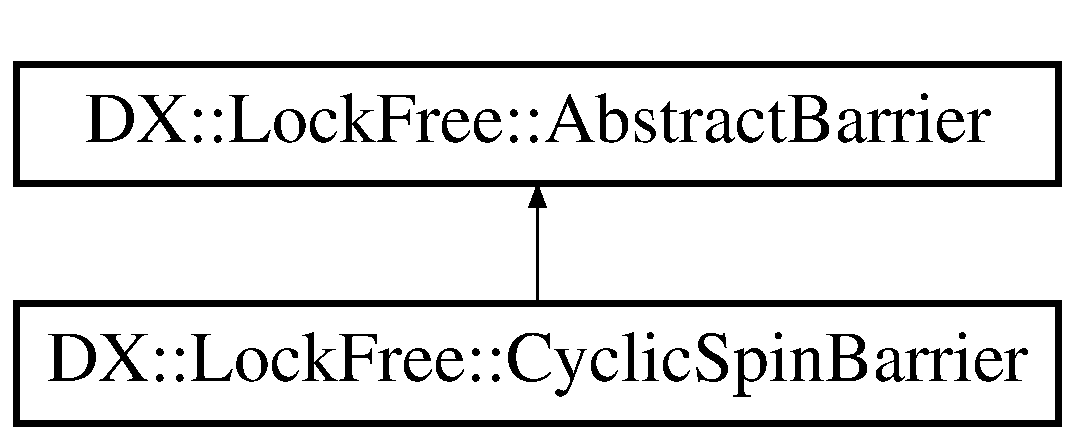
\includegraphics[height=2.000000cm]{class_d_x_1_1_lock_free_1_1_cyclic_spin_barrier}
\end{center}
\end{figure}
\subsection*{Public Member Functions}
\begin{DoxyCompactItemize}
\item 
\hyperlink{class_d_x_1_1_lock_free_1_1_cyclic_spin_barrier_a857ff57e8576bee333452b0f3f3f1515}{Cyclic\-Spin\-Barrier} (size\-\_\-t num\-Threads=2)
\item 
void \hyperlink{class_d_x_1_1_lock_free_1_1_cyclic_spin_barrier_af9b42b0455c7251bda38694a2df17d11}{wait} () const 
\end{DoxyCompactItemize}
\subsection*{Additional Inherited Members}


\subsection{Detailed Description}
\hyperlink{class_d_x_1_1_lock_free_1_1_cyclic_spin_barrier}{Cyclic\-Spin\-Barrier} is an \hyperlink{class_d_x_1_1_lock_free_1_1_abstract_barrier}{Abstract\-Barrier} implementation that will reset itself after all calls to \hyperlink{class_d_x_1_1_lock_free_1_1_cyclic_spin_barrier_af9b42b0455c7251bda38694a2df17d11}{wait()} have unblocked. This allows for barrier use within loops that require blocking at the end, or other similar scenarios. 


\begin{DoxyCode}
\textcolor{keywordtype}{void} process(\hyperlink{class_d_x_1_1_lock_free_1_1_cyclic_spin_barrier_a857ff57e8576bee333452b0f3f3f1515}{CyclicSpinBarrier}& barrier1, \hyperlink{class_d_x_1_1_lock_free_1_1_cyclic_spin_barrier_a857ff57e8576bee333452b0f3f3f1515}{CyclicSpinBarrier}& barrier2)
\{
    \textcolor{keywordflow}{while}(\textcolor{keyword}{true})
    \{
        \textcolor{comment}{// Do some work}
        barrier1.wait();
        barrier2.wait();
    \}
\}

\textcolor{keywordtype}{int} main(\textcolor{keywordtype}{int} argc, \textcolor{keywordtype}{char}* argv[])
\{
    \hyperlink{class_d_x_1_1_lock_free_1_1_cyclic_spin_barrier_a857ff57e8576bee333452b0f3f3f1515}{CyclicSpinBarrier} innerBarrier(5);
    \hyperlink{class_d_x_1_1_lock_free_1_1_cyclic_spin_barrier_a857ff57e8576bee333452b0f3f3f1515}{CyclicSpinBarrier} outerBarrier(5);

    \textcolor{keywordflow}{for}(\textcolor{keywordtype}{int} i = 0; i < 4; ++i)
        std::thread(&process, innerBarrier, outerBarrier);

    \textcolor{keywordflow}{while}(\textcolor{keyword}{true})
    \{
        barrier1.wait();
        \textcolor{comment}{// Here, work has completed in all threads for the current loop}
        \textcolor{comment}{// Do something synchronous with the work}
        barrier2.wait();    \textcolor{comment}{// Allows all threads to continue looping}
    \}

    \textcolor{keywordflow}{return} 0;        
\}
\end{DoxyCode}
 

\subsection{Constructor \& Destructor Documentation}
\hypertarget{class_d_x_1_1_lock_free_1_1_cyclic_spin_barrier_a857ff57e8576bee333452b0f3f3f1515}{\index{D\-X\-::\-Lock\-Free\-::\-Cyclic\-Spin\-Barrier@{D\-X\-::\-Lock\-Free\-::\-Cyclic\-Spin\-Barrier}!Cyclic\-Spin\-Barrier@{Cyclic\-Spin\-Barrier}}
\index{Cyclic\-Spin\-Barrier@{Cyclic\-Spin\-Barrier}!DX::LockFree::CyclicSpinBarrier@{D\-X\-::\-Lock\-Free\-::\-Cyclic\-Spin\-Barrier}}
\subsubsection[{Cyclic\-Spin\-Barrier}]{\setlength{\rightskip}{0pt plus 5cm}D\-X\-::\-Lock\-Free\-::\-Cyclic\-Spin\-Barrier\-::\-Cyclic\-Spin\-Barrier (
\begin{DoxyParamCaption}
\item[{size\-\_\-t}]{num\-Threads = {\ttfamily 2}}
\end{DoxyParamCaption}
)}}\label{class_d_x_1_1_lock_free_1_1_cyclic_spin_barrier_a857ff57e8576bee333452b0f3f3f1515}
Constructs a Cyclic\-Spinbarrier with a number of threads to wait on. This number defaults to 2, so Cyclic\-Spinbarriers can be constructed by calling\-: 
\begin{DoxyCode}
\hyperlink{class_d_x_1_1_lock_free_1_1_cyclic_spin_barrier_a857ff57e8576bee333452b0f3f3f1515}{CyclicSpinBarrier}();
\end{DoxyCode}


Although this is not recommended. 

\subsection{Member Function Documentation}
\hypertarget{class_d_x_1_1_lock_free_1_1_cyclic_spin_barrier_af9b42b0455c7251bda38694a2df17d11}{\index{D\-X\-::\-Lock\-Free\-::\-Cyclic\-Spin\-Barrier@{D\-X\-::\-Lock\-Free\-::\-Cyclic\-Spin\-Barrier}!wait@{wait}}
\index{wait@{wait}!DX::LockFree::CyclicSpinBarrier@{D\-X\-::\-Lock\-Free\-::\-Cyclic\-Spin\-Barrier}}
\subsubsection[{wait}]{\setlength{\rightskip}{0pt plus 5cm}void D\-X\-::\-Lock\-Free\-::\-Cyclic\-Spin\-Barrier\-::wait (
\begin{DoxyParamCaption}
{}
\end{DoxyParamCaption}
) const\hspace{0.3cm}{\ttfamily [virtual]}}}\label{class_d_x_1_1_lock_free_1_1_cyclic_spin_barrier_af9b42b0455c7251bda38694a2df17d11}
Blocks the current thread of execution until all other \hyperlink{class_d_x_1_1_lock_free_1_1_cyclic_spin_barrier_af9b42b0455c7251bda38694a2df17d11}{wait()} calls have beem made 

Implements \hyperlink{class_d_x_1_1_lock_free_1_1_abstract_barrier_a9040adf7507467e5a653bdaf2fbd17a6}{D\-X\-::\-Lock\-Free\-::\-Abstract\-Barrier}.



The documentation for this class was generated from the following files\-:\begin{DoxyCompactItemize}
\item 
Lock\-Free/\-Mutex/Cyclic\-Spin\-Barrier.\-h\item 
Lock\-Free/\-Mutex/Cyclic\-Spin\-Barrier.\-cpp\end{DoxyCompactItemize}

\hypertarget{class_d_x_1_1_lock_free_1_1_mutex}{\section{D\-X\-:\-:Lock\-Free\-:\-:Mutex Class Reference}
\label{class_d_x_1_1_lock_free_1_1_mutex}\index{D\-X\-::\-Lock\-Free\-::\-Mutex@{D\-X\-::\-Lock\-Free\-::\-Mutex}}
}


\hyperlink{class_d_x_1_1_lock_free_1_1_mutex}{Mutex} is a general descriptor for a class of objects that perform analagous to actual Mutexes. However, their exact implementations and yielding behavior may vary.  




{\ttfamily \#include $<$Mutex.\-h$>$}

Inheritance diagram for D\-X\-:\-:Lock\-Free\-:\-:Mutex\-:\begin{figure}[H]
\begin{center}
\leavevmode
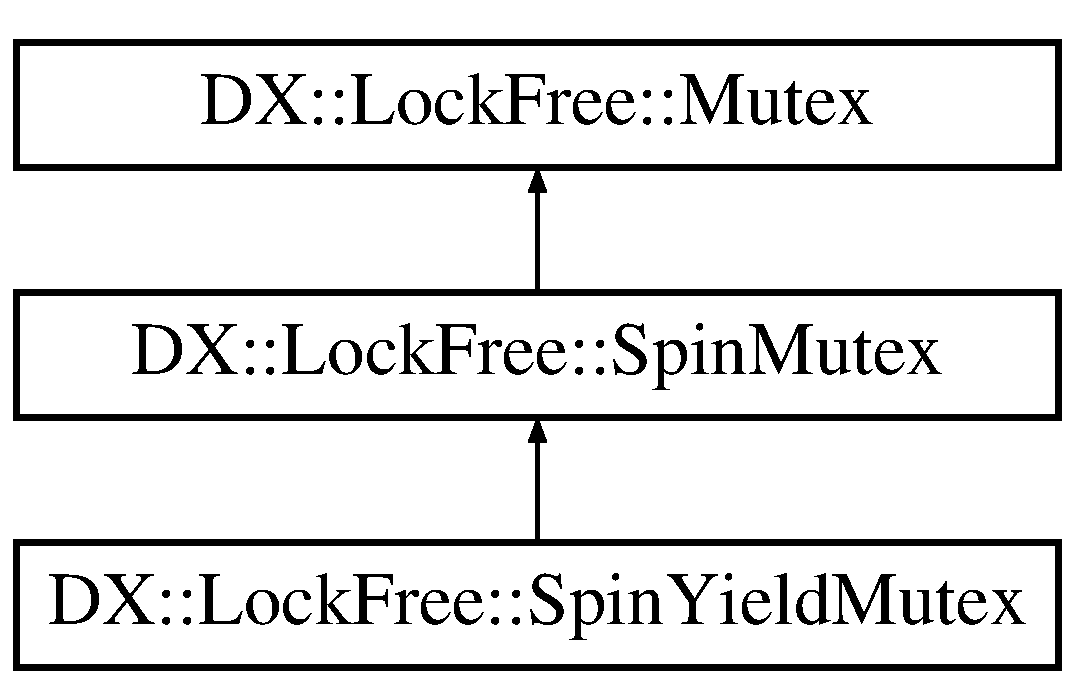
\includegraphics[height=3.000000cm]{class_d_x_1_1_lock_free_1_1_mutex}
\end{center}
\end{figure}
\subsection*{Public Member Functions}
\begin{DoxyCompactItemize}
\item 
\hypertarget{class_d_x_1_1_lock_free_1_1_mutex_acf5c8caa6a556b29df4ed345f6cd0858}{virtual void {\bfseries lock} () const =0}\label{class_d_x_1_1_lock_free_1_1_mutex_acf5c8caa6a556b29df4ed345f6cd0858}

\item 
\hypertarget{class_d_x_1_1_lock_free_1_1_mutex_a4975ec604dfd57bf96cd1f374ce3f2a3}{virtual void {\bfseries unlock} () const =0}\label{class_d_x_1_1_lock_free_1_1_mutex_a4975ec604dfd57bf96cd1f374ce3f2a3}

\end{DoxyCompactItemize}


\subsection{Detailed Description}
\hyperlink{class_d_x_1_1_lock_free_1_1_mutex}{Mutex} is a general descriptor for a class of objects that perform analagous to actual Mutexes. However, their exact implementations and yielding behavior may vary. 

The documentation for this class was generated from the following files\-:\begin{DoxyCompactItemize}
\item 
Lock\-Free/\-Mutex/Mutex.\-h\item 
Lock\-Free/\-Mutex/Mutex.\-cpp\end{DoxyCompactItemize}

\hypertarget{struct_d_x_1_1_lock_free_1_1_node}{\section{D\-X\-:\-:Lock\-Free\-:\-:Node$<$ T $>$ Struct Template Reference}
\label{struct_d_x_1_1_lock_free_1_1_node}\index{D\-X\-::\-Lock\-Free\-::\-Node$<$ T $>$@{D\-X\-::\-Lock\-Free\-::\-Node$<$ T $>$}}
}
\subsection*{Public Member Functions}
\begin{DoxyCompactItemize}
\item 
\hypertarget{struct_d_x_1_1_lock_free_1_1_node_a2de3380e5423dc3d4edf17b33e1c4945}{{\bfseries Node} (T $\ast$data)}\label{struct_d_x_1_1_lock_free_1_1_node_a2de3380e5423dc3d4edf17b33e1c4945}

\end{DoxyCompactItemize}
\subsection*{Public Attributes}
\begin{DoxyCompactItemize}
\item 
\hypertarget{struct_d_x_1_1_lock_free_1_1_node_a42c6086397b8cbdecbc50095646d3b05}{T $\ast$ {\bfseries data}}\label{struct_d_x_1_1_lock_free_1_1_node_a42c6086397b8cbdecbc50095646d3b05}

\item 
\hypertarget{struct_d_x_1_1_lock_free_1_1_node_a8e86040f2e9bee28a7a736559cce086c}{std\-::atomic$<$ \hyperlink{struct_d_x_1_1_lock_free_1_1_node}{Node} $\ast$ $>$ {\bfseries next}}\label{struct_d_x_1_1_lock_free_1_1_node_a8e86040f2e9bee28a7a736559cce086c}

\item 
\hypertarget{struct_d_x_1_1_lock_free_1_1_node_a5773af1ce0c200ba7aa747b351b99bf4}{volatile char {\bfseries pad\-\_\-} \mbox{[}C\-A\-C\-H\-E\-\_\-\-L\-I\-N\-E\-\_\-\-S\-I\-Z\-E-\/((sizeof(T $\ast$)+sizeof(std\-::atomic$<$ \hyperlink{struct_d_x_1_1_lock_free_1_1_node}{Node} $\ast$ $>$))\%C\-A\-C\-H\-E\-\_\-\-L\-I\-N\-E\-\_\-\-S\-I\-Z\-E)\mbox{]}}\label{struct_d_x_1_1_lock_free_1_1_node_a5773af1ce0c200ba7aa747b351b99bf4}

\end{DoxyCompactItemize}


The documentation for this struct was generated from the following file\-:\begin{DoxyCompactItemize}
\item 
Lock\-Free/\-Containers/Abstract\-Queue.\-h\end{DoxyCompactItemize}

\hypertarget{class_d_x_1_1_lock_free_1_1_queue}{\section{D\-X\-:\-:Lock\-Free\-:\-:Queue$<$ T $>$ Class Template Reference}
\label{class_d_x_1_1_lock_free_1_1_queue}\index{D\-X\-::\-Lock\-Free\-::\-Queue$<$ T $>$@{D\-X\-::\-Lock\-Free\-::\-Queue$<$ T $>$}}
}
Inheritance diagram for D\-X\-:\-:Lock\-Free\-:\-:Queue$<$ T $>$\-:\begin{figure}[H]
\begin{center}
\leavevmode
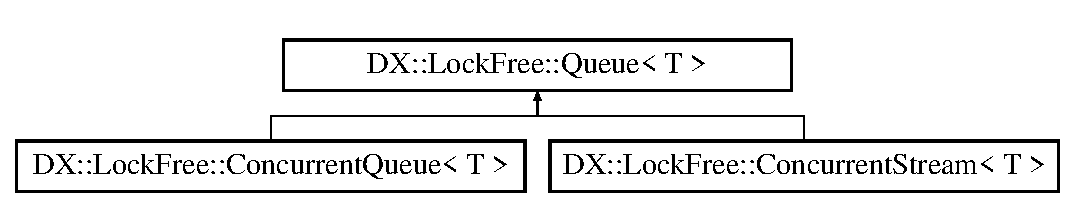
\includegraphics[height=2.000000cm]{class_d_x_1_1_lock_free_1_1_queue}
\end{center}
\end{figure}
\subsection*{Public Member Functions}
\begin{DoxyCompactItemize}
\item 
\hypertarget{class_d_x_1_1_lock_free_1_1_queue_af66e7cba57d219d81608c24eb5e397d5}{virtual bool {\bfseries is\-Empty} () const }\label{class_d_x_1_1_lock_free_1_1_queue_af66e7cba57d219d81608c24eb5e397d5}

\item 
\hypertarget{class_d_x_1_1_lock_free_1_1_queue_ac28a6a1ff587e5005bd97d6c159533ed}{virtual size\-\_\-t {\bfseries size} () const }\label{class_d_x_1_1_lock_free_1_1_queue_ac28a6a1ff587e5005bd97d6c159533ed}

\item 
\hypertarget{class_d_x_1_1_lock_free_1_1_queue_a6e392d698cefc4b01ed27154a18524af}{virtual bool {\bfseries front} (T \&out) const =0}\label{class_d_x_1_1_lock_free_1_1_queue_a6e392d698cefc4b01ed27154a18524af}

\item 
\hypertarget{class_d_x_1_1_lock_free_1_1_queue_a10af88de439fbcd64e675907640533cd}{virtual bool {\bfseries pop} (T \&in)=0}\label{class_d_x_1_1_lock_free_1_1_queue_a10af88de439fbcd64e675907640533cd}

\item 
\hypertarget{class_d_x_1_1_lock_free_1_1_queue_aba6b10fa9f6d36fae16776ce7984009c}{virtual void {\bfseries push} (const T \&in)=0}\label{class_d_x_1_1_lock_free_1_1_queue_aba6b10fa9f6d36fae16776ce7984009c}

\item 
\hypertarget{class_d_x_1_1_lock_free_1_1_queue_adeb07374710138df3b5d28bddb8974ea}{virtual void {\bfseries push} (T \&\&in)=0}\label{class_d_x_1_1_lock_free_1_1_queue_adeb07374710138df3b5d28bddb8974ea}

\item 
\hypertarget{class_d_x_1_1_lock_free_1_1_queue_aedf62168879b92f0e269d2f1fba4c93a}{virtual void {\bfseries clear} ()=0}\label{class_d_x_1_1_lock_free_1_1_queue_aedf62168879b92f0e269d2f1fba4c93a}

\item 
\hypertarget{class_d_x_1_1_lock_free_1_1_queue_af83dc0f90f3534811f3057db384d58a8}{bool {\bfseries operator$>$$>$} (T \&)}\label{class_d_x_1_1_lock_free_1_1_queue_af83dc0f90f3534811f3057db384d58a8}

\item 
\hypertarget{class_d_x_1_1_lock_free_1_1_queue_ace553782c66d594008cc0e26f588f9cf}{\hyperlink{class_d_x_1_1_lock_free_1_1_queue}{Queue} \& {\bfseries operator$<$$<$} (const T \&)}\label{class_d_x_1_1_lock_free_1_1_queue_ace553782c66d594008cc0e26f588f9cf}

\end{DoxyCompactItemize}
\subsection*{Protected Attributes}
\begin{DoxyCompactItemize}
\item 
\hypertarget{class_d_x_1_1_lock_free_1_1_queue_afd72533778860258f3cedb4a2a6b6a17}{\hyperlink{struct_d_x_1_1_lock_free_1_1_node}{Node}$<$ T $>$ $\ast$ {\bfseries m\-\_\-start}}\label{class_d_x_1_1_lock_free_1_1_queue_afd72533778860258f3cedb4a2a6b6a17}

\item 
\hypertarget{class_d_x_1_1_lock_free_1_1_queue_a69296c6b2dbdc10eca9ce91c5c5e8696}{volatile char {\bfseries pad\-\_\-0} \mbox{[}C\-A\-C\-H\-E\-\_\-\-L\-I\-N\-E\-\_\-\-S\-I\-Z\-E-\/(sizeof(\hyperlink{struct_d_x_1_1_lock_free_1_1_node}{Node}$<$ T $>$ $\ast$)\%C\-A\-C\-H\-E\-\_\-\-L\-I\-N\-E\-\_\-\-S\-I\-Z\-E)\mbox{]}}\label{class_d_x_1_1_lock_free_1_1_queue_a69296c6b2dbdc10eca9ce91c5c5e8696}

\item 
\hypertarget{class_d_x_1_1_lock_free_1_1_queue_a8e4a95ccaa9cdd92b29ee10ebd3dbe9d}{\hyperlink{struct_d_x_1_1_lock_free_1_1_node}{Node}$<$ T $>$ $\ast$ {\bfseries m\-\_\-end}}\label{class_d_x_1_1_lock_free_1_1_queue_a8e4a95ccaa9cdd92b29ee10ebd3dbe9d}

\item 
\hypertarget{class_d_x_1_1_lock_free_1_1_queue_a97abcd8082dd19a63ead25ef8697a92d}{volatile char {\bfseries pad\-\_\-1} \mbox{[}C\-A\-C\-H\-E\-\_\-\-L\-I\-N\-E\-\_\-\-S\-I\-Z\-E-\/(sizeof(\hyperlink{struct_d_x_1_1_lock_free_1_1_node}{Node}$<$ T $>$ $\ast$)\%C\-A\-C\-H\-E\-\_\-\-L\-I\-N\-E\-\_\-\-S\-I\-Z\-E)\mbox{]}}\label{class_d_x_1_1_lock_free_1_1_queue_a97abcd8082dd19a63ead25ef8697a92d}

\item 
\hypertarget{class_d_x_1_1_lock_free_1_1_queue_a1cf52809012fae94ab715590803ddcd2}{std\-::atomic$<$ size\-\_\-t $>$ {\bfseries m\-\_\-size}}\label{class_d_x_1_1_lock_free_1_1_queue_a1cf52809012fae94ab715590803ddcd2}

\item 
\hypertarget{class_d_x_1_1_lock_free_1_1_queue_ae736270ff54ecf46a650a2399551665a}{volatile char {\bfseries pad\-\_\-2} \mbox{[}C\-A\-C\-H\-E\-\_\-\-L\-I\-N\-E\-\_\-\-S\-I\-Z\-E-\/(sizeof(std\-::atomic$<$ size\-\_\-t $>$)\%C\-A\-C\-H\-E\-\_\-\-L\-I\-N\-E\-\_\-\-S\-I\-Z\-E)\mbox{]}}\label{class_d_x_1_1_lock_free_1_1_queue_ae736270ff54ecf46a650a2399551665a}

\end{DoxyCompactItemize}


The documentation for this class was generated from the following file\-:\begin{DoxyCompactItemize}
\item 
Lock\-Free/\-Containers/Abstract\-Queue.\-h\end{DoxyCompactItemize}

\hypertarget{class_d_x_1_1_lock_free_1_1_r_w_mutex}{\section{D\-X\-:\-:Lock\-Free\-:\-:R\-W\-Mutex Class Reference}
\label{class_d_x_1_1_lock_free_1_1_r_w_mutex}\index{D\-X\-::\-Lock\-Free\-::\-R\-W\-Mutex@{D\-X\-::\-Lock\-Free\-::\-R\-W\-Mutex}}
}


\hyperlink{class_d_x_1_1_lock_free_1_1_r_w_mutex}{R\-W\-Mutex} is a general descriptor for a class of mutex-\/like objects that support multiple readers or a single writer. Unlike their \hyperlink{class_d_x_1_1_lock_free_1_1_mutex}{Mutex} counterparts, R\-W\-Mutexes have two different lock() and unlock() methods -\/ one set for writers and one set for readers.  




{\ttfamily \#include $<$R\-W\-Mutex.\-h$>$}

Inheritance diagram for D\-X\-:\-:Lock\-Free\-:\-:R\-W\-Mutex\-:\begin{figure}[H]
\begin{center}
\leavevmode
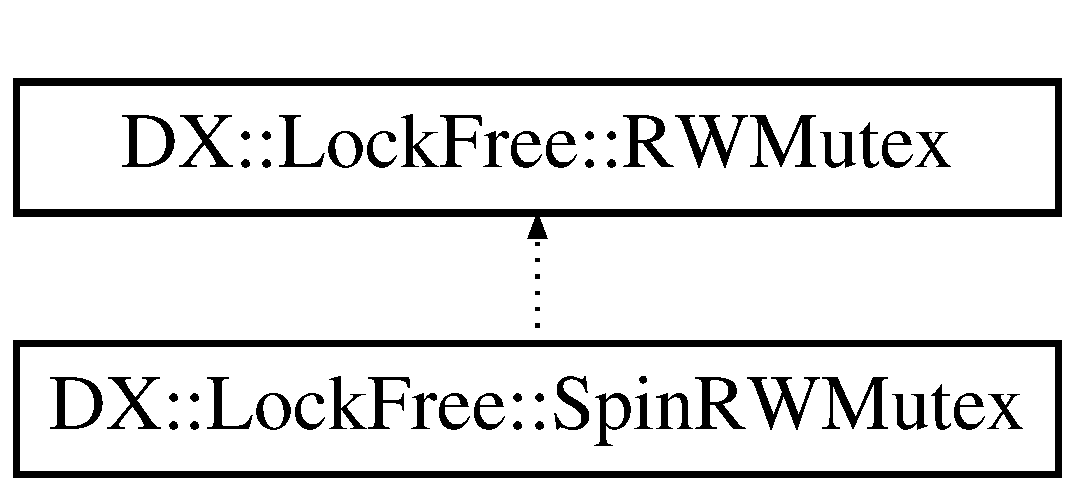
\includegraphics[height=2.000000cm]{class_d_x_1_1_lock_free_1_1_r_w_mutex}
\end{center}
\end{figure}
\subsection*{Public Member Functions}
\begin{DoxyCompactItemize}
\item 
virtual void \hyperlink{class_d_x_1_1_lock_free_1_1_r_w_mutex_a52009c1be555162b437e2c53eb3026c4}{lock\-Reader} () const =0
\item 
virtual void \hyperlink{class_d_x_1_1_lock_free_1_1_r_w_mutex_aaa10a03593e166b02c99455645b49800}{lock\-Writer} () const =0
\item 
virtual void \hyperlink{class_d_x_1_1_lock_free_1_1_r_w_mutex_a52ac4bfa7f6104ef271f468f2bb69eae}{unlock\-Reader} () const =0
\item 
virtual void \hyperlink{class_d_x_1_1_lock_free_1_1_r_w_mutex_af5d65dc65d6800b73d93b43cb7de559b}{unlock\-Writer} () const =0
\end{DoxyCompactItemize}


\subsection{Detailed Description}
\hyperlink{class_d_x_1_1_lock_free_1_1_r_w_mutex}{R\-W\-Mutex} is a general descriptor for a class of mutex-\/like objects that support multiple readers or a single writer. Unlike their \hyperlink{class_d_x_1_1_lock_free_1_1_mutex}{Mutex} counterparts, R\-W\-Mutexes have two different lock() and unlock() methods -\/ one set for writers and one set for readers. 

\subsection{Member Function Documentation}
\hypertarget{class_d_x_1_1_lock_free_1_1_r_w_mutex_a52009c1be555162b437e2c53eb3026c4}{\index{D\-X\-::\-Lock\-Free\-::\-R\-W\-Mutex@{D\-X\-::\-Lock\-Free\-::\-R\-W\-Mutex}!lock\-Reader@{lock\-Reader}}
\index{lock\-Reader@{lock\-Reader}!DX::LockFree::RWMutex@{D\-X\-::\-Lock\-Free\-::\-R\-W\-Mutex}}
\subsubsection[{lock\-Reader}]{\setlength{\rightskip}{0pt plus 5cm}virtual void D\-X\-::\-Lock\-Free\-::\-R\-W\-Mutex\-::lock\-Reader (
\begin{DoxyParamCaption}
{}
\end{DoxyParamCaption}
) const\hspace{0.3cm}{\ttfamily [pure virtual]}}}\label{class_d_x_1_1_lock_free_1_1_r_w_mutex_a52009c1be555162b437e2c53eb3026c4}
Locks this \hyperlink{class_d_x_1_1_lock_free_1_1_r_w_mutex}{R\-W\-Mutex} as a reader. Depending on the state of the object, this call may or may not block.

\begin{DoxyNote}{Note}
This call is gauranteed to not block if only readers have locks. Unspecified otherwise. 
\end{DoxyNote}


Implemented in \hyperlink{class_d_x_1_1_lock_free_1_1_spin_r_w_mutex_a71e9aef3a5e51ca1f74b765e3b123261}{D\-X\-::\-Lock\-Free\-::\-Spin\-R\-W\-Mutex}.

\hypertarget{class_d_x_1_1_lock_free_1_1_r_w_mutex_aaa10a03593e166b02c99455645b49800}{\index{D\-X\-::\-Lock\-Free\-::\-R\-W\-Mutex@{D\-X\-::\-Lock\-Free\-::\-R\-W\-Mutex}!lock\-Writer@{lock\-Writer}}
\index{lock\-Writer@{lock\-Writer}!DX::LockFree::RWMutex@{D\-X\-::\-Lock\-Free\-::\-R\-W\-Mutex}}
\subsubsection[{lock\-Writer}]{\setlength{\rightskip}{0pt plus 5cm}virtual void D\-X\-::\-Lock\-Free\-::\-R\-W\-Mutex\-::lock\-Writer (
\begin{DoxyParamCaption}
{}
\end{DoxyParamCaption}
) const\hspace{0.3cm}{\ttfamily [pure virtual]}}}\label{class_d_x_1_1_lock_free_1_1_r_w_mutex_aaa10a03593e166b02c99455645b49800}
Locks this \hyperlink{class_d_x_1_1_lock_free_1_1_r_w_mutex}{R\-W\-Mutex} as a writer. Depending on the state of the object, this call may or may not block.

\begin{DoxyNote}{Note}
This call is gauranteed not to block if there are no other readers or writers that have the \hyperlink{class_d_x_1_1_lock_free_1_1_r_w_mutex}{R\-W\-Mutex} locked. Unspecified otherwise. 
\end{DoxyNote}


Implemented in \hyperlink{class_d_x_1_1_lock_free_1_1_spin_r_w_mutex_a183780cdd01f30fef36febe8e7a7f9b7}{D\-X\-::\-Lock\-Free\-::\-Spin\-R\-W\-Mutex}.

\hypertarget{class_d_x_1_1_lock_free_1_1_r_w_mutex_a52ac4bfa7f6104ef271f468f2bb69eae}{\index{D\-X\-::\-Lock\-Free\-::\-R\-W\-Mutex@{D\-X\-::\-Lock\-Free\-::\-R\-W\-Mutex}!unlock\-Reader@{unlock\-Reader}}
\index{unlock\-Reader@{unlock\-Reader}!DX::LockFree::RWMutex@{D\-X\-::\-Lock\-Free\-::\-R\-W\-Mutex}}
\subsubsection[{unlock\-Reader}]{\setlength{\rightskip}{0pt plus 5cm}virtual void D\-X\-::\-Lock\-Free\-::\-R\-W\-Mutex\-::unlock\-Reader (
\begin{DoxyParamCaption}
{}
\end{DoxyParamCaption}
) const\hspace{0.3cm}{\ttfamily [pure virtual]}}}\label{class_d_x_1_1_lock_free_1_1_r_w_mutex_a52ac4bfa7f6104ef271f468f2bb69eae}
Releases a reader lock on the \hyperlink{class_d_x_1_1_lock_free_1_1_r_w_mutex}{R\-W\-Mutex}. This call does not block. \begin{DoxyNote}{Note}
Assumes that this call has been properly paired with a call to \hyperlink{class_d_x_1_1_lock_free_1_1_r_w_mutex_a52009c1be555162b437e2c53eb3026c4}{lock\-Reader()} 
\end{DoxyNote}


Implemented in \hyperlink{class_d_x_1_1_lock_free_1_1_spin_r_w_mutex_a64d2de6d900ba6eaeea1a0a76ac4ff5d}{D\-X\-::\-Lock\-Free\-::\-Spin\-R\-W\-Mutex}.

\hypertarget{class_d_x_1_1_lock_free_1_1_r_w_mutex_af5d65dc65d6800b73d93b43cb7de559b}{\index{D\-X\-::\-Lock\-Free\-::\-R\-W\-Mutex@{D\-X\-::\-Lock\-Free\-::\-R\-W\-Mutex}!unlock\-Writer@{unlock\-Writer}}
\index{unlock\-Writer@{unlock\-Writer}!DX::LockFree::RWMutex@{D\-X\-::\-Lock\-Free\-::\-R\-W\-Mutex}}
\subsubsection[{unlock\-Writer}]{\setlength{\rightskip}{0pt plus 5cm}virtual void D\-X\-::\-Lock\-Free\-::\-R\-W\-Mutex\-::unlock\-Writer (
\begin{DoxyParamCaption}
{}
\end{DoxyParamCaption}
) const\hspace{0.3cm}{\ttfamily [pure virtual]}}}\label{class_d_x_1_1_lock_free_1_1_r_w_mutex_af5d65dc65d6800b73d93b43cb7de559b}
Releases a writerer lock on the \hyperlink{class_d_x_1_1_lock_free_1_1_r_w_mutex}{R\-W\-Mutex}. This call does not block. \begin{DoxyNote}{Note}
Assumes that this call has been properly paired with a call to \hyperlink{class_d_x_1_1_lock_free_1_1_r_w_mutex_aaa10a03593e166b02c99455645b49800}{lock\-Writer()} 
\end{DoxyNote}


Implemented in \hyperlink{class_d_x_1_1_lock_free_1_1_spin_r_w_mutex_af20a514e5cc56ac5fbf6ab7759fafe1c}{D\-X\-::\-Lock\-Free\-::\-Spin\-R\-W\-Mutex}.



The documentation for this class was generated from the following files\-:\begin{DoxyCompactItemize}
\item 
Lock\-Free/\-Mutex/R\-W\-Mutex.\-h\item 
Lock\-Free/\-Mutex/R\-W\-Mutex.\-cpp\end{DoxyCompactItemize}

\hypertarget{classstd_1_1shared__ptr}{\section{std\-:\-:shared\-\_\-ptr$<$ T $>$ Class Template Reference}
\label{classstd_1_1shared__ptr}\index{std\-::shared\-\_\-ptr$<$ T $>$@{std\-::shared\-\_\-ptr$<$ T $>$}}
}


The documentation for this class was generated from the following file\-:\begin{DoxyCompactItemize}
\item 
Audio/\-Filters/Abstract\-Filter.\-h\end{DoxyCompactItemize}

\hypertarget{class_d_x_1_1_lock_free_1_1_spin_barrier}{\section{D\-X\-:\-:Lock\-Free\-:\-:Spin\-Barrier Class Reference}
\label{class_d_x_1_1_lock_free_1_1_spin_barrier}\index{D\-X\-::\-Lock\-Free\-::\-Spin\-Barrier@{D\-X\-::\-Lock\-Free\-::\-Spin\-Barrier}}
}


\hyperlink{class_d_x_1_1_lock_free_1_1_spin_barrier}{Spin\-Barrier} is designed for use to synchronize workflow between multiple threads. Calls to \hyperlink{class_d_x_1_1_lock_free_1_1_spin_barrier_a869688c05d8edae270a0e549c36c163d}{wait()} will block until some specified number of threads have called \hyperlink{class_d_x_1_1_lock_free_1_1_spin_barrier_a869688c05d8edae270a0e549c36c163d}{wait()}, after which all threads will unblock and continue execution.  




{\ttfamily \#include $<$Spin\-Barrier.\-h$>$}

Inheritance diagram for D\-X\-:\-:Lock\-Free\-:\-:Spin\-Barrier\-:\begin{figure}[H]
\begin{center}
\leavevmode
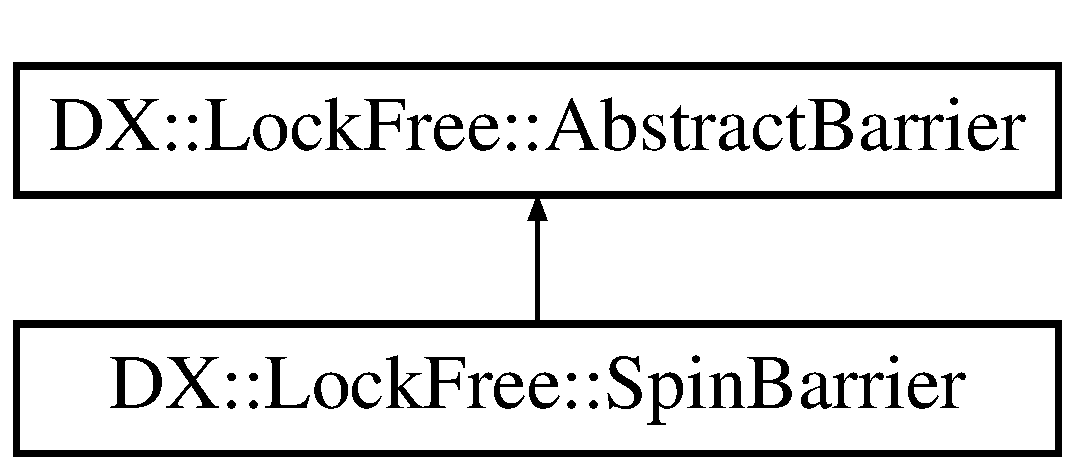
\includegraphics[height=2.000000cm]{class_d_x_1_1_lock_free_1_1_spin_barrier}
\end{center}
\end{figure}
\subsection*{Public Member Functions}
\begin{DoxyCompactItemize}
\item 
\hyperlink{class_d_x_1_1_lock_free_1_1_spin_barrier_acdde1ae097ee3f67636e3da90dae341d}{Spin\-Barrier} (size\-\_\-t num\-Threads=2)
\item 
\hyperlink{class_d_x_1_1_lock_free_1_1_spin_barrier_acbcdf2ddd0a3a682cca03b8950f48db3}{$\sim$\-Spin\-Barrier} ()
\item 
void \hyperlink{class_d_x_1_1_lock_free_1_1_spin_barrier_a869688c05d8edae270a0e549c36c163d}{wait} () const 
\item 
void \hyperlink{class_d_x_1_1_lock_free_1_1_spin_barrier_aea53e68d38677f716835dd5ad80279ba}{reset} ()
\end{DoxyCompactItemize}
\subsection*{Additional Inherited Members}


\subsection{Detailed Description}
\hyperlink{class_d_x_1_1_lock_free_1_1_spin_barrier}{Spin\-Barrier} is designed for use to synchronize workflow between multiple threads. Calls to \hyperlink{class_d_x_1_1_lock_free_1_1_spin_barrier_a869688c05d8edae270a0e549c36c163d}{wait()} will block until some specified number of threads have called \hyperlink{class_d_x_1_1_lock_free_1_1_spin_barrier_a869688c05d8edae270a0e549c36c163d}{wait()}, after which all threads will unblock and continue execution. 

\begin{DoxyNote}{Note}
\hyperlink{class_d_x_1_1_lock_free_1_1_spin_barrier}{Spin\-Barrier} is a form of a single-\/use barrier. For continued use, call \hyperlink{class_d_x_1_1_lock_free_1_1_spin_barrier_aea53e68d38677f716835dd5ad80279ba}{reset()} in a threadsafe fashion. 
\end{DoxyNote}


\subsection{Constructor \& Destructor Documentation}
\hypertarget{class_d_x_1_1_lock_free_1_1_spin_barrier_acdde1ae097ee3f67636e3da90dae341d}{\index{D\-X\-::\-Lock\-Free\-::\-Spin\-Barrier@{D\-X\-::\-Lock\-Free\-::\-Spin\-Barrier}!Spin\-Barrier@{Spin\-Barrier}}
\index{Spin\-Barrier@{Spin\-Barrier}!DX::LockFree::SpinBarrier@{D\-X\-::\-Lock\-Free\-::\-Spin\-Barrier}}
\subsubsection[{Spin\-Barrier}]{\setlength{\rightskip}{0pt plus 5cm}D\-X\-::\-Lock\-Free\-::\-Spin\-Barrier\-::\-Spin\-Barrier (
\begin{DoxyParamCaption}
\item[{size\-\_\-t}]{num\-Threads = {\ttfamily 2}}
\end{DoxyParamCaption}
)}}\label{class_d_x_1_1_lock_free_1_1_spin_barrier_acdde1ae097ee3f67636e3da90dae341d}
Constructs a \hyperlink{class_d_x_1_1_lock_free_1_1_spin_barrier}{Spin\-Barrier} that is set up to wait on some number of threads 
\begin{DoxyParams}[1]{Parameters}
\mbox{\tt in}  & {\em num\-Threads} & The number of threads that are expected to use this barrier \\
\hline
\end{DoxyParams}
\hypertarget{class_d_x_1_1_lock_free_1_1_spin_barrier_acbcdf2ddd0a3a682cca03b8950f48db3}{\index{D\-X\-::\-Lock\-Free\-::\-Spin\-Barrier@{D\-X\-::\-Lock\-Free\-::\-Spin\-Barrier}!$\sim$\-Spin\-Barrier@{$\sim$\-Spin\-Barrier}}
\index{$\sim$\-Spin\-Barrier@{$\sim$\-Spin\-Barrier}!DX::LockFree::SpinBarrier@{D\-X\-::\-Lock\-Free\-::\-Spin\-Barrier}}
\subsubsection[{$\sim$\-Spin\-Barrier}]{\setlength{\rightskip}{0pt plus 5cm}D\-X\-::\-Lock\-Free\-::\-Spin\-Barrier\-::$\sim$\-Spin\-Barrier (
\begin{DoxyParamCaption}
{}
\end{DoxyParamCaption}
)}}\label{class_d_x_1_1_lock_free_1_1_spin_barrier_acbcdf2ddd0a3a682cca03b8950f48db3}
Blocks the current thread of execution until all other \hyperlink{class_d_x_1_1_lock_free_1_1_spin_barrier_a869688c05d8edae270a0e549c36c163d}{wait()} calls have been made 

\subsection{Member Function Documentation}
\hypertarget{class_d_x_1_1_lock_free_1_1_spin_barrier_aea53e68d38677f716835dd5ad80279ba}{\index{D\-X\-::\-Lock\-Free\-::\-Spin\-Barrier@{D\-X\-::\-Lock\-Free\-::\-Spin\-Barrier}!reset@{reset}}
\index{reset@{reset}!DX::LockFree::SpinBarrier@{D\-X\-::\-Lock\-Free\-::\-Spin\-Barrier}}
\subsubsection[{reset}]{\setlength{\rightskip}{0pt plus 5cm}void D\-X\-::\-Lock\-Free\-::\-Spin\-Barrier\-::reset (
\begin{DoxyParamCaption}
{}
\end{DoxyParamCaption}
)}}\label{class_d_x_1_1_lock_free_1_1_spin_barrier_aea53e68d38677f716835dd5ad80279ba}
Resets the \hyperlink{class_d_x_1_1_lock_free_1_1_spin_barrier}{Spin\-Barrier} to its initial state, for continued usage.

\begin{DoxyNote}{Note}
\hyperlink{class_d_x_1_1_lock_free_1_1_spin_barrier_aea53e68d38677f716835dd5ad80279ba}{reset()} is N\-O\-T thread safe. 
\end{DoxyNote}
\hypertarget{class_d_x_1_1_lock_free_1_1_spin_barrier_a869688c05d8edae270a0e549c36c163d}{\index{D\-X\-::\-Lock\-Free\-::\-Spin\-Barrier@{D\-X\-::\-Lock\-Free\-::\-Spin\-Barrier}!wait@{wait}}
\index{wait@{wait}!DX::LockFree::SpinBarrier@{D\-X\-::\-Lock\-Free\-::\-Spin\-Barrier}}
\subsubsection[{wait}]{\setlength{\rightskip}{0pt plus 5cm}void D\-X\-::\-Lock\-Free\-::\-Spin\-Barrier\-::wait (
\begin{DoxyParamCaption}
{}
\end{DoxyParamCaption}
) const\hspace{0.3cm}{\ttfamily [virtual]}}}\label{class_d_x_1_1_lock_free_1_1_spin_barrier_a869688c05d8edae270a0e549c36c163d}
Blocks the current thread of execution until all other \hyperlink{class_d_x_1_1_lock_free_1_1_spin_barrier_a869688c05d8edae270a0e549c36c163d}{wait()} calls have beem made 

Implements \hyperlink{class_d_x_1_1_lock_free_1_1_abstract_barrier_a9040adf7507467e5a653bdaf2fbd17a6}{D\-X\-::\-Lock\-Free\-::\-Abstract\-Barrier}.



The documentation for this class was generated from the following files\-:\begin{DoxyCompactItemize}
\item 
Lock\-Free/\-Mutex/Spin\-Barrier.\-h\item 
Lock\-Free/\-Mutex/Spin\-Barrier.\-cpp\end{DoxyCompactItemize}

\hypertarget{class_d_x_1_1_lock_free_1_1_spin_lock}{\section{D\-X\-:\-:Lock\-Free\-:\-:Spin\-Lock Class Reference}
\label{class_d_x_1_1_lock_free_1_1_spin_lock}\index{D\-X\-::\-Lock\-Free\-::\-Spin\-Lock@{D\-X\-::\-Lock\-Free\-::\-Spin\-Lock}}
}


\hyperlink{class_d_x_1_1_lock_free_1_1_spin_lock}{Spin\-Lock} is a lock-\/guard style class that latches onto a mutex, locking it upon creation and unlocking it upon destruction.  




{\ttfamily \#include $<$Spin\-Mutex.\-h$>$}

\subsection*{Public Member Functions}
\begin{DoxyCompactItemize}
\item 
\hyperlink{class_d_x_1_1_lock_free_1_1_spin_lock_ad45dfee6c7aa94a6b6f195f1dc2f9e57}{Spin\-Lock} (const \hyperlink{class_d_x_1_1_lock_free_1_1_spin_mutex}{Spin\-Mutex} \&mutex)
\end{DoxyCompactItemize}


\subsection{Detailed Description}
\hyperlink{class_d_x_1_1_lock_free_1_1_spin_lock}{Spin\-Lock} is a lock-\/guard style class that latches onto a mutex, locking it upon creation and unlocking it upon destruction. 

Spin\-Locks are the preferred way of interacting with \hyperlink{class_d_x_1_1_lock_free_1_1_spin_mutex}{Spin\-Mutex}.

\begin{DoxyNote}{Note}
Spin\-Locks do not allow for recursive locking of a \hyperlink{class_d_x_1_1_lock_free_1_1_spin_mutex}{Spin\-Mutex}
\end{DoxyNote}
Here are two examples of using Spin\-Locks to protect critical sections of code\-: 
\begin{DoxyCode}
MyClass myClass;
SpinMutex myMutex;

\textcolor{keywordtype}{void} getMyClass()\textcolor{keyword}{ const}
\textcolor{keyword}{}\{
    \hyperlink{class_d_x_1_1_lock_free_1_1_spin_lock_ad45dfee6c7aa94a6b6f195f1dc2f9e57}{SpinLock} \_lock(myMutex);
    \textcolor{keywordflow}{return} myClass; \textcolor{comment}{// After the return, \_lock destroys itself, automatically unlocking myMutex}
\}
\end{DoxyCode}



\begin{DoxyCode}
MyClass myClass;
SpinMutex myMutex;

\textcolor{keywordtype}{void} doSomeThings(\textcolor{keyword}{const} MyClass& other)
\{
    \textcolor{comment}{// The below scope is thread-safe, the rest of the function isn't}
    \{
        \hyperlink{class_d_x_1_1_lock_free_1_1_spin_lock_ad45dfee6c7aa94a6b6f195f1dc2f9e57}{SpinLock} \_lock(myMutex);
        myClass = other;
    \}
    \textcolor{comment}{// Continue doing things here - the mutex is unlocked!}
\}
\end{DoxyCode}
 

\subsection{Constructor \& Destructor Documentation}
\hypertarget{class_d_x_1_1_lock_free_1_1_spin_lock_ad45dfee6c7aa94a6b6f195f1dc2f9e57}{\index{D\-X\-::\-Lock\-Free\-::\-Spin\-Lock@{D\-X\-::\-Lock\-Free\-::\-Spin\-Lock}!Spin\-Lock@{Spin\-Lock}}
\index{Spin\-Lock@{Spin\-Lock}!DX::LockFree::SpinLock@{D\-X\-::\-Lock\-Free\-::\-Spin\-Lock}}
\subsubsection[{Spin\-Lock}]{\setlength{\rightskip}{0pt plus 5cm}D\-X\-::\-Lock\-Free\-::\-Spin\-Lock\-::\-Spin\-Lock (
\begin{DoxyParamCaption}
\item[{const {\bf Spin\-Mutex} \&}]{mutex}
\end{DoxyParamCaption}
)}}\label{class_d_x_1_1_lock_free_1_1_spin_lock_ad45dfee6c7aa94a6b6f195f1dc2f9e57}

\begin{DoxyParams}[1]{Parameters}
\mbox{\tt in}  & {\em mutex} & The \hyperlink{class_d_x_1_1_lock_free_1_1_spin_mutex}{Spin\-Mutex} the lock will lock and guard \\
\hline
\end{DoxyParams}


The documentation for this class was generated from the following files\-:\begin{DoxyCompactItemize}
\item 
Lock\-Free/\-Mutex/Spin\-Mutex.\-h\item 
Lock\-Free/\-Mutex/Spin\-Mutex.\-cpp\end{DoxyCompactItemize}

\hypertarget{class_d_x_1_1_lock_free_1_1_spin_mutex}{\section{D\-X\-:\-:Lock\-Free\-:\-:Spin\-Mutex Class Reference}
\label{class_d_x_1_1_lock_free_1_1_spin_mutex}\index{D\-X\-::\-Lock\-Free\-::\-Spin\-Mutex@{D\-X\-::\-Lock\-Free\-::\-Spin\-Mutex}}
}


\hyperlink{class_d_x_1_1_lock_free_1_1_spin_mutex}{Spin\-Mutex} is a leightweight mutex class that makes use of C++11 atomics to spin out in active-\/\-C\-P\-U-\/land as opposed to the traditional method of yielding context. It's target use-\/case is for code regions that aren't too highly contended, or for contended regions that execute fairly fast.  




{\ttfamily \#include $<$Spin\-Mutex.\-h$>$}

Inheritance diagram for D\-X\-:\-:Lock\-Free\-:\-:Spin\-Mutex\-:\begin{figure}[H]
\begin{center}
\leavevmode
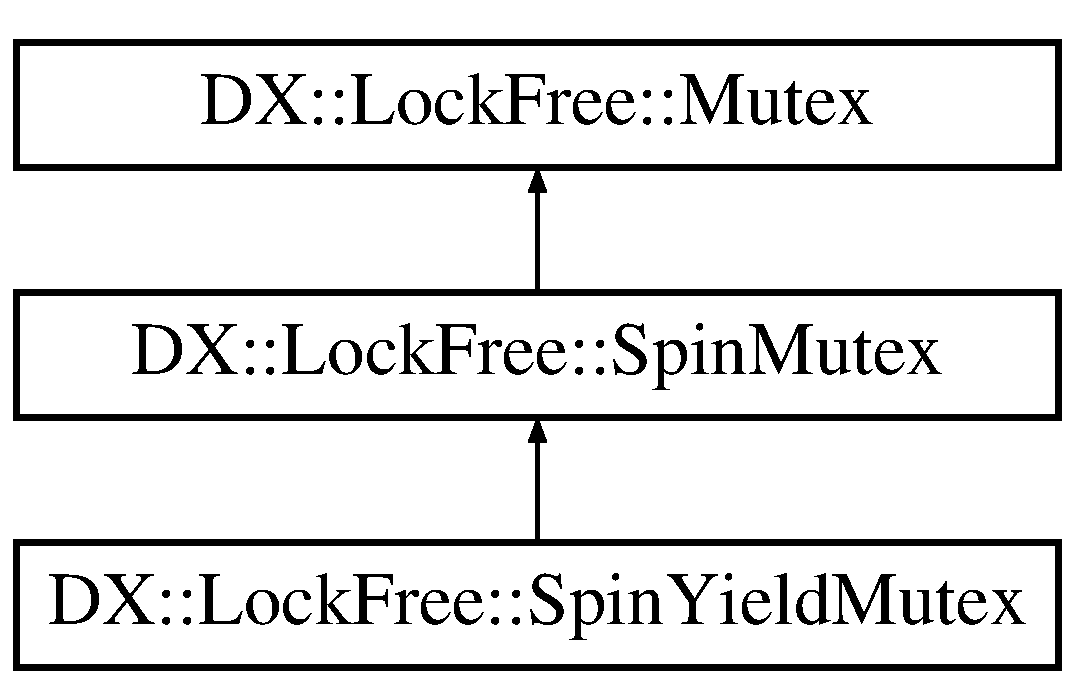
\includegraphics[height=3.000000cm]{class_d_x_1_1_lock_free_1_1_spin_mutex}
\end{center}
\end{figure}
\subsection*{Public Member Functions}
\begin{DoxyCompactItemize}
\item 
virtual void \hyperlink{class_d_x_1_1_lock_free_1_1_spin_mutex_aafeea5a756257e1297c65c58608959f0}{lock} () const 
\begin{DoxyCompactList}\small\item\em Locks the mutex. Further calls to lock will block until there is a call to \hyperlink{class_d_x_1_1_lock_free_1_1_spin_mutex_a570be8426468711010b98e5c9a9c1fa1}{unlock()}. \end{DoxyCompactList}\item 
virtual bool \hyperlink{class_d_x_1_1_lock_free_1_1_spin_mutex_aeb3f7133cb914cafd0f7f484e6a08584}{try\-Lock} () const 
\begin{DoxyCompactList}\small\item\em Attempts to lock the mutex. \hyperlink{class_d_x_1_1_lock_free_1_1_spin_mutex_aeb3f7133cb914cafd0f7f484e6a08584}{try\-Lock()} is non-\/blocking, meaning that regardless of the state of the mutex when \hyperlink{class_d_x_1_1_lock_free_1_1_spin_mutex_aeb3f7133cb914cafd0f7f484e6a08584}{try\-Lock()} is called, execution will continue. \end{DoxyCompactList}\item 
\hypertarget{class_d_x_1_1_lock_free_1_1_spin_mutex_a570be8426468711010b98e5c9a9c1fa1}{virtual void \hyperlink{class_d_x_1_1_lock_free_1_1_spin_mutex_a570be8426468711010b98e5c9a9c1fa1}{unlock} () const }\label{class_d_x_1_1_lock_free_1_1_spin_mutex_a570be8426468711010b98e5c9a9c1fa1}

\begin{DoxyCompactList}\small\item\em Unlocks the mutex. This call is non-\/blocking, because having it otherwise doesn't make any sense. \end{DoxyCompactList}\end{DoxyCompactItemize}
\subsection*{Protected Attributes}
\begin{DoxyCompactItemize}
\item 
\hypertarget{class_d_x_1_1_lock_free_1_1_spin_mutex_a88931806ac093b52121aa5a6cf19a496}{volatile char {\bfseries pad\-\_\-0} \mbox{[}C\-A\-C\-H\-E\-\_\-\-L\-I\-N\-E\-\_\-\-S\-I\-Z\-E\mbox{]}}\label{class_d_x_1_1_lock_free_1_1_spin_mutex_a88931806ac093b52121aa5a6cf19a496}

\item 
\hypertarget{class_d_x_1_1_lock_free_1_1_spin_mutex_a69aa18fcecdee6f6396f5b886b1ca81a}{std\-::atomic$<$ bool $>$ {\bfseries m\-\_\-lock}}\label{class_d_x_1_1_lock_free_1_1_spin_mutex_a69aa18fcecdee6f6396f5b886b1ca81a}

\item 
\hypertarget{class_d_x_1_1_lock_free_1_1_spin_mutex_a6e03110e19e13a55d6e2c270285adb0d}{volatile char {\bfseries pad\-\_\-1} \mbox{[}C\-A\-C\-H\-E\-\_\-\-L\-I\-N\-E\-\_\-\-S\-I\-Z\-E-\/(sizeof(std\-::atomic$<$ bool $>$)\%C\-A\-C\-H\-E\-\_\-\-L\-I\-N\-E\-\_\-\-S\-I\-Z\-E)\mbox{]}}\label{class_d_x_1_1_lock_free_1_1_spin_mutex_a6e03110e19e13a55d6e2c270285adb0d}

\end{DoxyCompactItemize}


\subsection{Detailed Description}
\hyperlink{class_d_x_1_1_lock_free_1_1_spin_mutex}{Spin\-Mutex} is a leightweight mutex class that makes use of C++11 atomics to spin out in active-\/\-C\-P\-U-\/land as opposed to the traditional method of yielding context. It's target use-\/case is for code regions that aren't too highly contended, or for contended regions that execute fairly fast. 

\begin{DoxyNote}{Note}
\hyperlink{class_d_x_1_1_lock_free_1_1_spin_mutex}{Spin\-Mutex} is not a recursive mutex
\end{DoxyNote}
Sample of a \hyperlink{class_d_x_1_1_lock_free_1_1_spin_mutex}{Spin\-Mutex} protecting an int\-: 
\begin{DoxyCode}
\textcolor{keyword}{mutable} SpinMutex myMutex;
\textcolor{keywordtype}{int} myProtectedValue; 

\textcolor{keywordtype}{void} setMyValue(\textcolor{keywordtype}{int} newValue)
\{
    myMutex.lock();
    myProtectedValue = newValue;
    myMutex.unlock();
\}

\textcolor{keywordtype}{int} getMyValue()\textcolor{keyword}{ const}
\textcolor{keyword}{}\{
    \textcolor{keywordtype}{int} ret;
    myMutex.lock();
    ret = myProtectedValue;
    myMutex.unlock();

    \textcolor{keywordflow}{return} ret;
\}
\end{DoxyCode}


Please note that the above example could also be accomplished by making the type of my\-Protected\-Value std\-::atomic$<$int$>$, but the usage still stands. 

\subsection{Member Function Documentation}
\hypertarget{class_d_x_1_1_lock_free_1_1_spin_mutex_aafeea5a756257e1297c65c58608959f0}{\index{D\-X\-::\-Lock\-Free\-::\-Spin\-Mutex@{D\-X\-::\-Lock\-Free\-::\-Spin\-Mutex}!lock@{lock}}
\index{lock@{lock}!DX::LockFree::SpinMutex@{D\-X\-::\-Lock\-Free\-::\-Spin\-Mutex}}
\subsubsection[{lock}]{\setlength{\rightskip}{0pt plus 5cm}void D\-X\-::\-Lock\-Free\-::\-Spin\-Mutex\-::lock (
\begin{DoxyParamCaption}
{}
\end{DoxyParamCaption}
) const\hspace{0.3cm}{\ttfamily [virtual]}}}\label{class_d_x_1_1_lock_free_1_1_spin_mutex_aafeea5a756257e1297c65c58608959f0}


Locks the mutex. Further calls to lock will block until there is a call to \hyperlink{class_d_x_1_1_lock_free_1_1_spin_mutex_a570be8426468711010b98e5c9a9c1fa1}{unlock()}. 

\begin{DoxyNote}{Note}
\hyperlink{class_d_x_1_1_lock_free_1_1_spin_mutex_aafeea5a756257e1297c65c58608959f0}{lock()} is not recursive. 

\hyperlink{class_d_x_1_1_lock_free_1_1_spin_mutex_aafeea5a756257e1297c65c58608959f0}{lock()} is blocking. 
\end{DoxyNote}


Implements \hyperlink{class_d_x_1_1_lock_free_1_1_mutex}{D\-X\-::\-Lock\-Free\-::\-Mutex}.



Reimplemented in \hyperlink{class_d_x_1_1_lock_free_1_1_spin_yield_mutex_a4c505e87ee87dbaff9f872a0009fa942}{D\-X\-::\-Lock\-Free\-::\-Spin\-Yield\-Mutex}.

\hypertarget{class_d_x_1_1_lock_free_1_1_spin_mutex_aeb3f7133cb914cafd0f7f484e6a08584}{\index{D\-X\-::\-Lock\-Free\-::\-Spin\-Mutex@{D\-X\-::\-Lock\-Free\-::\-Spin\-Mutex}!try\-Lock@{try\-Lock}}
\index{try\-Lock@{try\-Lock}!DX::LockFree::SpinMutex@{D\-X\-::\-Lock\-Free\-::\-Spin\-Mutex}}
\subsubsection[{try\-Lock}]{\setlength{\rightskip}{0pt plus 5cm}bool D\-X\-::\-Lock\-Free\-::\-Spin\-Mutex\-::try\-Lock (
\begin{DoxyParamCaption}
{}
\end{DoxyParamCaption}
) const\hspace{0.3cm}{\ttfamily [virtual]}}}\label{class_d_x_1_1_lock_free_1_1_spin_mutex_aeb3f7133cb914cafd0f7f484e6a08584}


Attempts to lock the mutex. \hyperlink{class_d_x_1_1_lock_free_1_1_spin_mutex_aeb3f7133cb914cafd0f7f484e6a08584}{try\-Lock()} is non-\/blocking, meaning that regardless of the state of the mutex when \hyperlink{class_d_x_1_1_lock_free_1_1_spin_mutex_aeb3f7133cb914cafd0f7f484e6a08584}{try\-Lock()} is called, execution will continue. 

\begin{DoxyNote}{Note}
\hyperlink{class_d_x_1_1_lock_free_1_1_spin_mutex_aeb3f7133cb914cafd0f7f484e6a08584}{try\-Lock()} is not recursive. 

\hyperlink{class_d_x_1_1_lock_free_1_1_spin_mutex_aeb3f7133cb914cafd0f7f484e6a08584}{try\-Lock()} is non-\/blocking. 
\end{DoxyNote}


Reimplemented in \hyperlink{class_d_x_1_1_lock_free_1_1_spin_yield_mutex_a0d8fc55d539af89d8d8e04a61bb5e887}{D\-X\-::\-Lock\-Free\-::\-Spin\-Yield\-Mutex}.



The documentation for this class was generated from the following files\-:\begin{DoxyCompactItemize}
\item 
Lock\-Free/\-Mutex/Spin\-Mutex.\-h\item 
Lock\-Free/\-Mutex/Spin\-Mutex.\-cpp\end{DoxyCompactItemize}

\hypertarget{class_d_x_1_1_lock_free_1_1_spin_r_w_lock}{\section{D\-X\-:\-:Lock\-Free\-:\-:Spin\-R\-W\-Lock Class Reference}
\label{class_d_x_1_1_lock_free_1_1_spin_r_w_lock}\index{D\-X\-::\-Lock\-Free\-::\-Spin\-R\-W\-Lock@{D\-X\-::\-Lock\-Free\-::\-Spin\-R\-W\-Lock}}
}


\hyperlink{class_d_x_1_1_lock_free_1_1_spin_r_w_lock}{Spin\-R\-W\-Lock} is the preferred way of interacting with a \hyperlink{class_d_x_1_1_lock_free_1_1_spin_r_w_mutex}{Spin\-R\-W\-Mutex}. \hyperlink{class_d_x_1_1_lock_free_1_1_spin_r_w_lock}{Spin\-R\-W\-Lock} is a lock-\/guard style class, locking the \hyperlink{class_d_x_1_1_lock_free_1_1_spin_r_w_mutex}{Spin\-R\-W\-Mutex} upon construction and releasing the lock upon destruction. \hyperlink{class_d_x_1_1_lock_free_1_1_spin_r_w_mutex}{Spin\-R\-W\-Mutex} remembers whether it is a reader or writer lock, and releases the same kind of lock that it was constructed with.  




{\ttfamily \#include $<$Spin\-R\-W\-Mutex.\-h$>$}

\subsection*{Public Member Functions}
\begin{DoxyCompactItemize}
\item 
\hyperlink{class_d_x_1_1_lock_free_1_1_spin_r_w_lock_a079aadf792b936cee1e94e9f3870e1ba}{Spin\-R\-W\-Lock} (const \hyperlink{class_d_x_1_1_lock_free_1_1_spin_r_w_mutex}{Spin\-R\-W\-Mutex} \&mutex, bool is\-Writer)
\end{DoxyCompactItemize}


\subsection{Detailed Description}
\hyperlink{class_d_x_1_1_lock_free_1_1_spin_r_w_lock}{Spin\-R\-W\-Lock} is the preferred way of interacting with a \hyperlink{class_d_x_1_1_lock_free_1_1_spin_r_w_mutex}{Spin\-R\-W\-Mutex}. \hyperlink{class_d_x_1_1_lock_free_1_1_spin_r_w_lock}{Spin\-R\-W\-Lock} is a lock-\/guard style class, locking the \hyperlink{class_d_x_1_1_lock_free_1_1_spin_r_w_mutex}{Spin\-R\-W\-Mutex} upon construction and releasing the lock upon destruction. \hyperlink{class_d_x_1_1_lock_free_1_1_spin_r_w_mutex}{Spin\-R\-W\-Mutex} remembers whether it is a reader or writer lock, and releases the same kind of lock that it was constructed with. 

The big advantage of using Spin\-R\-W\-Locks over \hyperlink{class_d_x_1_1_lock_free_1_1_spin_r_w_mutex}{Spin\-R\-W\-Mutex} is the automatic unlock on destruction\-: unlike the examples provided above, no copies have to be made on a get() call

\begin{DoxyNote}{Note}
Spin\-R\-W\-Locks do not allow for recursive writer-\/locks of a single \hyperlink{class_d_x_1_1_lock_free_1_1_spin_r_w_mutex}{Spin\-R\-W\-Mutex}
\end{DoxyNote}

\begin{DoxyCode}
MyClass myClass;
\textcolor{keyword}{mutable} SpinRWMutex myRWMutex;

MyClass getMyClass()\textcolor{keyword}{ const}
\textcolor{keyword}{}\{
    \hyperlink{class_d_x_1_1_lock_free_1_1_spin_r_w_lock_a079aadf792b936cee1e94e9f3870e1ba}{SpinRWLock} \_lock(myRWMutex, \textcolor{keyword}{false});
    \textcolor{keywordflow}{return} myClass; \textcolor{comment}{// No copies or thread-local storage necessary}
\}

\textcolor{keywordtype}{void} setMyClass(\textcolor{keyword}{const} MyClass& other)
\{
    \hyperlink{class_d_x_1_1_lock_free_1_1_spin_r_w_lock_a079aadf792b936cee1e94e9f3870e1ba}{SpinRWLock} \_lock(myRWMutex, \textcolor{keyword}{true});
    myClass = other;
\}
\end{DoxyCode}
 

\subsection{Constructor \& Destructor Documentation}
\hypertarget{class_d_x_1_1_lock_free_1_1_spin_r_w_lock_a079aadf792b936cee1e94e9f3870e1ba}{\index{D\-X\-::\-Lock\-Free\-::\-Spin\-R\-W\-Lock@{D\-X\-::\-Lock\-Free\-::\-Spin\-R\-W\-Lock}!Spin\-R\-W\-Lock@{Spin\-R\-W\-Lock}}
\index{Spin\-R\-W\-Lock@{Spin\-R\-W\-Lock}!DX::LockFree::SpinRWLock@{D\-X\-::\-Lock\-Free\-::\-Spin\-R\-W\-Lock}}
\subsubsection[{Spin\-R\-W\-Lock}]{\setlength{\rightskip}{0pt plus 5cm}D\-X\-::\-Lock\-Free\-::\-Spin\-R\-W\-Lock\-::\-Spin\-R\-W\-Lock (
\begin{DoxyParamCaption}
\item[{const {\bf Spin\-R\-W\-Mutex} \&}]{mutex, }
\item[{bool}]{is\-Writer}
\end{DoxyParamCaption}
)}}\label{class_d_x_1_1_lock_free_1_1_spin_r_w_lock_a079aadf792b936cee1e94e9f3870e1ba}

\begin{DoxyParams}[1]{Parameters}
\mbox{\tt in}  & {\em mutex} & The \hyperlink{class_d_x_1_1_lock_free_1_1_spin_r_w_mutex}{Spin\-R\-W\-Mutex} that the lock should be locking/unlocking \\
\hline
\mbox{\tt in}  & {\em is\-Writer} & True indicates a writer lock, False indicates a reader lock \\
\hline
\end{DoxyParams}


The documentation for this class was generated from the following files\-:\begin{DoxyCompactItemize}
\item 
Lock\-Free/\-Mutex/Spin\-R\-W\-Mutex.\-h\item 
Lock\-Free/\-Mutex/Spin\-R\-W\-Mutex.\-cpp\end{DoxyCompactItemize}

\hypertarget{class_d_x_1_1_lock_free_1_1_spin_r_w_mutex}{\section{D\-X\-:\-:Lock\-Free\-:\-:Spin\-R\-W\-Mutex Class Reference}
\label{class_d_x_1_1_lock_free_1_1_spin_r_w_mutex}\index{D\-X\-::\-Lock\-Free\-::\-Spin\-R\-W\-Mutex@{D\-X\-::\-Lock\-Free\-::\-Spin\-R\-W\-Mutex}}
}


\hyperlink{class_d_x_1_1_lock_free_1_1_spin_r_w_mutex}{Spin\-R\-W\-Mutex} is a leightweight mutex that supports multiple readers (const-\/only access) and a single writer. Supports readers up to the maximum value of size\-\_\-t for your system.  




{\ttfamily \#include $<$Spin\-R\-W\-Mutex.\-h$>$}

Inheritance diagram for D\-X\-:\-:Lock\-Free\-:\-:Spin\-R\-W\-Mutex\-:\begin{figure}[H]
\begin{center}
\leavevmode
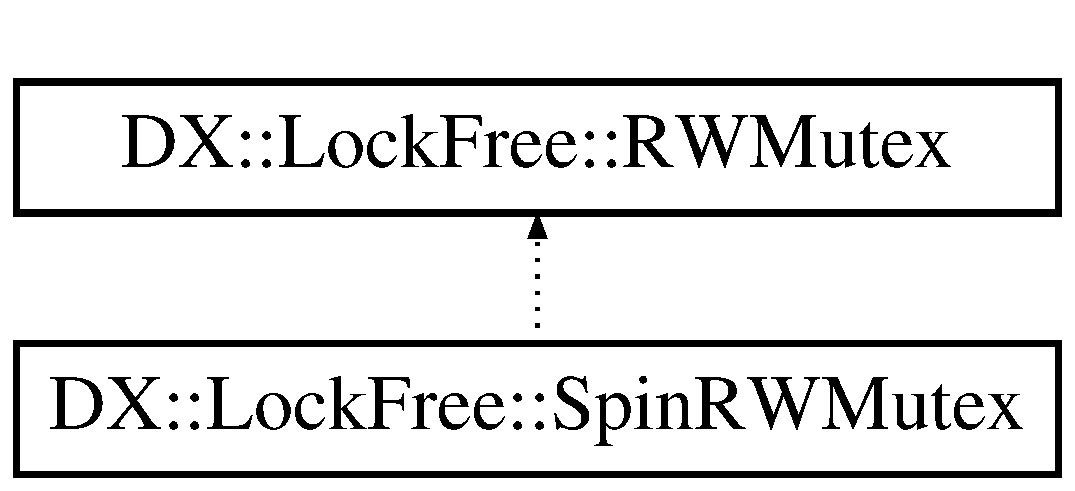
\includegraphics[height=2.000000cm]{class_d_x_1_1_lock_free_1_1_spin_r_w_mutex}
\end{center}
\end{figure}
\subsection*{Public Member Functions}
\begin{DoxyCompactItemize}
\item 
void \hyperlink{class_d_x_1_1_lock_free_1_1_spin_r_w_mutex_a71e9aef3a5e51ca1f74b765e3b123261}{lock\-Reader} () const 
\item 
void \hyperlink{class_d_x_1_1_lock_free_1_1_spin_r_w_mutex_a183780cdd01f30fef36febe8e7a7f9b7}{lock\-Writer} () const 
\item 
void \hyperlink{class_d_x_1_1_lock_free_1_1_spin_r_w_mutex_a64d2de6d900ba6eaeea1a0a76ac4ff5d}{unlock\-Reader} () const 
\item 
void \hyperlink{class_d_x_1_1_lock_free_1_1_spin_r_w_mutex_af20a514e5cc56ac5fbf6ab7759fafe1c}{unlock\-Writer} () const 
\end{DoxyCompactItemize}


\subsection{Detailed Description}
\hyperlink{class_d_x_1_1_lock_free_1_1_spin_r_w_mutex}{Spin\-R\-W\-Mutex} is a leightweight mutex that supports multiple readers (const-\/only access) and a single writer. Supports readers up to the maximum value of size\-\_\-t for your system. 

Calls to lock() from readers will block if a writer holds the lock. Calls to lock() from writers will block if there are any readers or writers holding onto the lock.

\begin{DoxyNote}{Note}
\hyperlink{class_d_x_1_1_lock_free_1_1_spin_r_w_mutex}{Spin\-R\-W\-Mutex} is favored towards writers attempting to get the lock

\hyperlink{class_d_x_1_1_lock_free_1_1_spin_r_w_mutex}{Spin\-R\-W\-Mutex} is easiest to use with \hyperlink{class_d_x_1_1_lock_free_1_1_spin_r_w_lock}{Spin\-R\-W\-Lock}. \hyperlink{class_d_x_1_1_lock_free_1_1_spin_r_w_lock}{Spin\-R\-W\-Lock} lets you \char`\"{}set-\/it-\/and-\/forget-\/it\char`\"{} in regards to remembering if you're a reader/writer.

\hyperlink{class_d_x_1_1_lock_free_1_1_spin_r_w_mutex}{Spin\-R\-W\-Mutex} does {\itshape N\-O\-T} check to ensure that calls to lock/unlock are called with the same boolean. It does handle these cases (crash-\/wise), but calling lock(true) and unlock(false) from the same thread does not unlock the writer lock.
\end{DoxyNote}

\begin{DoxyCode}
\textcolor{keyword}{mutable} SpinRWMutex myRWMutex;
MyClass myClass;

\textcolor{keywordtype}{void} setMyClass(\textcolor{keyword}{const} MyClass& other)
\{
    myRWMutex.lock(\textcolor{keyword}{true}); \textcolor{comment}{// true indicates a writer}
    myClass = other;
    myRWMutex.unlock(\textcolor{keyword}{true}); \textcolor{comment}{// unlock my writer reference            }
\}

MyClass getMyClass()\textcolor{keyword}{ const}
\textcolor{keyword}{}\{
    \textcolor{comment}{// static , thread-local object so it isn't constructed every function call, only copied}
    \textcolor{keyword}{static} thread\_local MyClass ret;
    myRWMutex.lock(\textcolor{keyword}{false}); \textcolor{comment}{// false indicates reader}
    ret = myClass;
    myRwMutex.unlock(\textcolor{keyword}{false}); \textcolor{comment}{// unlock my reader reference}
    \textcolor{keywordflow}{return} ret;
\}
\end{DoxyCode}
 

\subsection{Member Function Documentation}
\hypertarget{class_d_x_1_1_lock_free_1_1_spin_r_w_mutex_a71e9aef3a5e51ca1f74b765e3b123261}{\index{D\-X\-::\-Lock\-Free\-::\-Spin\-R\-W\-Mutex@{D\-X\-::\-Lock\-Free\-::\-Spin\-R\-W\-Mutex}!lock\-Reader@{lock\-Reader}}
\index{lock\-Reader@{lock\-Reader}!DX::LockFree::SpinRWMutex@{D\-X\-::\-Lock\-Free\-::\-Spin\-R\-W\-Mutex}}
\subsubsection[{lock\-Reader}]{\setlength{\rightskip}{0pt plus 5cm}void D\-X\-::\-Lock\-Free\-::\-Spin\-R\-W\-Mutex\-::lock\-Reader (
\begin{DoxyParamCaption}
{}
\end{DoxyParamCaption}
) const\hspace{0.3cm}{\ttfamily [virtual]}}}\label{class_d_x_1_1_lock_free_1_1_spin_r_w_mutex_a71e9aef3a5e51ca1f74b765e3b123261}
Locks this \hyperlink{class_d_x_1_1_lock_free_1_1_spin_r_w_mutex}{Spin\-R\-W\-Mutex} as a reader. Depending on the state of the object, this call may or may not block.

\begin{DoxyNote}{Note}
This call gauantees to not block if only readers have locks. Unspecified otherwise. 
\end{DoxyNote}


Implements \hyperlink{class_d_x_1_1_lock_free_1_1_r_w_mutex_a52009c1be555162b437e2c53eb3026c4}{D\-X\-::\-Lock\-Free\-::\-R\-W\-Mutex}.

\hypertarget{class_d_x_1_1_lock_free_1_1_spin_r_w_mutex_a183780cdd01f30fef36febe8e7a7f9b7}{\index{D\-X\-::\-Lock\-Free\-::\-Spin\-R\-W\-Mutex@{D\-X\-::\-Lock\-Free\-::\-Spin\-R\-W\-Mutex}!lock\-Writer@{lock\-Writer}}
\index{lock\-Writer@{lock\-Writer}!DX::LockFree::SpinRWMutex@{D\-X\-::\-Lock\-Free\-::\-Spin\-R\-W\-Mutex}}
\subsubsection[{lock\-Writer}]{\setlength{\rightskip}{0pt plus 5cm}void D\-X\-::\-Lock\-Free\-::\-Spin\-R\-W\-Mutex\-::lock\-Writer (
\begin{DoxyParamCaption}
{}
\end{DoxyParamCaption}
) const\hspace{0.3cm}{\ttfamily [virtual]}}}\label{class_d_x_1_1_lock_free_1_1_spin_r_w_mutex_a183780cdd01f30fef36febe8e7a7f9b7}
Locks this \hyperlink{class_d_x_1_1_lock_free_1_1_spin_r_w_mutex}{Spin\-R\-W\-Mutex} as a writer. Depending on the state of the object, this call may or may not block.

\begin{DoxyNote}{Note}
This call gauantees to not block if there are no other readers or writers currently have locks. Unspecified otherwsie. 
\end{DoxyNote}


Implements \hyperlink{class_d_x_1_1_lock_free_1_1_r_w_mutex_aaa10a03593e166b02c99455645b49800}{D\-X\-::\-Lock\-Free\-::\-R\-W\-Mutex}.

\hypertarget{class_d_x_1_1_lock_free_1_1_spin_r_w_mutex_a64d2de6d900ba6eaeea1a0a76ac4ff5d}{\index{D\-X\-::\-Lock\-Free\-::\-Spin\-R\-W\-Mutex@{D\-X\-::\-Lock\-Free\-::\-Spin\-R\-W\-Mutex}!unlock\-Reader@{unlock\-Reader}}
\index{unlock\-Reader@{unlock\-Reader}!DX::LockFree::SpinRWMutex@{D\-X\-::\-Lock\-Free\-::\-Spin\-R\-W\-Mutex}}
\subsubsection[{unlock\-Reader}]{\setlength{\rightskip}{0pt plus 5cm}void D\-X\-::\-Lock\-Free\-::\-Spin\-R\-W\-Mutex\-::unlock\-Reader (
\begin{DoxyParamCaption}
{}
\end{DoxyParamCaption}
) const\hspace{0.3cm}{\ttfamily [virtual]}}}\label{class_d_x_1_1_lock_free_1_1_spin_r_w_mutex_a64d2de6d900ba6eaeea1a0a76ac4ff5d}
Releases a reader lock on the \hyperlink{class_d_x_1_1_lock_free_1_1_spin_r_w_mutex}{Spin\-R\-W\-Mutex}. This call does not block. \begin{DoxyNote}{Note}
Assumes that this call has been properly paired with a call to \hyperlink{class_d_x_1_1_lock_free_1_1_spin_r_w_mutex_a71e9aef3a5e51ca1f74b765e3b123261}{lock\-Reader()} 
\end{DoxyNote}


Implements \hyperlink{class_d_x_1_1_lock_free_1_1_r_w_mutex_a52ac4bfa7f6104ef271f468f2bb69eae}{D\-X\-::\-Lock\-Free\-::\-R\-W\-Mutex}.

\hypertarget{class_d_x_1_1_lock_free_1_1_spin_r_w_mutex_af20a514e5cc56ac5fbf6ab7759fafe1c}{\index{D\-X\-::\-Lock\-Free\-::\-Spin\-R\-W\-Mutex@{D\-X\-::\-Lock\-Free\-::\-Spin\-R\-W\-Mutex}!unlock\-Writer@{unlock\-Writer}}
\index{unlock\-Writer@{unlock\-Writer}!DX::LockFree::SpinRWMutex@{D\-X\-::\-Lock\-Free\-::\-Spin\-R\-W\-Mutex}}
\subsubsection[{unlock\-Writer}]{\setlength{\rightskip}{0pt plus 5cm}void D\-X\-::\-Lock\-Free\-::\-Spin\-R\-W\-Mutex\-::unlock\-Writer (
\begin{DoxyParamCaption}
{}
\end{DoxyParamCaption}
) const\hspace{0.3cm}{\ttfamily [virtual]}}}\label{class_d_x_1_1_lock_free_1_1_spin_r_w_mutex_af20a514e5cc56ac5fbf6ab7759fafe1c}
Releases a writer lock on the \hyperlink{class_d_x_1_1_lock_free_1_1_spin_r_w_mutex}{Spin\-R\-W\-Mutex}. This call does not block. \begin{DoxyNote}{Note}
Assumes that this call has been properly paired with a call to \hyperlink{class_d_x_1_1_lock_free_1_1_spin_r_w_mutex_a183780cdd01f30fef36febe8e7a7f9b7}{lock\-Writer()} 
\end{DoxyNote}


Implements \hyperlink{class_d_x_1_1_lock_free_1_1_r_w_mutex_af5d65dc65d6800b73d93b43cb7de559b}{D\-X\-::\-Lock\-Free\-::\-R\-W\-Mutex}.



The documentation for this class was generated from the following files\-:\begin{DoxyCompactItemize}
\item 
Lock\-Free/\-Mutex/Spin\-R\-W\-Mutex.\-h\item 
Lock\-Free/\-Mutex/Spin\-R\-W\-Mutex.\-cpp\end{DoxyCompactItemize}

\hypertarget{class_d_x_1_1_lock_free_1_1_spin_yield_mutex}{\section{D\-X\-:\-:Lock\-Free\-:\-:Spin\-Yield\-Mutex Class Reference}
\label{class_d_x_1_1_lock_free_1_1_spin_yield_mutex}\index{D\-X\-::\-Lock\-Free\-::\-Spin\-Yield\-Mutex@{D\-X\-::\-Lock\-Free\-::\-Spin\-Yield\-Mutex}}
}
Inheritance diagram for D\-X\-:\-:Lock\-Free\-:\-:Spin\-Yield\-Mutex\-:\begin{figure}[H]
\begin{center}
\leavevmode
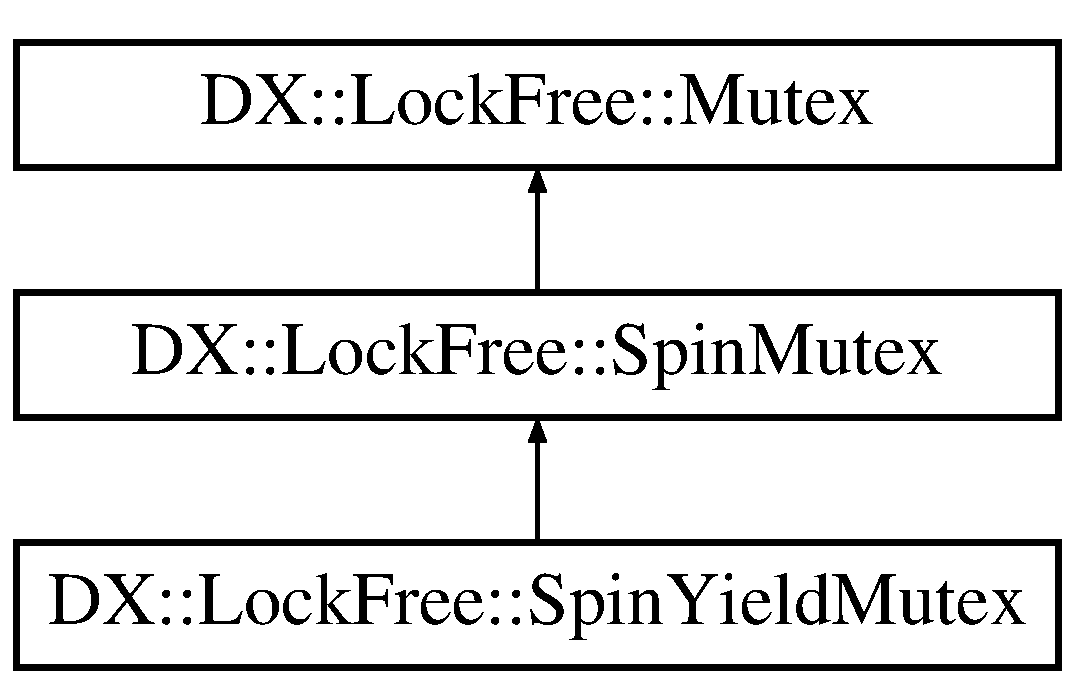
\includegraphics[height=3.000000cm]{class_d_x_1_1_lock_free_1_1_spin_yield_mutex}
\end{center}
\end{figure}
\subsection*{Public Member Functions}
\begin{DoxyCompactItemize}
\item 
\hyperlink{class_d_x_1_1_lock_free_1_1_spin_yield_mutex_a3c0996c0b9aab82e247df61a3a9dd38d}{Spin\-Yield\-Mutex} (const size\-\_\-t max\-Yield\-Ticks=D\-E\-F\-A\-U\-L\-T\-\_\-\-Y\-I\-E\-L\-D\-\_\-\-T\-I\-C\-K\-S)
\item 
\hyperlink{class_d_x_1_1_lock_free_1_1_spin_yield_mutex_a12abee65fbb86f2d4e5caf136941be0e}{$\sim$\-Spin\-Yield\-Mutex} ()
\item 
void \hyperlink{class_d_x_1_1_lock_free_1_1_spin_yield_mutex_a4c505e87ee87dbaff9f872a0009fa942}{lock} () const 
\item 
bool \hyperlink{class_d_x_1_1_lock_free_1_1_spin_yield_mutex_a0d8fc55d539af89d8d8e04a61bb5e887}{try\-Lock} () const 
\item 
\hypertarget{class_d_x_1_1_lock_free_1_1_spin_yield_mutex_ad428d031840d4a7679ea101c05095b7c}{void \hyperlink{class_d_x_1_1_lock_free_1_1_spin_yield_mutex_ad428d031840d4a7679ea101c05095b7c}{unlock} () const }\label{class_d_x_1_1_lock_free_1_1_spin_yield_mutex_ad428d031840d4a7679ea101c05095b7c}

\begin{DoxyCompactList}\small\item\em Unlocks the mutex. This call is non-\/blocking, because having it otherwise doesn't make any sense. \end{DoxyCompactList}\end{DoxyCompactItemize}
\subsection*{Additional Inherited Members}


\subsection{Constructor \& Destructor Documentation}
\hypertarget{class_d_x_1_1_lock_free_1_1_spin_yield_mutex_a3c0996c0b9aab82e247df61a3a9dd38d}{\index{D\-X\-::\-Lock\-Free\-::\-Spin\-Yield\-Mutex@{D\-X\-::\-Lock\-Free\-::\-Spin\-Yield\-Mutex}!Spin\-Yield\-Mutex@{Spin\-Yield\-Mutex}}
\index{Spin\-Yield\-Mutex@{Spin\-Yield\-Mutex}!DX::LockFree::SpinYieldMutex@{D\-X\-::\-Lock\-Free\-::\-Spin\-Yield\-Mutex}}
\subsubsection[{Spin\-Yield\-Mutex}]{\setlength{\rightskip}{0pt plus 5cm}D\-X\-::\-Lock\-Free\-::\-Spin\-Yield\-Mutex\-::\-Spin\-Yield\-Mutex (
\begin{DoxyParamCaption}
\item[{const size\-\_\-t}]{max\-Yield\-Ticks = {\ttfamily DEFAULT\-\_\-YIELD\-\_\-TICKS}}
\end{DoxyParamCaption}
)}}\label{class_d_x_1_1_lock_free_1_1_spin_yield_mutex_a3c0996c0b9aab82e247df61a3a9dd38d}
Default constructor 
\begin{DoxyParams}[1]{Parameters}
\mbox{\tt in}  & {\em max\-Yield\-Ticks} & Number of spins until the mutex yields \\
\hline
\end{DoxyParams}
\hypertarget{class_d_x_1_1_lock_free_1_1_spin_yield_mutex_a12abee65fbb86f2d4e5caf136941be0e}{\index{D\-X\-::\-Lock\-Free\-::\-Spin\-Yield\-Mutex@{D\-X\-::\-Lock\-Free\-::\-Spin\-Yield\-Mutex}!$\sim$\-Spin\-Yield\-Mutex@{$\sim$\-Spin\-Yield\-Mutex}}
\index{$\sim$\-Spin\-Yield\-Mutex@{$\sim$\-Spin\-Yield\-Mutex}!DX::LockFree::SpinYieldMutex@{D\-X\-::\-Lock\-Free\-::\-Spin\-Yield\-Mutex}}
\subsubsection[{$\sim$\-Spin\-Yield\-Mutex}]{\setlength{\rightskip}{0pt plus 5cm}D\-X\-::\-Lock\-Free\-::\-Spin\-Yield\-Mutex\-::$\sim$\-Spin\-Yield\-Mutex (
\begin{DoxyParamCaption}
{}
\end{DoxyParamCaption}
)}}\label{class_d_x_1_1_lock_free_1_1_spin_yield_mutex_a12abee65fbb86f2d4e5caf136941be0e}
Calls to \hyperlink{class_d_x_1_1_lock_free_1_1_spin_yield_mutex_a4c505e87ee87dbaff9f872a0009fa942}{lock()} will block until no other thread has ownership of the mutex. 

\subsection{Member Function Documentation}
\hypertarget{class_d_x_1_1_lock_free_1_1_spin_yield_mutex_a4c505e87ee87dbaff9f872a0009fa942}{\index{D\-X\-::\-Lock\-Free\-::\-Spin\-Yield\-Mutex@{D\-X\-::\-Lock\-Free\-::\-Spin\-Yield\-Mutex}!lock@{lock}}
\index{lock@{lock}!DX::LockFree::SpinYieldMutex@{D\-X\-::\-Lock\-Free\-::\-Spin\-Yield\-Mutex}}
\subsubsection[{lock}]{\setlength{\rightskip}{0pt plus 5cm}void D\-X\-::\-Lock\-Free\-::\-Spin\-Yield\-Mutex\-::lock (
\begin{DoxyParamCaption}
{}
\end{DoxyParamCaption}
) const\hspace{0.3cm}{\ttfamily [virtual]}}}\label{class_d_x_1_1_lock_free_1_1_spin_yield_mutex_a4c505e87ee87dbaff9f872a0009fa942}
Calls to \hyperlink{class_d_x_1_1_lock_free_1_1_spin_yield_mutex_a0d8fc55d539af89d8d8e04a61bb5e887}{try\-Lock()} will not block. Ownership of the mutex is attempted. 

Reimplemented from \hyperlink{class_d_x_1_1_lock_free_1_1_spin_mutex_aafeea5a756257e1297c65c58608959f0}{D\-X\-::\-Lock\-Free\-::\-Spin\-Mutex}.

\hypertarget{class_d_x_1_1_lock_free_1_1_spin_yield_mutex_a0d8fc55d539af89d8d8e04a61bb5e887}{\index{D\-X\-::\-Lock\-Free\-::\-Spin\-Yield\-Mutex@{D\-X\-::\-Lock\-Free\-::\-Spin\-Yield\-Mutex}!try\-Lock@{try\-Lock}}
\index{try\-Lock@{try\-Lock}!DX::LockFree::SpinYieldMutex@{D\-X\-::\-Lock\-Free\-::\-Spin\-Yield\-Mutex}}
\subsubsection[{try\-Lock}]{\setlength{\rightskip}{0pt plus 5cm}bool D\-X\-::\-Lock\-Free\-::\-Spin\-Yield\-Mutex\-::try\-Lock (
\begin{DoxyParamCaption}
{}
\end{DoxyParamCaption}
) const\hspace{0.3cm}{\ttfamily [virtual]}}}\label{class_d_x_1_1_lock_free_1_1_spin_yield_mutex_a0d8fc55d539af89d8d8e04a61bb5e887}
Non-\/blocking. Calls to \hyperlink{class_d_x_1_1_lock_free_1_1_spin_yield_mutex_ad428d031840d4a7679ea101c05095b7c}{unlock()} will relinquish ownership of the mutex. 

Reimplemented from \hyperlink{class_d_x_1_1_lock_free_1_1_spin_mutex_aeb3f7133cb914cafd0f7f484e6a08584}{D\-X\-::\-Lock\-Free\-::\-Spin\-Mutex}.



The documentation for this class was generated from the following files\-:\begin{DoxyCompactItemize}
\item 
Lock\-Free/\-Mutex/Spin\-Yield\-Mutex.\-h\item 
Lock\-Free/\-Mutex/Spin\-Yield\-Mutex.\-cpp\end{DoxyCompactItemize}

\hypertarget{class_d_x_1_1_lock_free_1_1_std_lock}{\section{D\-X\-:\-:Lock\-Free\-:\-:Std\-Lock Class Reference}
\label{class_d_x_1_1_lock_free_1_1_std_lock}\index{D\-X\-::\-Lock\-Free\-::\-Std\-Lock@{D\-X\-::\-Lock\-Free\-::\-Std\-Lock}}
}


\hyperlink{class_d_x_1_1_lock_free_1_1_std_lock}{Std\-Lock} is a R\-A\-I\-I lockguard for some std\-::mutex which acquires a lock on it upon creation, and releases the lock upon destruction.  




{\ttfamily \#include $<$Std\-Locks.\-h$>$}

\subsection*{Public Member Functions}
\begin{DoxyCompactItemize}
\item 
\hypertarget{class_d_x_1_1_lock_free_1_1_std_lock_a6911b8d1556df421f6698f768ab5880a}{{\bfseries Std\-Lock} (std\-::mutex \&\-\_\-mutex)}\label{class_d_x_1_1_lock_free_1_1_std_lock_a6911b8d1556df421f6698f768ab5880a}

\end{DoxyCompactItemize}


\subsection{Detailed Description}
\hyperlink{class_d_x_1_1_lock_free_1_1_std_lock}{Std\-Lock} is a R\-A\-I\-I lockguard for some std\-::mutex which acquires a lock on it upon creation, and releases the lock upon destruction. 

The documentation for this class was generated from the following files\-:\begin{DoxyCompactItemize}
\item 
Lock\-Free/\-Mutex/Std\-Locks.\-h\item 
Lock\-Free/\-Mutex/Std\-Locks.\-cpp\end{DoxyCompactItemize}

\hypertarget{class_d_x_1_1_audio_1_1_task_callback}{\section{D\-X\-:\-:Audio\-:\-:Task\-Callback Class Reference}
\label{class_d_x_1_1_audio_1_1_task_callback}\index{D\-X\-::\-Audio\-::\-Task\-Callback@{D\-X\-::\-Audio\-::\-Task\-Callback}}
}
\subsection*{Public Member Functions}
\begin{DoxyCompactItemize}
\item 
\hypertarget{class_d_x_1_1_audio_1_1_task_callback_ad82cf0da301c316fda1d51708b7f5e47}{{\bfseries Task\-Callback} (bool started=true)}\label{class_d_x_1_1_audio_1_1_task_callback_ad82cf0da301c316fda1d51708b7f5e47}

\item 
\hypertarget{class_d_x_1_1_audio_1_1_task_callback_a961d384f527c061f12728d2751253f18}{virtual void {\bfseries stop\-Task} (bool stop=true) const }\label{class_d_x_1_1_audio_1_1_task_callback_a961d384f527c061f12728d2751253f18}

\item 
\hypertarget{class_d_x_1_1_audio_1_1_task_callback_a66625a21bc4c3e7e9ca630979c889c44}{virtual bool {\bfseries is\-Task\-Stopped} () const }\label{class_d_x_1_1_audio_1_1_task_callback_a66625a21bc4c3e7e9ca630979c889c44}

\end{DoxyCompactItemize}


The documentation for this class was generated from the following files\-:\begin{DoxyCompactItemize}
\item 
Audio/\-Tasks/Task\-Callback.\-h\item 
Audio/\-Tasks/Task\-Callback.\-cpp\end{DoxyCompactItemize}

\hypertarget{struct_d_x_1_1_audio_1_1_w_f_a_b_f}{\section{D\-X\-:\-:Audio\-:\-:W\-F\-A\-B\-F Struct Reference}
\label{struct_d_x_1_1_audio_1_1_w_f_a_b_f}\index{D\-X\-::\-Audio\-::\-W\-F\-A\-B\-F@{D\-X\-::\-Audio\-::\-W\-F\-A\-B\-F}}
}
Inheritance diagram for D\-X\-:\-:Audio\-:\-:W\-F\-A\-B\-F\-:\begin{figure}[H]
\begin{center}
\leavevmode
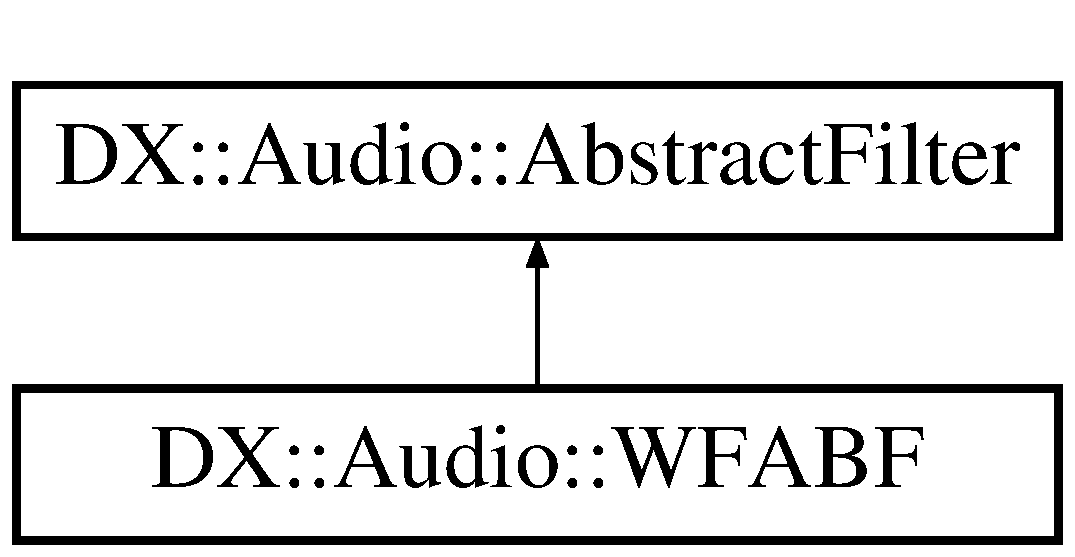
\includegraphics[height=2.000000cm]{struct_d_x_1_1_audio_1_1_w_f_a_b_f}
\end{center}
\end{figure}
\subsection*{Public Member Functions}
\begin{DoxyCompactItemize}
\item 
\hypertarget{struct_d_x_1_1_audio_1_1_w_f_a_b_f_a5a273f168c488f5d5301f26b2672228f}{bool {\bfseries transform\-Packet} (const \hyperlink{class_d_x_1_1_audio_1_1_audio_packet}{Audio\-Packet} \&in, \hyperlink{class_d_x_1_1_audio_1_1_audio_packet}{Audio\-Packet} \&out) const }\label{struct_d_x_1_1_audio_1_1_w_f_a_b_f_a5a273f168c488f5d5301f26b2672228f}

\item 
\hypertarget{struct_d_x_1_1_audio_1_1_w_f_a_b_f_a6af060a5c93a3723cc19659e6ecde5e8}{std\-::string {\bfseries name} () const }\label{struct_d_x_1_1_audio_1_1_w_f_a_b_f_a6af060a5c93a3723cc19659e6ecde5e8}

\end{DoxyCompactItemize}


The documentation for this struct was generated from the following files\-:\begin{DoxyCompactItemize}
\item 
Audio/\-Filters/W\-F\-A\-B\-F.\-h\item 
Audio/\-Filters/W\-F\-A\-B\-F.\-cpp\end{DoxyCompactItemize}

%--- End generated contents ---

% Index
\newpage
\phantomsection
\addcontentsline{toc}{chapter}{Index}
\printindex

\end{document}
